%=======================
% Header
%=======================
\documentclass[11pt]{beamer}





\usepackage{lmodern} 		% Diese beiden packages sorgen für echte 
\usepackage[T1]{fontenc}	% Umlaute.

\usepackage{amssymb, amsmath, color, graphicx, float, setspace, tipa}
\usepackage[utf8]{inputenc} 
\usepackage[english]{babel}
\usepackage[justification=centering]{caption}
\addto\captionsenglish{\renewcommand{\figurename}{}} %Abbildungen nicht bzw. anders beschriften.


%\usepackage[pdfpagelabels,pdfstartview = FitH,bookmarksopen = true,bookmarksnumbered = true,linkcolor = black,plainpages = false,hypertexnames = false,citecolor = black, breaklinks]{hyperref}
%\usepackage{url}
\usepackage{longtable} 		%Seitenübergreifende Tabelle. Vorlage siehe unten
\newtheorem*{bem}{Bemerkung} % Neue Theorem-Umgebung: Bemerkung
\newcommand{\fillframe}{\vskip0pt plus 1filll} 



%-----------------
%BEAMER-SPEZIFISCH
%-----------------

\usetheme{default}
% Verschiedene Varianten von usetheme, usecolortheme und usefonttheme kann man hier ausprobieren: http://deic.uab.es/~iblanes/beamer_gallery/

% \usetheme{
% 	AnnArbor | Antibes | Bergen |
% 	Berkeley | Berlin | Boadilla |
% 	boxes | CambridgeUS | Copenhagen |
% 	Darmstadt | default | Dresden |
% 	Frankfurt | Goettingen |Hannover |
% 	Ilmenau | JuanLesPins | Luebeck |
% 	Madrid | Malmoe | Marburg |
% 	Montpellier | PaloAlto | Pittsburgh |
% 	Rochester | Singapore | Szeged |
% 	Warsaw
% }
%Interessant scheinen: Boadilla, boxes, CambridgeUS, default, (Goettingen), Hannover, Madrid, Montpellier, Pittsburgh, Rochester, Singapore, Szeged, 

\usecolortheme{dove}
% \usecolortheme{
% 	albatross | beaver | beetle |
% 	crane | default | dolphin |
% 	dove | fly | lily | orchid |
% 	rose |seagull | seahorse |
% 	sidebartab | structure |
% 	whale | wolverine
% }

\usefonttheme{structurebold}
% 	default | professionalfonts | serif |
% 	structurebold | structureitalicserif |
% 	structuresmallcapsserif
% }


%\useinnertheme{
% 	circles | default | inmargin |
% 	rectangles | rounded
% } Am besten sein lassen.


% \useoutertheme{
% 	default | infolines | miniframes |
% 	shadow | sidebar | smoothbars |
% 	smoothtree | split | tree
% } Am besten sein lassen.



\setbeamercovered{transparent} %Halbtransparente Overlays (was als nächstes Element auf der Folie gezeigt wird)
\beamertemplatenavigationsymbolsempty % Entfernt Navigationssymbole unten
%\setbeamertemplate{footline}[frame]  % Seitenzahlen
    \setbeamertemplate{footline}{%
    	\raisebox{5pt}{\makebox[\paperwidth]{\hfill\makebox[10pt]{\hyperlink{tableofcontents}{\scriptsize\insertframenumber}}}}}



%---------------------
%--Metainformationen--
%---------------------
\title{Halo and Sub-Halo Finding in Cosmological N-body Simulations}

\author[M. Ivkovic]{
	Mladen Ivkovic
}
\institute[ICS -- UZH]{Institute for Computational Science\\ University of Zurich}

\date[08.12.2017]{08. June 2017}


% \title[Kurzform]{Vortrag zur Berechenbarkeit}
%     Titel des Vortrages
% \subtitle[Kurzform]{Untertitel}
%     Untertitel
% \author[M. Schulz]{Michael Schulz}
%     Autor festlegen
% \institute[IfI -- HU Berlin]{Institut für Informatik\\ Humboldt-Universität zu Berlin}
%     Angabe des Institutes
% \date[26.05.06]{26. Mai 2006}
%     Datum der Präsentation, alternativ kann mittels \date{\today} auch das aktuelle Datum eingetragen werden.
% \logo{\pgfimage[width=2cm,height=2cm]{hulogo}}
%     Die Datei hulogo.pdf (bzw. hulogo.png, hulogo.jpg, hulogo.mps bei Verwendung von pdftex als Backend) als Logo auf allen Folien, hier mithilfe des Paketes pgf.
% \titlegraphic{\includegraphics[width=2cm,height=2cm]{hulogo}}
%     Die Datei hulogo.pdf (bzw. analog wie bei \logo auch entsprechendes Format) als Logo nur auf der Titelseite unter Verwendung des Paketes graphicx.




%-------------------------------
% Neue Befehle
%-------------------------------

\newcommand{\del}{\partial}
%differential d
\newcommand{\de}{\mathrm{d}}

%\newcommand{\ramses}{\textsc{ramses}}
%\newcommand{\phew}{\textsc{phew}}
%\newcommand{\dice}{\textsc{dice}}
\newcommand{\ramses}{\texttt{RAMSES}}
\newcommand{\phew}{\texttt{PHEW}}
\newcommand{\dice}{\texttt{DICE}}

\newcommand{\dt}{\texttt{dice-twobody}}
\newcommand{\ds}{\texttt{dice-levels}}
\newcommand{\cosmo}{\texttt{cosmo}}
\newcommand{\simple}{simple unbinding}
\newcommand{\neigh}{accounting for neighbours}
\newcommand{\iter}{iterative properties determination}
\newcommand{\phewon}{PHEW only}





%===================
% BIBLIOGRAPHY
%===================
\usepackage[backend=bibtex,sorting=nyt,bibencoding=ascii,citestyle=authoryear]{biblatex}
\addbibresource{references.bib}
\usepackage{csquotes} %recommended when using babel and biblatex
%Abbreviations for Bibliography: http://adsabs.harvard.edu/abs_doc/aas_macros.html
\newcommand{\aap}{Astronomy and Astrophysics}
\newcommand{\mnras}{Monthly Notices of the RAS}
\newcommand{\apj}{The Astrophysical Journal}







%=======================
% Document
%=======================
\begin{document}
	
	%--------------------------------------------
	% Stuff that needs to be done before all else
	%--------------------------------------------
	%\pagestyle{plain}
	\nocite{*} % show all entries of bibliography, even if they are not cited.
	
	%-------------
	% Titlepage
	%-------------
	
	%------------------------------------------
%:Metainformationen

\title{\Huge Halo and Sub-Halo Finding in Cosmological N-body Simulations}
%     Titel des Vortrages
%\subtitle{\huge Subtitle}
%     Untertitel
\author{Mladen Ivkovic}
%     Autor festlegen
\affil{Institute for Computational Science \\ University of Zurich \\ Switzerland}
%     Angabe des Institutes
\date{June 2017}
%     Datum der Präsentation, alternativ kann mittels \date{\today} auch das aktuelle Datum eingetragen werden.


%------------------------------------------
	
\maketitle

\begin{center}
	A thesis presented for the degree of\\
	Bachelor of Science in Physics
	
	\vspace{1cm}
	Supervisor: Prof. Dr. Romain Teyssier
	
\end{center}
\vfill
\thispagestyle{empty}
\clearpage

\newpage~\thispagestyle{empty}\newpage
\tableofcontents
\clearpage
	
	%-----------------
	% Actual content
	%-----------------
	\begin{abstract}
	\section*{Abstract}
	\noindent The implementation of a particle unbinding algorithm into the adaptive mesh refinement (AMR) code \ramses, which uses the segmentation algorithm \phew\ to identify halos and their substructure in simulations of collisionless dark matter is presented.
	Only particles initially assigned to subhalos are examined, particles of halos are assumed to be bound.
	The algorithm follows the hierarchy of substructures as found by \phew\ and passes unbound particles on to the next higher level of substructure for examination.
	Furthermore, it accounts for neighbouring structures by demanding a particle to be exclusively bound to the subhalo that is being investigated.
	In order to increase the accuracy of the substructure's properties, they are determined iteratively by taking into account only bound particles.\\
	%
	The algorithm is fully parallel and uses the MPI library.
	Its effects, accuracy and resource usage are shown on two highly idealistic datasets and a cosmological simulation.
\end{abstract}
	

\begin{frame}
	\frametitle{Cosmological N-body Simulations}
	
	\begin{itemize}
		\item N-body simulations are simulations of the motion of particles under the influence of physical forces.
		\item Focus on collisionless dark matter particles: 
		
		\begin{itemize}
			\item   hypothetical type of matter 
			\item 	the only significant interaction between the particles is via gravity
		\end{itemize}
	
	\end{itemize}
	
\end{frame}








\begin{frame}
	\frametitle{Cosmological N-body Simulations}
	
	\begin{itemize}
		\item After some time, the particles will clump together. Such gravitationally bound objects are called \emph{halos}.
		\item Halos themselves may contain self-bound objects, called \emph{subhalos}.
		\item The identification of halos and subhalos is an important tool for problems concerning cosmic structure and its formation.
		\item Codes that perform this task are called \emph{halo-finders}.
	\end{itemize}
	
\end{frame}














\begin{frame}
	\frametitle{Cosmological N-body Simulations}

	\begin{columns}
		\column{.25\textwidth}
			The results of a cosmological simulation of $128^3$ dark
			matter particles at redshift $z = 0$ with $H_0 = 70.4$ and density parameters $\Omega_m = 0.272$ and $\Omega_\Lambda= 0.728$.
			The box length corresponds to 88.8 Mpc.
			\vfill
		\column{.75\textwidth}
			\begin{figure}
				\centering
				\includegraphics[width=8.2cm]{../report/images/cosmo/cos-part2map-npart.png}
		%		\caption{
		%		}
			\end{figure}
		\vfill
	\end{columns}

\end{frame}










\begin{frame}
	\frametitle{Unbinding Particles}


	\begin{itemize}
		\item By convention, it is customary to treat all particles assigned to a halo as bound to it, even though from a strict energetic perspective they may not be.
		\item For subhalos, on the other hand, it is vital to identify and remove unbound particles:
		\begin{itemize}
			\item Subhalos are located within a host halo and therefore expected to be contaminated by the host's particles
			\item Usually subhalos contain far less particles than their hosts, so assigning particles to it without an unbinding procedure can influence its physical properties significantly.
		\end{itemize}
		\item ``Removing a particle'' means here to assign it to the parent structure. This applies recursively to any level of substructure within substructure.
	\end{itemize}


\end{frame}







\begin{frame}
	\frametitle{Goals of this thesis}


	\begin{itemize}
		\item \ramses\ \parencite{ramses} is a N-body and hydrodynamical code that %
		contains a clump finding algorithm, \phew\ \parencite{PHEW}.
		%makes use of the adaptive mesh refinement technique: The entire computational domain is covered by cells, and smaller and smaller cells are introduced where necessary to achieve the desired accuracy.
%		\item \phew\ \parencite{PHEW} is a clump finding algorithm that can identify halos on-the-fly within the framework of \ramses.
		
		\item Both \phew\ and \ramses\ are fully parallel and make use of the MPI library. \phew\ works on-the-fly.
		
		\item The goal of this thesis is to implement a particle unbinding algorithm to work with \phew\ that is also fully parallel and works on-the-fly.
	\end{itemize}



\end{frame}









	\section{Theory}








\subsection{Overlying Framework: {\normalfont \scshape RAMSES} and {\normalfont \scshape PHEW}}



%==============================
% RAMSES
%==============================



\subsubsection{{\normalfont \scshape RAMSES}}

\ramses\ is a N-body and hydrodynamical adaptive mesh refinement (AMR) code which uses the ``Fully Threaded Tree'' data structure of Khokhlov \parencite{FTT}. 
It simulates the time evolution of particles.
The domain is covered by a Cartesian grid, called the mesh.
Simulations require numerical integration, whose accuracy increases as the size of a grid cell decreases, but smaller grid cells naturally need more resources to cover a domain of the same size.
AMR is a method that ``\textit{tries to attain a fixed accuracy for a minimum cost}'' \parencite{AMR} by ``refining'' the mesh only where and when necessary.
``Refining'' in this case means that cells of smaller and smaller sizes are introduced until the desired accuracy is achieved.
Grid cells that contain lots of particles will be refined many times, while grid cells that contain no particles won't be refined at all.
The unrefined grid is called the ``\emph{coarse grid}'' and the number of times a cell of the coarse grid is refined is called the ``level of refinement''.
Cells which are not refined (any further) are called ``\emph{leaf cells}''.
They always have the highest level of refinement at their position.

The basic elements of the data structure in \ramses\ are groups of $2^{\text{dim}}$ sibling cells called ``\emph{octs}''.
Each oct belongs to a given level of refinement. 
All octs of a given refinement level are sorted in a doubly linked list, so each oct points to the previous and the next oct in the linked list of the particular level.
The fully threaded tree structure also demands that each oct points to the parent cell (the cell on the less refined level) as well as the $2 \cdot \text{dim}$ neighbouring parent cells and the $2^{\text{dim}}$ child octs on the next refinement level, assuming they exist. \\
%The cells on the least refined level are called the coarse grid. 
%To dynamically modify the AMR structure at each time step, first all cells are being marked for refinement according to user-defined criteria. 
%Any oct in the tree structure must be surrounded by $3^{\text{dim}}-1$ neighbouring parent cells, which enforces a smooth transition in spatial resolution.
Particles belonging to octs are organised in linked lists as well. 
A particle belongs to a particular oct if its position fits exactly into the oct boundaries, and all particles that belong to the same oct are linked together by a linked list. 
%Each oct can access the first particle of its linked list and the number of particles its list contains.

A system that contains many particles is called a ``N-body system''.
A collisionless N-body system is described by the following equations for the particles with position $\vec{x}_p$ and velocity $\vec{v}_p$:
	\begin{align}
		&\frac{\de\vec{x}_p}{\de t} =  \vec{v}_p &\frac{\de\vec{v}_p}{\de t} = - \nabla_x \phi 
	\end{align}
%
with
%
	\begin{align}
		 &\Delta_x \phi = 4 \pi G \rho \label{eq:poisson}
	\end{align}	
%
Where $\phi$ is the potential, $G$ the gravitational constant and $\rho$ the mass density field.
To compute the spatial movement of the particles, first $\rho$ is computed using a ``\emph{Cloud-In-Cell}'' (CIC) interpolation scheme.
The CIC scheme considers all particles to be cubes (``clouds'') of one cell size and of uniform density. 
The mass of a particle is deposited in cells based on what fraction of its ``cloud'' overlaps with the cell, thus determining the density field.
Once the density field is known, the Poisson equation (\ref{eq:poisson}) can be solved numerically and the potential $\phi$ is computed. 
Now the acceleration for each cell can be obtained, from which the particle acceleration $\tfrac {\de\vec{v}_p}{\de t}$ is computed using the inverse CIC interpolation. 
The acceleration is then integrated over time to compute the particle velocity $\vec{v}_p$ and position $\vec{x}_p$ using a second-order midpoint scheme.

%For a more detailed description of the code, I refer the reader to the release paper of \ramses\ \parencite{ramses}.

















%==============================
% PHEW
%==============================




\subsubsection{{\normalfont \scshape PHEW}} \label{chap:phew}

\phew\ is a structure finding algorithm implemented into \ramses. 
It is a ``watershed-based'' algorithm: ``\textit{These algorithms assign particles or cells to density peaks by following the steepest gradient, resulting in the so called `watershed segmentation' [...] of the negative density field.}'' \parencite{PHEW}.
%In the case of \ramses, \phew\ is applied to the mass density field defined by the projection of the particles' mass on the mesh.
\phew\ groups cells together by separating the mass density field along minima, thus dividing the density field into patches.
The density field is obtained with the deposition of the particle's mass on the mesh through CIC interpolation.
The algorithm can be divided in four main steps: segmentation, connectivity establishment, noise removal and substructure merging. 

In the first step, namely the ``watershed'' segmentation, the cells of interest are identified. % and their neighbours stored. 
%on the mesh are grouped together into patches around a local density maximum called the peak. 
These are all leaf cells which have a density above an user-defined density threshold and are called ``\emph{test cells}''.
If a cell doesn't have a denser neighbour, it is marked as a local density peak and assigned a peak label.
The peak label of a cell defines what peak patch this particular cell belongs to.\\
Then each cell copies the peak label from its densest neighbour.
This way, each cell is assigned to the peak ``closest'' to it by following the path of rising density. 
All test cells assigned to a particular peak form the aforementioned peak patch.
The separating surface between peak patches will be cell borders which contain local density minima, corresponding to the watershed analogy.

%In order to perform this segmentation, all leaf cells which have a density above an user-defined density threshold are marked. 
%These cells are called "test cells". 
%The neighbour cell with the highest density of each test cell is stored. 


%The test cells are then sorted by decreasing density and each cell copies the peak label from its most dense neighbour.
%Because the cells have previously been sorted, their densest neighbour will always have a peak label: Either it was a peak to begin with, or it has been accessed before because it is more dense.


In the next step, the connections between the peak patches need to be established. 
All test cells are examined for neighbours that belong to another peak. 
If a neighbouring cell with a different peak label is found, the density of the common surface between those two neighbours is defined as the average of these two cell densities.
%Obviously the connecting surface between two peak patches can consist of (surfaces of) multiple cells. 
The maximal surface density between two particular peak patches is considered as the ``\emph{saddle}'' between these two. 
Naturally, a peak patch can have multiple neighbouring peak patches. 
Out of all the saddles of all the neighbouring peak patches, the one with the highest density is called the ``\emph{key saddle}'' and the neighbour it connects to is referred to as the ``\emph{key neighbour}''.

The third main step, noise removal, requires a clear definition of what is to be considered noise. 
In \phew, each peak patch is assigned a value representing the contrast to the background called ``\emph{relevance}''.
A peak patch's relevance is defined as the ratio of the peak's density to its key saddle. 
A peak patch is considered noise if the its relevance is lower than a user-defined relevance threshold.
An irrelevant peak patch is then merged to its key neighbour. 
If an irrelevant peak patch doesn't have a key neighbour because it is isolated, it is discarded.



Expressed explicitly, merging a peak patch $i$ into a peak $j$ means that all cells of $i$ inherit the peak label of $j$.
%Due to these conditions, just like the test cells in the watershed segmentation step, the peaks are sorted by decreasing peak density in order to enable the propagating peak labels to travel as far as possible in one loop.
%In order to perform the noise removal, like in the segmentation step with the test cells, all peaks are sorted by decreasing density.
%This sorting makes sure that the noise removal can be executed in one loop only. 
Both peaks' saddles are merged as well: 
The peak patch $j$ inherits the saddles that connected $i$ to other patches.
Therefore, after two peaks are merged, new key saddles and the relevance need to be determined for the peak patches that have undergone merging.
%introduce loop here fso you don't have to later
%To maximise performance, the merging step is executed in a loop on peak patches sorted by decreasing density. 
This concludes the noise removal, since all irrelevant patches are either merged into relevant peaks or discarded.\\
%
%The last main step of the algorithm is merging of the peak patches.
As mentioned before, \phew\ can work in parallel on multiple processors.
The parallel implementation will be discussed in more detail in section \ref{chap:parallel}.
In order to produce unique results when executed on multiple processors, the merging of peak patches needs to obey the following three rules:
%
\begin{enumerate}
	\item Whether a peak should be merged into its key neighbour or not is determined by some criterion.
	\item A peak patch is only merged into its key neighbour.
	\item The peak of the key neighbour must have a higher density.
\end{enumerate}
%
In the case of noise removal, the criterion is to satisfy the relevance condition. The criterion is different for the substructure merging step.\\
%
Once the noise removal step is completed, the remaining structure consists only of peak patches which satisfy the relevance condition and is referred to as ``\emph{level 0 clumps}''. 
These clumps represent the structure on the lowest scale.
A large halo for example, which can very roughly be described as ``a large clump'' in a first approximation, would be decomposed into many small clumps. In order to identify such a halo as a single object, one more step is necessary.


The identified level 0 clumps can be merged further into composite clumps.
The procedure used is exactly the same as in the previous step, only the merging criterion is different:
The new criterion is a threshold for the key saddle density. All peak patches whose key saddle density is \emph{higher} than the user-defined threshold are merged into their key neighbour.
The saddle threshold defines which clumps should be considered as separate structures and which should be  merged and considered as composite structures.\\
%
After the first round of merging, the lowest level of structure has been merged into first composite clumps.
If clump $a$ is merged into clump $b$, then $b$ is called the ``\emph{parent}'' of $a$.
Because of the merging, again the lists of saddle points change for the ``surviving'' clumps, and the list as well as the key saddles need to be updated.
The peak labels of the cells however are not updated in this merging procedure: 
They are necessary to preserve the information on substructure.
Only the clump properties like volume, mass, position and neighbours are merged.\\
%
The merging of clumps creates connections between peak patches where there were none before in the sense that the surviving peak patches can establish a connection to other surviving patches because clumps between them were merged into them.
See for example in figure \ref{fig:phewlevels}: The red and the blue clump establish a connection after all the smaller clumps between them have been merged into them in the span of two merging loops.
Each merging loop then represents a different level of substructure:
In each loop, greater structures are being merged into each other than there were in the loop before.
Starting from the lowest level, which are the peak patches identified after noise removal, clumps are merged into each other until none satisfy the merging criterion any more.
%Figure \ref{fig:phewlevels} illustrates the concept of the described merging hierarchy.
%

\begin{figure}[htbp]
%\parpic[r]{%
\centering
	\fbox{
		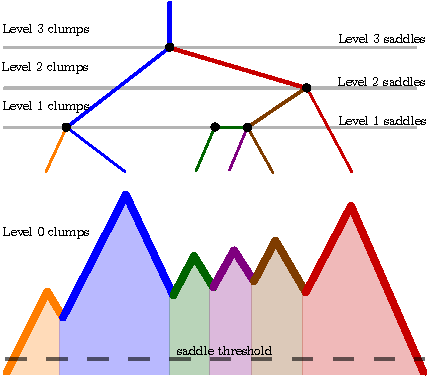
\includegraphics[width = 9.5cm, keepaspectratio]{images/phew/saddle_hierarchy2.pdf}
	}
	\caption{
		Hierarchy of clumps as created by \phew's clump merging algorithm. 
		Level $n$ saddle points are used for merging during the $n-$th round of merging. 
		A peak patch is always merged into its key neighbour and it is only merged into a peak patch with a higher density.
		In this figure, the merging criterion is that the key saddle is higher than the saddle threshold.\\
		Image adapted from \cite{PHEW}}
	\label{fig:phewlevels}
\end{figure}
%

When the merging is finished, the clumps have been merged into the largest possible structures that satisfy the relevance and saddle density conditions.
The remaining structures are large clumps and they are considered as halos, provided that the clumps are massive enough.
A halo must have a minimal mass that can be set by the user.\\
%
The label of halos will be the label of clumps which are never merged into an other, but only have other clumps merged into them. 
Such clumps are called ``\emph{halo-namegivers}''.



In summary, \phew\ identifies halos by the following three criteria:
\begin{itemize}
	\item {Halos are composed of cells with densities above a density threshold.}
	\item{A halo must have a minimal mass that can be set by the user.}
	\item {Within a halo, the subhalos are peak patches that are relevant, i.e. aren't considered noise. Their edge is determined by local density minima surfaces.}
	\item {If the interface between two relevant peak patches is less dense than a threshold (saddle threshold), the two peak patches are considered to be two independent halos.}
\end{itemize}




%Since \ramses\ is a parallel code which uses the MPI library and the fundamental strategy of splitting the computational domain between MPI tasks, \phew\ must be able to work in parallel on the split domain as well.
%This is not a trivial task since the watershed segmentation is non-local by nature.
%This concludes the description of the way \phew\ works. 
%I will describe the parallel implementation of \phew\ (and \ramses) briefly and simplified in the following section, while focussing on the parts and tools necessary for the unbinding code. 
%For a more detailed description of \phew\, I refer the interested reader to its release paper \parencite{PHEW}.

%Splitting the computational domain between multiple MPI tasks is realised by introducing virtual boundaries.
%Instead of having data of the whole computational domain, each MPI task has only the knowledge of its own part of the domain.
%Around the computational domain of each MPI task, there is a so called "virtual domain". 
%All necessary data from other MPI tasks is communicated with MPI tools into the so called virtual domain, which surrounds the "real domain", so that the virtual domain mimics what happens in the domains of other tasks.
%This way, only the necessary information needs to be transferred and the code can be executed on distributed memory computers.




%\ramses\ advances the timely evolution of the particles timestep by timestep, thus creating a snapshot of the particles' position and velocity at each timestep. 
%\phew\ can then be executed on the results of the time advancement, meaning that the segmentation is only performed on snapshots of the simulation. 
%This yields the segmentation of the density field into patches at every timestep (that is on every required timestep that would be stored as output), but the patches found can't be tracked trough time:
%Only one more or one fewer local density maximum would shift all peak indices by which the peaks are labelled. 
%
%The peak patches correspond in the case of particles to spatially separated regions with a density higher than a given density threshold.
%Such regions are commonly referred to as \emph{clumps} of particles and \phew\ is also called a \emph{clumpfinder}.
%


















\subsubsection{Parallel implementation}\label{chap:parallel}

\ramses\ is a parallel code which makes use of the MPI library.
The use of MPI (message passing interface) allows a process on a distributed memory architecture to be executed in parallel by multiple tasks and enables various types of communications between them.
 
The fundamental parallelisation strategy used in \ramses\ is domain decomposition,
where a part of the total spatial computational domain is assigned to each processing unit, or ``MPI task''.
It makes use of the fact that most calculations on grids do not require the knowledge of the entire computational domain, but only the cells in their vicinity
The basic idea of the domain decomposition is illustrated in figure \ref{fig:parallel}, where a 2D-grid is split between two processors. 
The partial domains do not overlap and a thin layer of cells called the ``\emph{virtual boundary}'' is introduced where the domain was cut. 
Necessary information is then communicated across MPI tasks from the other tasks' ``real domain'' into the virtual boundary, so that the virtual boundary copies what happens in the domains of other tasks and allowing the execution of the code as if the domain wasn't split.
Two tasks working on the same problem allows a much faster execution time, but it also enables the solution of a much bigger problem that only one task couldn't do on its own, e.g. because of memory restrictions.

\begin{figure}[htbp]
	%\parpic[r]{%
	\centering
	\fbox{
		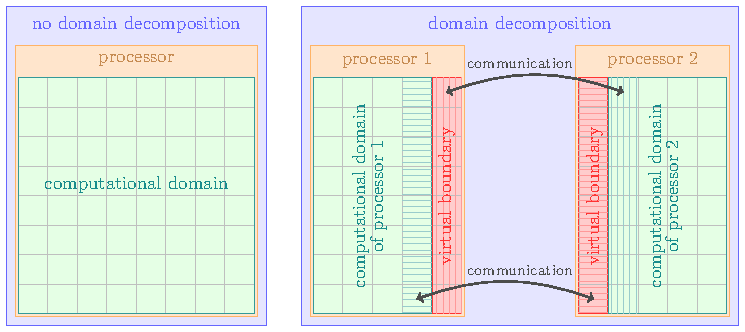
\includegraphics[width = 12.5cm, keepaspectratio]{images/tikz/parallelisation.pdf}
	}
	\caption{
		The basic idea of domain decomposition. Here a 2D-grid is split between two processors (right) instead of only one (left). 
		The partial domains do not overlap and where the domain was cut, a  ``virtual boundary'' is introduced. 
		Necessary information is then communicated between processors from the other tasks' ``real domain'' into the virtual boundary, so that the virtual boundary copies what happens in the domains of other tasks and allows the execution of the code as if the domain wasn't split.
	}
	\label{fig:parallel}
\end{figure}




\phew\ uses the virtual mesh boundary as well, since every cell on each domain must have the information of all its neighbours.
%by shifting the local peak index to an interval of indices reserved only for one particular task.
%The reserved interval is determined by the number of peaks found by all tasks.
%Every task has an interval of peak indices reserved for itself, making the global peak index unique.
%During the segmentation loop, all cells that change their peak patch label are counted. 
%The segmentation step, which is executed in a loop, is repeated until there are no more changes of peak labels of cells on the entire computational domain.
%The peak patch labels in the virtual boundary
%are updated using MPI communications before every loop.\\
%
Initially, all peaks are counted and their number is communicated throughout all MPI tasks.
This gives all MPI tasks the knowledge of the total number of peaks of the entire computational domain, allowing the introduction of a peak label that is globally unique for each peak. 

Similarly to the virtual mesh boundary, a virtual peak boundary is necessary.
For the peak patch merging step, each peak patch on each task's domain needs the information of the peak patches that surround it.
If, for example, a peak patch is split in two by the domain boundaries between two tasks, both tasks need to know all the peak patch's neighbours on the other task's domain.\\
%
Unlike the mesh boundary however, the virtual peak boundary is not a fixed region in space.
Because of the merging, peaks gain neighbours they hadn't had before.
This requires that new peaks are introduced to the virtual peak boundary during the merging procedure.
%Virtual peaks are introduced by assigning them a local peak index.
%Each tasks stores the virtual peaks in the first free place in the memory after the ``real'' peaks.
Once introduced, all other peak properties, e.g. its relevance and saddle points, can be transferred by means of MPI communication.

The virtual peak boundary requires two types of communications. 
One type is the collection (sum, minimum or maximum) of a value for a peak from all tasks which have that particular peak patch in their virtual boundary to the owner of the peak.
The ``\emph{owner}'' of the peak is the task where the density peak is in the ``real'' domain, as opposed to the virtual mesh boundary.
Imagine for example the calculation of a peak patch's total volume on multiple tasks: 
Each task would compute the volume of that peak patch on its own domain and then all these partial results would be sent to the peak's owner and summed up.\\
%
In that scenario only the peak's owner has the total volume of the patch, but the ones that have it in their virtual boundary still only have their partial values.
This brings us to the second required type of communication:
A scatter of data from the owner of the peak to all tasks with that particular peak in their virtual boundary. 
In our example, the owner of the peak would send the computed total volume of the peak patch to all the tasks which require that information. 
%In this case, the value of the boundary peaks is overwritten by the new data.\\
%
In order to perform these communications, a communication structure (called the ``peak communicator'') must be built first. 
The purpose of the peak communicator is to establish how many peaks of every task are owned by any other task, or in other words: ``what needs to be sent (and received from) where''.
Once that is known, the communications between the processes and thus the parallel merging can be performed.



The following summary of results and tools available after the execution of the segmentation algorithm concludes this brief description of \phew\ and \ramses:
%
\begin{itemize}
	\item A list of peak patches, composed of overdense leaf cells, representing clumps of particles
	\item A hierarchy of these clumps, established during the merging of the peak patches
	\item A virtual boundary for cells and another virtual boundary for peak patches along with as a set of communication tools which enable the transfer of peak patch information across MPI tasks.
\end{itemize}



%Now that the N-body and the segmentation algorithms are introduced, I would like to discuss in the next section what `unbound' particles are.























%======================
%Unbinding
%======================





\subsection{Unbinding Particles}



\subsubsection{Constraints and Limitations}

%In this section I will discuss what conditions need to be satisfied in order for a particle of mass $m_p$ and velocity $\vec{v}_p$ to be considered as "bound".




%I will discuss the physical meaning of eq. \eqref{eq:bound} later.
%First I need to establish what assumptions I make and how I describe the system of particles in order to gain an expression for the energy $E$ which can be interpreted and calculated.



Due to complexity and size, solutions of physical problems often require simplifications and assumptions to be made.
In this section, the assumptions necessary for the unbinding algorithm are explained shortly.

Firstly, the situation under consideration is assumed to be \emph{time-independent}.
This allows an easy description of the system by introducing local energy conservation on one hand, but on the other hand, the information necessary for a time-dependent description is not readily obtainable.
\ramses\ computes the evolution of the particles time step by time step, thus creating a snapshot of the particles' position and velocity at each time step. 
%The particles represent collisionless dark matter particles.
\phew\ can then be executed on the results of the time advancement, meaning that the segmentation is only performed on snapshots of the simulation. 
%This yields the segmentation of the density field into patches at every time step (or rather on every required time step that would be stored as output).
In order to obtain the information necessary for a time-dependent description, the entire simulation from beginning to end must be known, which contradicts the requirement for on-the-fly analysis.
Furthermore, due to the nature of \phew, the found peak patches can't be tracked trough time:
Only one more or one fewer local density maximum would shift all following peak labels.
%This leads to the first restriction: I must consider the system to be \emph{time independent}. 


The purpose of a particle unbinding algorithm is to determine for each particle of a (sub)structure if the particle is bound to that particular structure. 
%, which means to determine if it satisfies the condition (\eqref{eq:bound}) or not.  
The focus on the substructure itself, as opposed to a global perspective, leads to the second used simplification: 
The structure is considered to be \emph{isolated}.
Any effects on the particles that arise from outside the structure that is being investigated, e.g. tidal effects, are neglected.
(Some consequences of neighbouring structures will be accounted for, which is will be discussed in section \ref{chap:neighbours}).
This simplification is also motivated by the enormous computational expense that would arise from taking the entirety of structures in the computational domain into account for each substructure anew.

Lastly, a third major simplification is used.
As will be introduced more properly in the following section, whether particles are bound to a clump depends on the gravitational potential of the clump itself.
In classical mechanics, the gravitational potential $\phi(\vec{r})$ is determined by the poisson equation \ref{eq:poisson}.
%%
%\begin{align}
%	\Delta \phi(\vec{r}) = 4 \pi G \rho(\vec{r}) \label{eq:poisson}
%\end{align}
%%
%where $\Delta$ is the Laplace operator, $G$ is the gravitational constant and $\rho$ is the mass density field. 
It represents the amount of work needed to move the particle from infinity (where as a point of reference the potential is usually chosen to vanish) to the place it is.\\
%
In theory, equation \ref{eq:poisson} can be solved, because if all the particle positions are known, then the density field $\rho$ is known as well.
Sadly the solution for each particle depends on each other particle, so calculating it makes it a computationally expensive code of order $\mathcal{O}(N^2)$.
This is not acceptable for a code required to work on-the-fly.
Instead, an analytical solution which is valid for \emph{spherically symmetric} systems is used.
%Consider a spherically symmetric clump of radius $r_{max}$ such that there are no more particles further away from the centre of mass than $r_{max}$ and total mass $M_{tot}$.
It is a bit unfortunate to introduce the assumption of spherical symmetry, because \phew\ had no need for it and was able to identify clumps of any shape, an information which is ignored at this point.
Nonetheless, due to the lack of a better solution at this time, it was a necessity.





To summarise, each substructure clump as found by \phew\ is considered to be an isolated, time independent spherical system of collisionless dark matter particles.



















\subsubsection{Bound Particles}

In general, one can assign every particle a total energy $E$. 
A particle is considered to be ``\emph{bound}'' if
%
\begin{align}
	E < 0 \label{eq:bound}
\end{align}
%
or ``\emph{unbound}'' if it doesn't satisfy this condition.
%In order to determine an expression for the total energy $E$ of a particle, one must first establish the manner in which the system of particles will be described, particularly which assumptions are made.
%The assumptions, on the other hand, are influenced by the system to be described, but also by the result one is trying to achieve.
%So we need to have a look at ``what we have'' and ``what we want''.

Consider now an isolated clump that is made up of $N$ particles, where the position $\vec{x}_i$, the velocity $\vec{u}_i$ and the mass $m_i$ of every particle $i$ is known. 
Even though the system is assumed to be time independent, the structures within the system do not need to be stationary.
On the contrary: The clumps are expected to be in motion with respect to the computational grid.
It is often useful to consider the problem in another frame of reference, namely the ``centre of mass'' frame.
The centre of mass of a clump of $N$ particles is defined as:
%
\begin{align}
	\vec{x}_{CoM} = \frac{\sum_{i=1}^{N} m_i \cdot \vec{x}_i}{\sum_{i=1}^{N} m_i} \label{eq:com}
\end{align}
%
%Where $N$ is the number of particles of the clump. 
The centre of mass frame is then defined as the frame of reference where the velocity of the centre of mass (also called the ``\emph{bulk velocity}'') vanishes:
%
\begin{align}
	\vec{v}_{CoM} = \frac{\de}{\de t} \vec{x}_{CoM}  = \frac{\sum_{i=1}^{N} m_i \cdot \vec{u}_i}{\sum_{i=1}^{N} m_i} \equiv 0 \text{ \hspace{5mm} in centre of mass frame} \label{eq:vcom}
\end{align}
%
and the centre of mass is at the origin:
%
\begin{align}
	\vec{x}_{CoM} \equiv 0
\end{align}
%
The particle positions and velocities in the centre of mass frame are then
%
\begin{align}
	\vec{x_i}\ ' &= \vec{x_i} -\vec{x}_{CoM} \equiv r_i\\
	\vec{u}_{i}\ ' & = \vec{u}_i - \vec{v}_{CoM} \equiv \vec{v}_i \text{\hspace{1cm} with \hspace{1cm} }  v_i \equiv ||\vec{v}_i|| = \sqrt{v_{x,i}^2 + v_{y,i}^2 + v_{z,i}^2}
\end{align}
%

The assumption of time-independence and isolation allow to describe the clump by means of classical mechanics.
In such a system the energy $E_i$ of a particle $i$ in the centre of mass frame of the clump it belongs to can be expressed as 
\begin{align}
	E_i = T_i + V_i = \frac{1}{2} m_i \cdot v^2_i + m_i \phi (\vec{r}_i)\label{eq:E}
\end{align}
%
and is conserved:
\begin{align}
	E_i = const
\end{align}
Where $T_i = \tfrac{1}{2}m_p v_i^2$ is the \emph{kinetic energy} and $V_i = m_i \cdot \phi(\vec{r}_i)$ is called the \emph{potential energy} of the particle. 
$\phi(\vec{r}_i)$ is called the \emph{potential}.
%The expression for $\phi$ is discussed in the next section.
%In scope of this section, it suffices to note that $\phi \leq 0$ .

Plugging equation \eqref{eq:E} into the condition for a particle to be bound \eqref{eq:bound}, we get
%
\begin{align}
	\frac{1}{2} m_i \cdot v_i^2 + m_i \phi(\vec{r}_i) < 0
\end{align}
%
Or equivalently:
%
\begin{align}
	v_i < \sqrt{- 2 \cdot \phi(\vec{r}_i)} \label{eq:boundv}
\end{align}
%
These equations allow for an evident physical interpretation of the criterion for a particle to be bound:
It is bound if its kinetic energy is lower than the absolute value of the (gravitational) potential that it experiences. 
A bound particle's movement will be constrained by the potential:
The potential will always pull the particle towards the centre of mass of the clump. 
It can not escape arbitrarily, but will orbit the clump on elliptic trajectories.
%Equation \eqref{eq:boundv} also leads to the definition of the escape velocity $v_{esc}$:
%
%\begin{align}
%	v_{esc} = \sqrt{-2 \phi} \label{vesc}
%\end{align}
%
%Which is the minimal velocity a particle needs to have for it not to be bound to the clump.
%Equivalently to equation \eqref{eq:boundv}, a particle is considered bound if:
%\begin{align}
%	v < v_{esc}
%\end{align}
%%
%Or to put it in simple words: A particle is considered bound if it cannot escape the spatial boundaries of the potential that it experiences. 


$\vec{r}_i$ and $\vec{v}_i$ are known for each particle.
What remains to be found is an expression for the potential $\phi$.
Since only isolated collisionless dark matter particles are considered, the potential that influences the particles is the gravitational potential of the particles themselves.
In a spherically symmetric system, the potential at each point is determined by the absolute (radial) distance as opposed to its exact location.
Thus the potential can be expressed in the clump's centre of mass frame as $\phi(\vec{r}_i) = \phi(d_i)$ with 
\begin{align}
	d_i = \sqrt{(r_{i,x}-x_{CoM,x})^2 + (r_{i,y}-x_{CoM,y})^2 + (r_{i,z}-x_{CoM,z})^2}
\end{align}

The spherically symmetric Poisson equation (eq. \ref{eq:poisson}) can be solved for $\phi$:
%
\begin{align}
	\phi (r_i) &=  - G \int\limits_{r_i}^{r_{max}} \frac{M(<\tilde{r})}{\tilde{r}^2} \mathrm{d}\tilde{r}
	- G  \frac{M_{tot}}{r_{max}}
	\label{eq:sol_phi}
\end{align}
%
Where $M(<r) \equiv \int\limits_0^r 4 \pi \rho(\tilde{r})\tilde{r}^2 \mathrm{d}\tilde{r} $ is the mass enclosed by a sphere of radius $r$ such that the clump's total mass is enclosed by the radius $r_{max}$: $M_{tot} = M(<r_{max})$.
The full derivation of equation \eqref{eq:sol_phi} is given in appendix \ref{app:sol_phi}.


%The general idea is to simplify the poisson equation (eq. \eqref{poisson}) by assuming spherical symmetry of the problem and then solving the equation with an assumed density function $\rho (r)$.



















\subsubsection{Accounting for Neighbouring Structures}\label{chap:neighbours}

The boundaries of a particle's trajectory in a given potential $\phi$ can be estimated using the conservation of energy:
%
\begin{align}
	E/m_p = \frac{1}{2} v^2 + \phi = const.
\end{align}
%
A gravitational potential is qualitatively shown in figure \eqref{fig:orbits} as well as a particle $\alpha$ with $\frac{1}{2}v^2 < - \phi$.
The total energy per particle mass $E/m_p$ of the particle on the graph is then exactly the difference between the negative potential and the kinetic energy on the $y$-axis.
In order to conserve energy, the curve of possible kinetic energies (dotted line in figure \ref{fig:orbits}) that the particle may take on will always have the same distance $E/m_p$ from the negative potential curve.
Because $v^2\geq 0$, the spatial boundaries of a particle's trajectory can be found by following the curve of possible kinetic energies of the particle to the point where $v^2 = 0$.

\begin{figure}[h!]
	\centering
	\minipage[t]{0.45\textwidth}
	%\centering
	\fbox{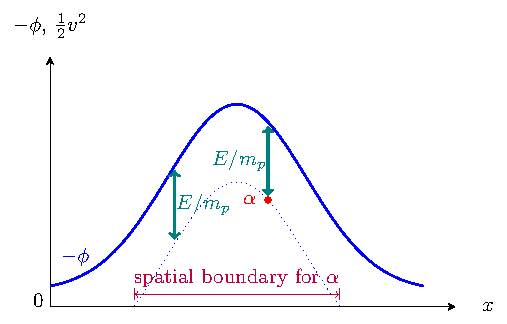
\includegraphics[height=4.45cm, keepaspectratio]{images/tikz/boundaries.pdf}}%
	\caption{A qualitative plot of a potential $\ -\phi$ and a particle $\alpha$. 
		The boundaries of the particle's trajectory can be found using energy conservation $E/m_p = \frac{1}{2}v^2 + \phi$ by following the curve of the particle's kinetic energies (dotted line) to the points where $v^2=0$.	
	}%
	\label{fig:orbits}
	\endminipage%\hspace{.1cm}
	\hspace*{\fill}
	%
	\minipage[t]{0.55\textwidth}
	%\centering
	\fbox{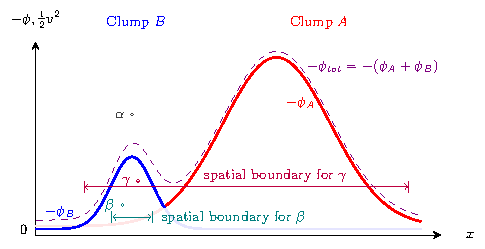
\includegraphics[height=4.45cm, keepaspectratio]{images/tikz/potentials.pdf}}%
	\caption{Qualitative potential of a halo containing two clumps $A$ and $B$. Three particles assigned to $B$ are shown: $\alpha$ is not bound to $B$, $\beta$ is bound, $\gamma$ satisfies the energy condition to be bound, but can wander off into clump $A$ and shouldn't be considered as such.
	}%
	\label{fig:potentials}
	\endminipage\hspace*{\fill} 
\end{figure}
%
This fact changes the situation significantly for the interpretation of what particles should be considered bound as follows.
Consider now an isolated halo that consists of two clumps, $A$ and $B$, where $B$ is a smaller clump nested within clump $A$.
Their potentials are qualitatively depicted in figure \eqref{fig:potentials}. 
Three particles assigned to $B$ with different kinetic energies are marked, representing three different cases:
%
\begin{itemize}
	\item Particle $\alpha$ has a kinetic energy higher than the potential, it is clearly not bound to the clump $B$.
	\item Particle $\beta$ has a kinetic energy lower than the potential at that distance from the centre of mass, so it will remain bound on an elliptic trajectory around the centre of mass.
	\item Particle $\gamma$ is considered energetically bound to the clump just like $\beta$, i.e. it satisfies the condition \eqref{eq:boundv}, but it won't necessarily remain on an elliptic trajectory around clump $B$'s centre of mass: Because of clump $A$'s neighbouring potential, the particle can leave the boundaries of clump $B$ and wander off deep into clump $A$.
\end{itemize}
%

These considerations show that due to the fact that subhalos will always have neighbouring structure, there will be particles like $\gamma$ that can wander off into neighbouring clumps even though they satisfy condition \eqref{eq:boundv}.
It is obvious that particles like $\gamma$ shouldn't be considered as bound and that therefore the bound condition needs to be modified appropriately.
Even though the clumps were assumed to be isolated, clumps that make up substructure will always have at least one neighbour by their nature.
The reason $\gamma$ can wander off is because its boundary extends past the interface that connects the two clumps, so the condition for a particle to be bound must be that its trajectory must never reach that interface.
Defining $\phi_S$ to be the potential of clump $B$ at the interface to the neighbouring structure that is closest to $B$'s centre of mass, the condition for a particle to be bound \emph{exclusively} to a particular clump can be written as
%
% Need energy to be ``more negative'' !
\begin{align}
	E/m_p = \frac{1}{2}v^2 + \phi -  \phi_S < 0
\end{align}
%
or equivalently:
%
\begin{align}
	v < \sqrt{ - 2(\phi - \phi_S) } \label{eq:boundv_corr}
\end{align}


According to the argumentation above and figures \ref{fig:orbits} and \ref{fig:potentials}, it is to be expected that demanding particles to be exclusively bound will find more unbound particles than not doing so, where particles close to the centre of mass should be more likely to be exclusively bound than the particles closer to the edge of the subhalo.












\subsubsection{Structure Hierarchy: What to Do With Unbound Particles}

One last thing that needs to be considered with respect to unbinding particles is the hierarchy of substructures that is found by \phew, as described in section \ref{chap:phew}.
As mentioned before, for conventional reasons, it is assumed that all particles within a halo are bound to the halo. 
Therefore there is no need to examine the halo-namegiver clumps for unbound particles.\\
The situation is different for substructure clumps:
%All particles assigned to a halo-namegiver clump are assumed to be bound to it.
If a particle is found to be not bound to a clump, it shouldn't be discarded or removed from the entire structure, but passed on to the next higher level of substructure for examination. 
%Therefore, the unbinding of particles needs to be executed starting on the lowest level of clumps, namely the level 0 clumps, and work its way up to the top level of each structure.
This way as much as possible information on substructure is preserved and the unbinding procedure ends naturally when the level of the halo-namegiver clumps is reached.

















\subsubsection{Biased Clump Properties}\label{chap:iter_theory}

The last attempt to improve the unbinding algorithm is to take into account that the properties of the found substructure are biased.
Consider this very simplified case: A known spherical halo contains exactly one, also spherical and known, subhalo.
Such a situation can be seen in figure \ref{fig:dice_two_origin}.
By construction, the clumpfinder \phew\ will not recognise these two as two spherical clumps. 
Instead, it will group cells by following the steepest density gradient.
(The clumps that \phew\ actually finds can be seen in the top row of fig. \ref{fig:dice_two_results}.)
In consequence, the clump properties, e.g. the centre of mass and the bulk velocity, based only on particles that are found to be a part of the clump will differ from the known properties for two reasons:
%
\begin{enumerate}
	\item Some of the particles that are known to be a part of the subhalo will be assigned to the halo instead.
	The found subhalo will have missing particles.
	\item The subhalo is nested within the halo.
	It will be contaminated by the halo's particles. 
\end{enumerate}
%
So in order to retrieve clump properties that are closer to the known properties, some further work needs to be done.
It seems likely that the clump properties after particle unbinding should be closer to the known ones, particularly so if neighbouring structures were taken into consideration and therefore the remaining structure contains only exclusively bound particles.
A possible improvement is to recompute the clump properties after unbinding and use this updated information to go through the entire procedure again.
The whole unbinding procedure is reiterated until the bulk velocity of each clump converges.
The bulk velocity is considered converged when the relative difference of the old and the new bulk velocity is smaller than a user-defined convergence limit $\varepsilon$:
\begin{equation}
\text{bulk velocity converged} \Leftrightarrow \left | \frac{v_{bulk,old} - v_{bulk,new}}{v_{bulk,new}} \right | < \varepsilon
\end{equation}


This concludes the detailed description of the requirements of the unbinding algorithm. 
In the following chapter, its implementation is described.
	\section{The Unbinding Algorithm}\label{chap:my_code}

The unbinding procedure begins after \phew\ has identified and merged all clumps.
The main outline of the code is as follows:
%
\begin{itemize}[noitemsep,topsep=-1em]
	\item 	Gather all particles that are in test cells that are not halo-namegivers and create a linked list of those particles. 
			Then append the linked lists of substructure to their parent's linked lists.
	\item Loop over all clump levels starting with the lowest.
			For each clump of this level:%
	\begin{itemize}[noitemsep,topsep=-1em]
		\item Determine clump properties: centre of mass, clump mass, bulk velocity, particle furthest away from centre of mass
		\item 	Compute the cumulative mass profile by binning the particles of that clump into mass bins
		\item 	If neighbouring structures are considered: Find the shortest distance from each clump's centre of mass to any of its neighbours
		\item 	Calculate the potential for this clump
		\item Loop over this clump's particle linked list. 
		If a particle is marked for examination, interpolate the potential at its position and check whether it is bound (condition \eqref{eq:boundv_corr}). 
		If the particle is not bound and iterative clump property determination is not chosen or the bulk velocity of each clump has converged, mark the particle for examination in the clump's parent's linked list. Otherwise, mark it as ``not contributing to the clump properties'' and repeat the entire loop for this clump.
	\end{itemize}
\end{itemize}

The listed parts are described in more detail below.














\subsection{Particle Gathering and Linked Lists}

To gather all particles which are in test cells, a loop over all test cells is performed.
Test cells are always leaf cells, but particle linked lists exist only for octs.
So in order to identify which particles of the entire oct are in the cell, for each test cell a loop over particle linked list of the oct it belongs to is performed and each particle examined whether it is located within the test cell. 
If it is, the particle is considered to belong to the clump and the peak label of the test cell is stored for that particle.\\
For all clumps that are not halo-namegivers, a linked list of all particles that belong to them is created, because halo-namegivers are not considered for particle unbinding.
The linked list consists of three arrays: 
For each peak patch, the first and the last particle of the linked list are stored, so that one can access the linked list at the start and append particles to the list, resp.
The third array stores for each particle the particle that follows after it.
%An earlier version of the particle linked list consisted of only two arrays, the first and the last particle, and the particles were stored in a derived data type that contained the particle information and the pointer to the next particle of the list.
%For each new particle in a clump's linked list, a new space in memory was allocated and linked to the previous particle.
%I removed this version because it was needlessly harder to work with as well as to manage the used memory.
The linked lists will be used later to loop over only those particles that belong to a particular clump.\\
Once the loop over all test cells is done, a loop over all clump levels is performed, starting with the lowest level.
The linked lists of all clumps of that level are appended to the linked lists of their parent clumps.
This is necessary because substructures, even though initially identified as separate structures, are still considered to be part of their parents, and it also enables to pass on unbound particles.










\subsection{Determining Clump Properties}

With established linked lists of particles of each clump, the properties of clumps can now be computed.
Each MPI task computes the total mass, the bulk velocity (eq. \eqref{eq:vcom}) and the centre of mass for all clumps on their respective domain, including the virtual ones, by looping over each clump's particle linked list.
The results are then collected with a sum operation across all tasks and the results scattered again to all virtual peaks. 
(The exact bulk velocity and centre of mass are computed after these communications, because they require the total mass to be known.)\\
If the clump properties are supposed to be determined iteratively, only particles marked as ``contributing'' will contribute to the properties. 
Initially, all particles contribute and they are marked as ``not contributing'' in the unbinding step.
After the clump properties are computed, all particles of the clump are marked as contributing again, so they can be unbound anew.\\
In case the simulation uses periodic boundary conditions, a correction for every dimension individually is applied to particle with distances greater than half of the box length by shifting their position by a half of the box length closer, where the box length is the size of the total computational domain.\\
Furthermore, with known centres of mass, the distance of the particle furthest away from the centre of mass is determined by looping over the particle linked lists again.
Just like before each MPI task computes the maximal distance of the particles on its domain to their respective centres of mass. 
The results are stored, communicated across tasks, the maximal value for each clump kept and scattered to the corresponding virtual peaks.
From this point on, whether a clump should be considered for examination will be determined by whether the distance of the particle furthest away from the clump's centre of mass is greater than zero.
It is a suitable condition because the value for said distance is initiated to zero and communicated to all virtual peaks, but it also ignores all clumps that consist  of only one particle%
\footnote{
	Even with a condition for a clump's minimal mass to be greater than one particle's mass, the clump does not necessarily contain more than one particle.
	Due to the CIC interpolation scheme, the density of a cell also depends on the particles in neighbouring cells.
	As a result, a cell can satisfy the overdensity condition without actually containing enough particles itself.
}:
It doesn't really make sense to examine whether a particle is bound to itself.

















\subsection{Determining the Cumulative Mass Profile}

To compute each clump's cumulative mass profile, the distance from the centre of mass to the particle furthest away is divided into bins.
The number of bins is a parameter that can be set manually.
It also can be chosen whether to use linear or logarithmic bin distances.
Linear distances are evenly spaced, so the outer boundary $r_i$ (with respect to the centre of mass) of the 
$i-$th bin can be obtained with
%
\begin{equation}
	r_i = i \cdot \frac{r_{max}}{n_{bins}}
\end{equation}
%
where $r_{max}$ is the distance of the particle furthest away from the clump's centre of mass and $n_{bins}$ is the number of bins used.\\
The bin widths for logarithmic binning distances grow exponentially in size with increasing distance from the centre of mass. %\footnote{
%	Logarithmic distances are evenly spaced in logarithmic space:
%	\begin{equation}
%		\log(r_i) = \log(r_{min}) + i \cdot \frac{\log(r_{max}) - \log(r_{min}) }{n_{bins}}
%	\end{equation}
%}.
The outer boundary $r_i$ of the $i-$th bin can be obtained with:
%
\begin{equation}
r_i = r_{min}  \cdot \left(\frac{r_{max}}{r_{min}} \right) ^{\frac{i}{n_{bins}}}
\end{equation}
%
The first bin is set to start at the distance $r_{min}$:
\begin{align}
	r_{min} = \frac{\text{boxlen}}{2^{\text{levelmax}}}
\end{align}
where \texttt{levelmax} is the deepest level of mesh refinement throughout the simulation and \texttt{boxlen} is the size of the entire computational domain.
$r_{min}$ is chosen this way to represent the simulation's resolution.\\
Again a loop over the particle linked lists is performed and the particle's mass deposited in the bin corresponding to their distance to the centre of mass of the clump they belong to.
The masses in bins are summed with a collective communication and the result scattered across to the virtual peaks, yielding each clump's mass profile.
Then each clump's mass bins are summed up starting from the bin closest to the centre of mass, resulting in cumulative mass profiles.

Note that all particles assigned to a clump, even those previously marked as ``not contributing'' or as belonging to a substructure on a lower level, always contribute to the cumulative mass profile. 
The mass profile nevertheless needs to be recomputed if clump properties are determined iteratively, because the centre of mass is expected to change with every iteration.













\subsection{Finding the Closest Saddle}

In order to account for neighbouring structures, for each clump, the closest point from its centre of mass to any neighbouring clump must be found.
This point is also called the ``closest saddle''.
To find the closest saddle, a loop over all test cells is performed.
For each cell, all its neighbouring cells are gathered on the level of the cell, of a level above and the level below (if it exists). 
Then all neighbouring cells that are not leaf cells are discarded, because only leaf cells make up the peak patch cells.
Furthermore, all neighbouring cells are ignored if they are either in the same clump as the test cells under investigation or in no clump at all.
Then the connecting point between the test cell and its neighbour is calculated and its distance to the clump's centre of mass computed.
The minimal distance is stored for each clump and communicated across MPI tasks.\\
The routines to find the closest saddle are slightly modified routines that  are used already in \phew.








\subsection{Computing the Potential}
Each clump's gravitational potential is calculated according to eq. \eqref{eq:sol_phi}.
The previously computed cumulative mass profile of the clump gives the enclosed mass $M(<r)$ needed for the integral.
The integral is computed for every bin distance $r_i$.
The precise value of the potential at each particle's position will later be interpolated by using the computed values of the two closest bin distances.

First, the integral between each two neighbouring bins is computed and stored by using a simple trapezoidal rule:
%
\begin{equation}
	\int\limits_{r_i}^{r_{i+1}} \de r \frac{G M(<r)}{r^2} \approx (r_{i+1} - r_i ) \cdot \frac12 \left( \frac{G M(<r_{i+1})}{r_{i+1}^2} + \frac{G M(<r_{i})}{r_{i}^2}    \right)
\end{equation}
%
Then the potential can be inferred with
%
\begin{equation}
	\phi(r_i) = \sum\limits_{j=i}^{N} \left(-\int\limits_{r_j}^{r_{j+1}} \de r \frac{G M(<r)}{r^2} \right) - \frac{GM_{tot}}{r_{N}}
\end{equation}









\subsection{Unbinding Particles}

In order to do unbind particles, a loop over the clump's particle linked list is performed and each particle examined whether it satisfies condition \eqref{eq:boundv_corr}.
To determine the potential $\phi$ a particle experiences, it first needs to be determined ``in which mass bin the particle is located''.
Once that is known, the potential that the particle experiences is inferred with a linear interpolation. \\
%
Suppose a particle with distance $d$ from the centre of mass of the clump is ``in the bin'' $i$, which is to say $r_{i-1} < d < r_i$, where $r_i$ is the $i-$th cumulative mass binning distance.
Since the potential at every binning distance $r_i$ has been calculated, the potential $\phi(d)$ that the particle experiences is interpolated with:
%
\begin{align}
	\phi(d) = 	\left( \frac{ \phi(r_i) - \phi(r_{i-1})} {r_i - r_{i-1}}
				\right) (d - r_{i-1}) + \phi(r_{i-1})
\end{align}
%
The potential at the position of the closest saddle, $\phi_S$, is also calculated this way.\\


If a particle is found to be unbound (doesn't satisfy condition \eqref{eq:boundv_corr}), one of two following things will happen.
If iterative clump properties determination is chosen, unbound particles will be marked as ``not contributing''.
After all particles of clumps of this level have been examined, the entire loop is repeated, starting with the determination of clump properties.
This procedure is repeated until the bulk velocities of all clumps of this level are converged (or reach a manually set upper limit for the number of iterations).
Clumps whose bulk velocity is converged are marked as such and not re-iterated over.
Once the clump properties are converged, the actual removal of the unbound particles from clumps begins.
If iterative clump properties determination is not selected, the code just skips the iteration part and jumps to this last step.\\
If a particle is not bound, its peak label is changed to the clump's parent's peak label.
%If it does satisfy it, the peak label is kept.
Having the same peak label as the clump under investigation marks a particle for examination:
The only way a particle can acquire a different peak label than the clump in whose linked list it is in is to be assigned to a substructure on a lower level first.
%To keep the most possible informations on substructure, the peak label of the lowest level clump that the particle is bound to is kept. 
Looping over the clump levels starting with the lowest level makes sure that each particle that is not assigned to a halo-namegiver is examined at least once.





	\section{Test Cases}\label{chap:datasets}

To test the unbinding procedure, the program will be executed on three datasets.
%All of these datasets represent astrophysical structures made of dark matter particles exclusively.  


%=======================
% DICE
%=======================



The first two of these datasets, named ``\dt'' and ``\ds'', contain highly idealistic structures, where the effects of particle unbinding and the determination of the clump's properties can be seen and evaluated more easily.
They are both created with \dice\ \parencite{DICE}, which ``\textit{models initial conditions of idealized galaxies [...]. The code can set up a large number of components modelling distinct parts of the galaxy, and creates 3D distributions of particles}'' \parencite{DICE}.
Each structure is initially generated as an isolated, spherically symmetric halo.
The halos were chosen to follow the Navarro-Frenk-White (NFW) mass profile.
The individual halos are later joined together to create one large structure that contains substructure(s).
All particle masses are set to be identical.
Furthermore, all particles of a clump are set to be energetically bound to the clump, thus satisfying eq. \eqref{eq:boundv}, where the potential $\phi$ is computed the same way as given in eq. \eqref{eq:sol_phi}.


%=======================
% DICE TWO
%=======================

The \dt\ dataset consists of two clumps created this way.
A smaller halo, made of 40'000 particles, is nested within a bigger halo that contains 200'000 particles, so that it represents a subhalo.
Additionally, the subhalo is set to follow a Kepler orbit with respect to the bigger one with the eccentricity $\varepsilon = 0.1$ so that it has a closed orbit.
The initial particle distribution of the two halos is shown in figure \ref{fig:dice_two_origin}.\\
%
The \dt\ dataset will be used to demonstrate the effects of the choice of parameters relevant for the unbinding procedure in chapter \ref{chap:results}, which are the number of mass bins used to compute the potential and the convergence limit $\varepsilon$ for iterative clump properties determination.





\begin{figure}[htbp!]
	\centering
	\minipage[t]{0.497\textwidth}
		\centering
		\fbox{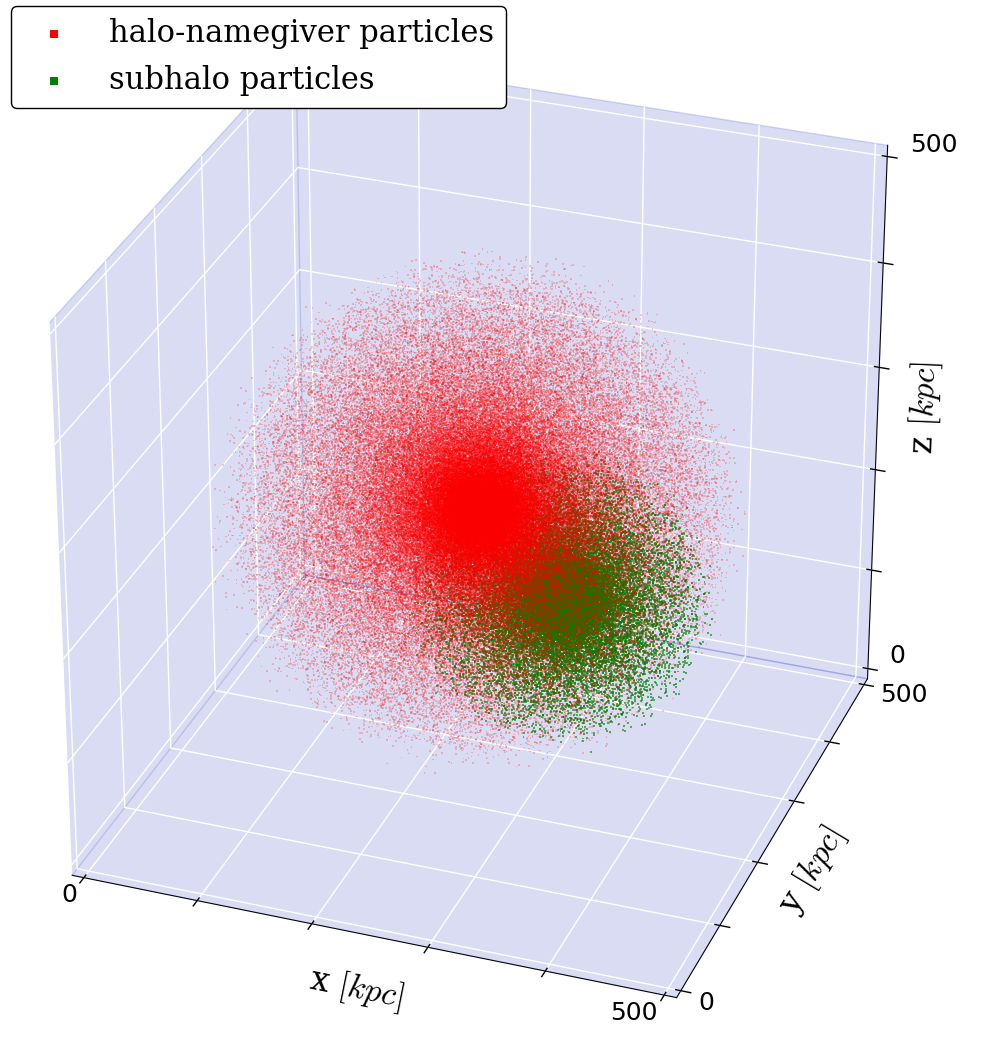
\includegraphics[height=\textwidth]{images/dice-two/dice-two-original-plot.png}}%
		\caption{
			The initial particle distribution of the \dt\ dataset. A smaller halo (subhalo 1) made of 40'000 particles is nested within a bigger halo (halo-namegiver), which contains 200'000 particles.
		}%
		\label{fig:dice_two_origin}
	\endminipage%\hspace{.1cm}
	\hspace*{\fill}
	%
	\minipage[t]{0.497\textwidth}
		\centering
		\fbox{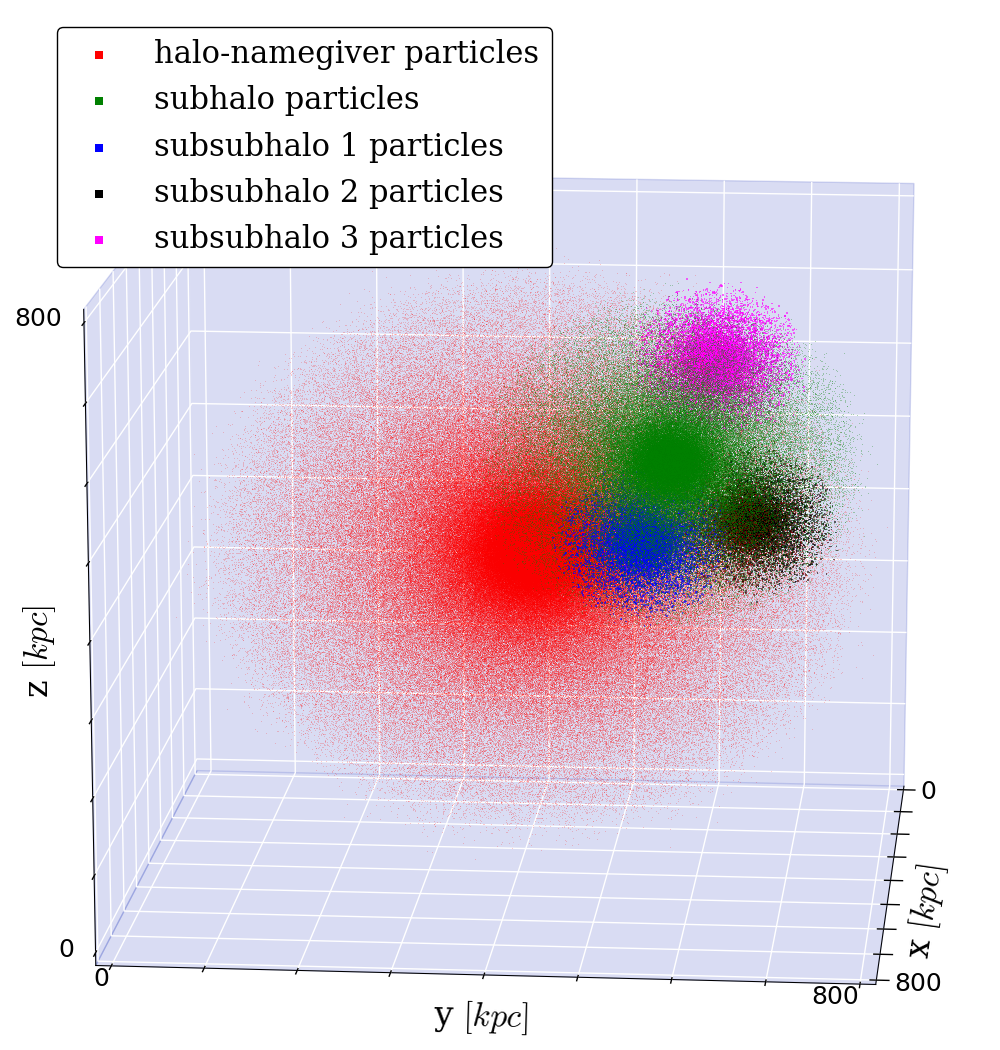
\includegraphics[height=\textwidth, keepaspectratio]{images/dice-sub/dice-sub-original-plot.png}}%
		\caption{
			The initial particle distribution of the \ds\ dataset. 3 small halos (subsubhalo 1-3), made of 20'000 particles, are around a bigger halo (subhalo 1), which contains 200'000 particles. These four structures are then enveloped by an even bigger halo (halo-namegiver), made of 1'000'000 particles.
		}%
		\label{fig:dice_sub_origin}
	\endminipage\hspace*{\fill} 
\end{figure}


%=======================
% DICE SUB
%=======================

The second test case created with \dice, the \ds\ dataset, consists of a halo made of 200'000 particles that has three subhalos, each containing 20'000 particles, following close Kepler orbits around it.
Then this composite structure is enveloped by an even bigger halo with 1'000'000 particles.
The purpose of this dataset is mainly to demonstrate the particle unbinding on a multi-levelled structure hierarchy.
The initial particle distribution is shown in figure \ref{fig:dice_sub_origin}.


%=======================
% COSMO
%=======================

The third dataset, named \cosmo, is a cosmological simulation, aiming to simulate very (physically) large structures and their formation over a long time interval. 
As such, it differs in multiple aspects to the previous two.
Firstly, the particles are described with comoving coordinates to account for the expansion of the Universe.
The computational domain is a cube (``\emph{box}'') of fixed length 1 that contains all the particles.
The physical coordinates of the particles at a certain time can then be computed with respect to the expansion scale factor at that time, thus implementing the expansion of the Universe without need to actually resize the box or move the particles at each time step solely because of the expansion.
Secondly, the simulation uses periodic boundary conditions. 
This means that if a particle would pass a surface of the box, it is reintroduced at the opposite surface.
The usage of periodic boundary conditions allows to simulate an infinite Universe by considering only a part of it and interpreting this part as representative of the entire Universe.
%This idea is justified by the cosmological principle, which states that at very large scales, the Universe is homogeneous and isotropic.
%``Large scales'' in this case are $\sim 100$ Mpc.
%Furthermore, by using periodic boundary conditions, the structures within the box are treated as if they weren't isolated, but influenced by structures outside the box.



The \cosmo\ dataset consists of $128^{3}$ $(\approx 2\cdot10^6)$ dark matter particles at redshift $z=0$ with the Hubble constant $H_0 = 70.4$ and density parameters $\Omega_m = 0.272$ and $\Omega_\Lambda=0.728$
\footnote{
	The density parameter of some cosmological component $i$ is defined as $\Omega_i  = \frac{\rho_i}{\rho_{crit}}$, where $\rho_i$ is its density and  $\rho_{crit}$ is defined as $\rho_{crit} = \frac{3 H^2}{8\pi G}$, where $H$ is the Hubble parameter and $G$ is the gravitational constant.
}.
The density threshold for clump finding was chosen to be 80 times the cosmological critical density $\rho_{crit}$  and the saddle threshold for halos was set to $200\rho_{crit}$.
Only halos with more that 10 particles were kept.
The particle distribution is shown in figure \ref{fig:cosmo_origin}.







\begin{figure}[!htb]
	\centering
	\fbox{\includegraphics[width = .8\textwidth ]{images/cosmo/cos-part2map-npart.png}}%
	\caption{
		The particle distribution of the \cosmo\ dataset.
		It is a cosmological simulation of $128^3$ dark matter particles at redshift $z=0$ with $H_0 = 70.4$ and density parameters $\Omega_m = 0.272$ and $\Omega_\Lambda=0.728$.
	}%
	\label{fig:cosmo_origin}
\end{figure}


	\section{Results}\label{chap:results}



%=====================
% Dice Two
%=====================

\subsection{Accuracy of the Potential in Dependance of the Number of Mass Bins}


Fig. \ref{fig:dice-two-binning} shows potentials computed with different numbers of mass bins, ranging from 10 to 10'000, and different binning distances (linear or logarithmic).
The potentials are computed for the subhalo of the \dt-dataset.
The results of 10'000 bins were taken as a reference point, which contain $\sim 5$ particles per bin on average.
Figure \ref{fig:dice-two-binning-analysis} shows the standard deviation $\sigma_N$ and the maximal deviation $D_{max,N}$ of the potential obtained with $N$ bins computed with
%Table \ref{tab:dice-two-binning-analysis} shows the total deviation $D_{tot,N}$ and the maximal deviation $D_{max,N}$ of the potential obtained with $N$ bins computed with
%
\begin{align}
	\sigma_N &= \left[ \frac{1}{N} \sum\limits_{i} \left( \frac{\phi(r_i)_N }{\phi(r_{i})_{10'000}} -1 \right)^2 \ \right] ^{\frac{1}{2}} \label{eq:Dtot} \\
	D_{max,N} &= \max \limits_{i} \left\{ \ \left | \frac{\phi(r_i)_N }{\phi(r_{i})_{10'000}} - 1 \right | \ \right\} \label{eq:Dmax}
\end{align}
%
where $r_{max}$ is the distance of the particle furthest away from the centre of mass ($r_{CoM}=0$ ). 
%$\phi(r_{max})$ is the potential at that distance, which is identical in all cases and for this reason used as a unit for the computation of the deviations.











\begin{figure}[!h]
	\centering
	\fbox{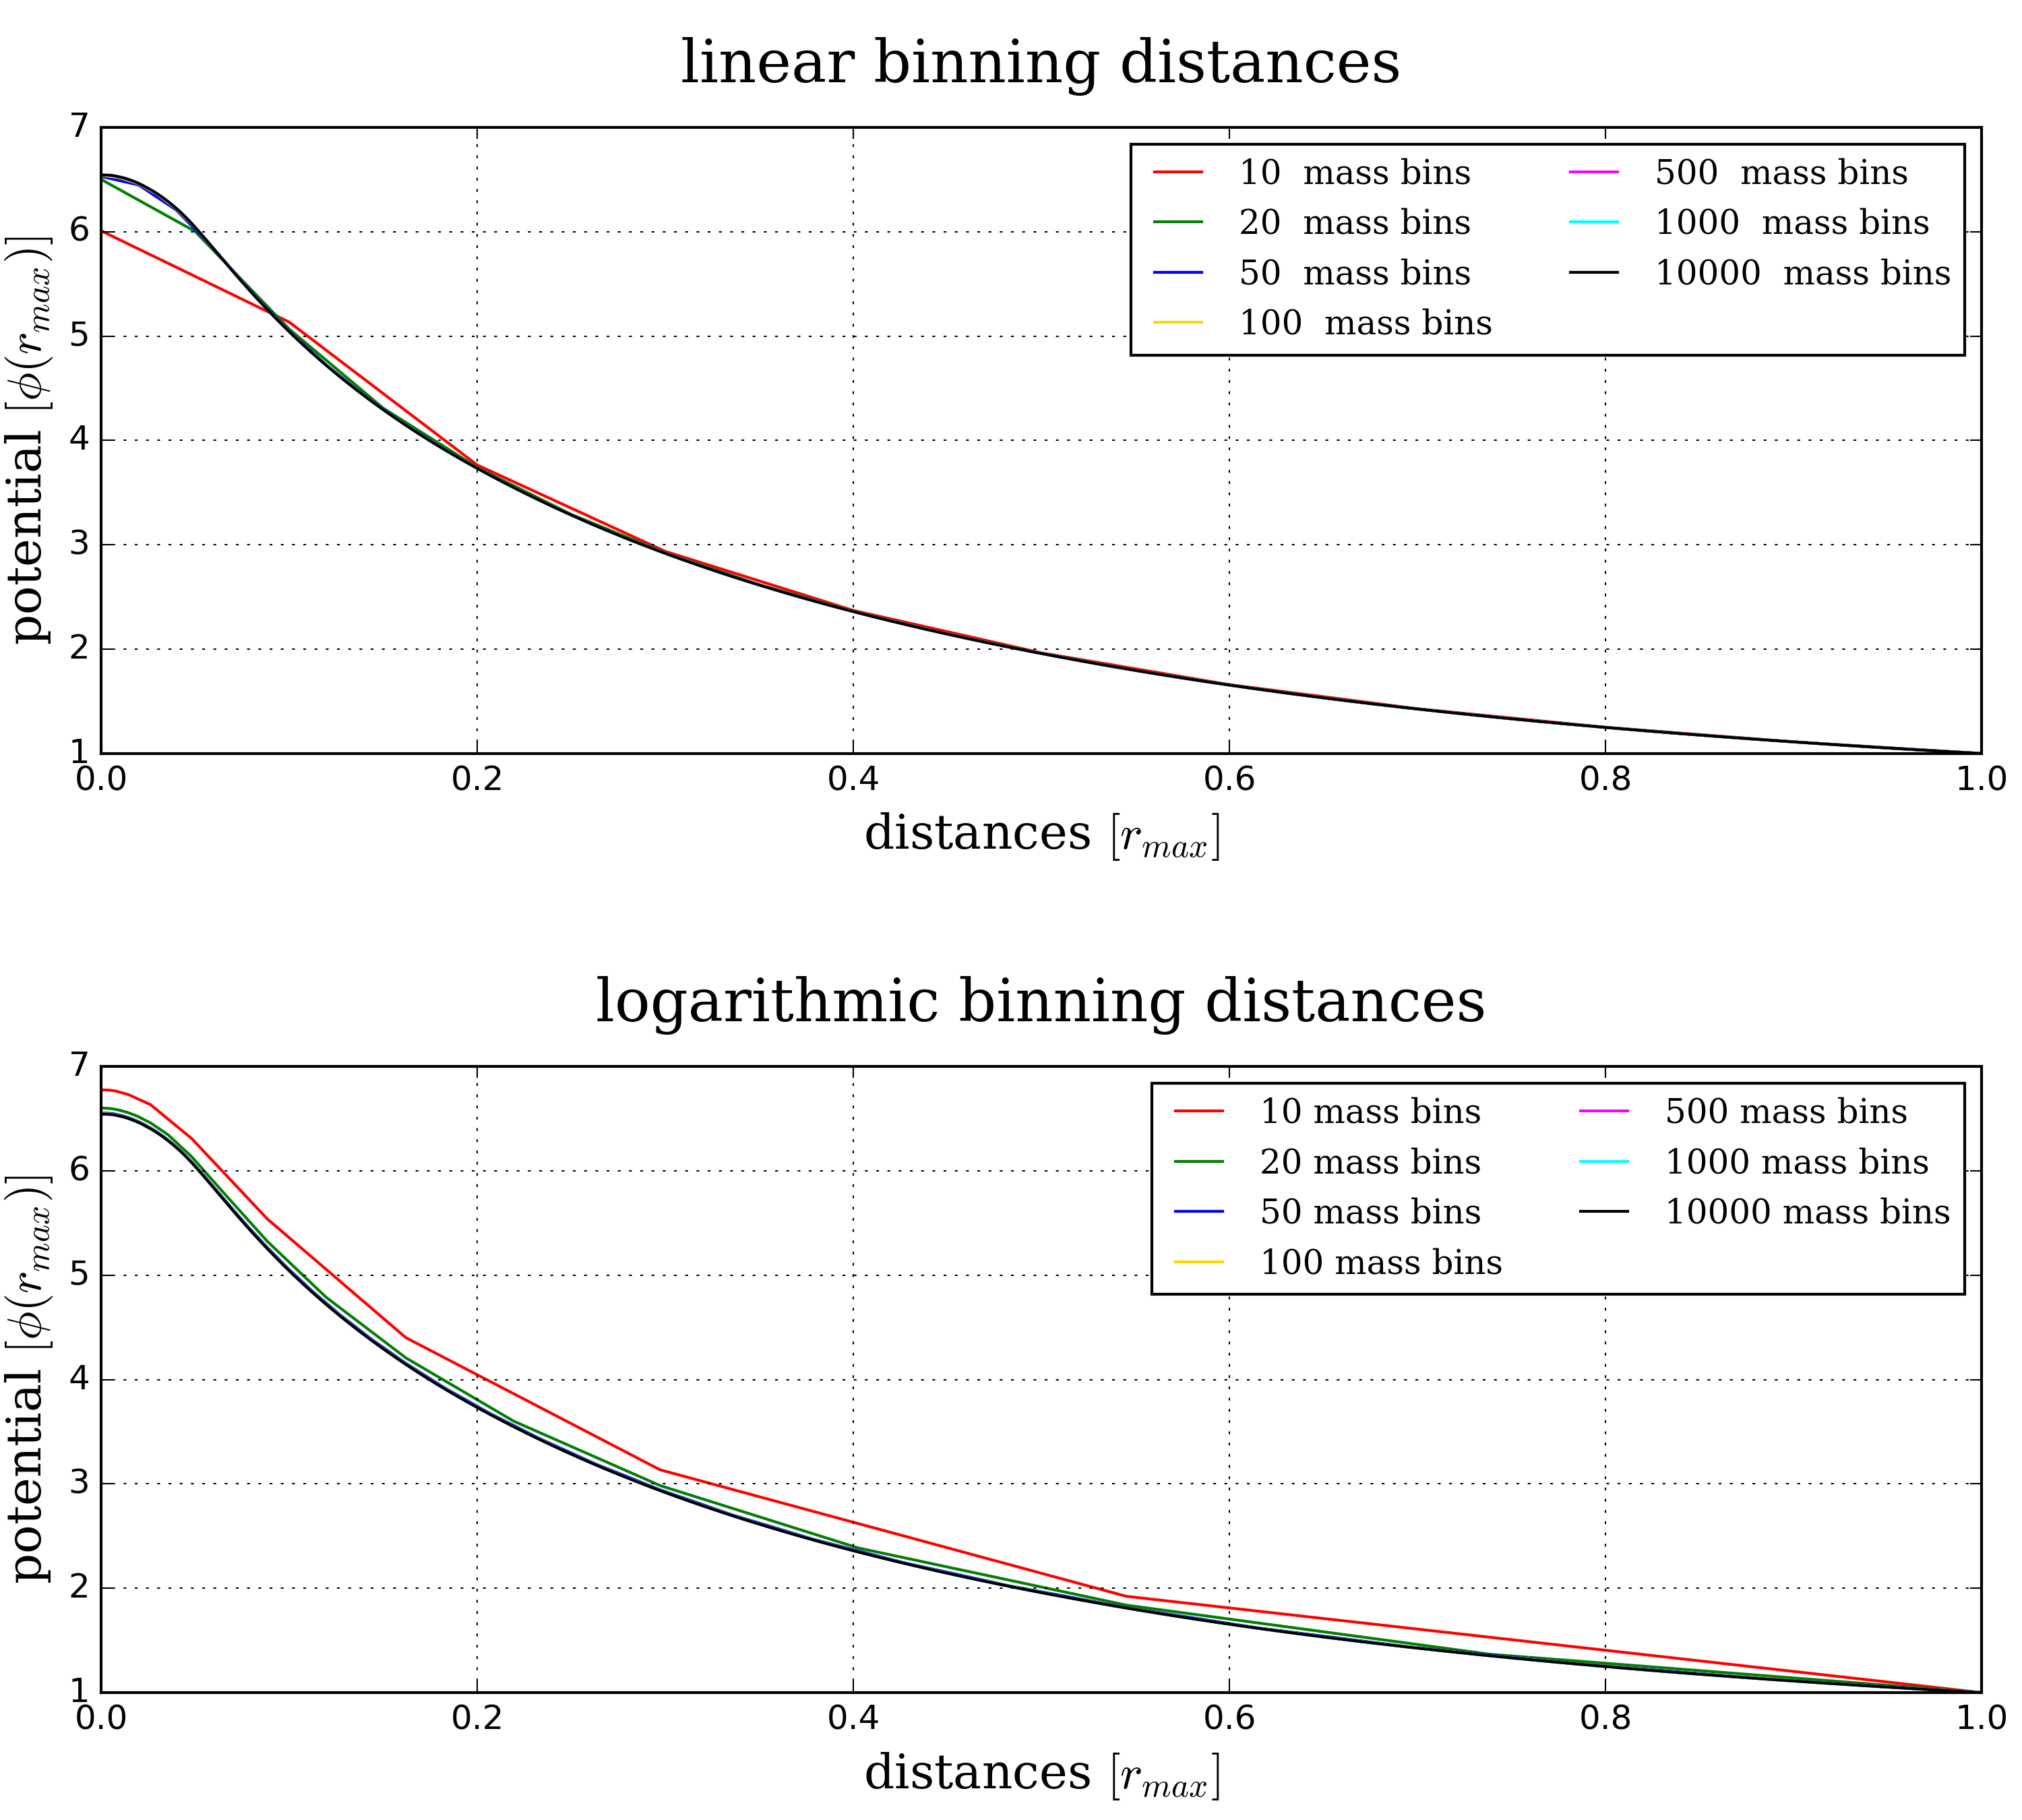
\includegraphics[width=.7\textwidth]{images/dice-two/phi_plot_4220_lin.png}}%
	\caption{
		The potential of the subhalo clump of the \dt-dataset computed with different binning methods and bin numbers.
		$r_{max}$ is the distance of the particle furthest away from the centre of mass, which is set at $r=0$
	}%
	\label{fig:dice-two-binning}
\end{figure}

\begin{figure}[!h]
	\centering
	\fbox{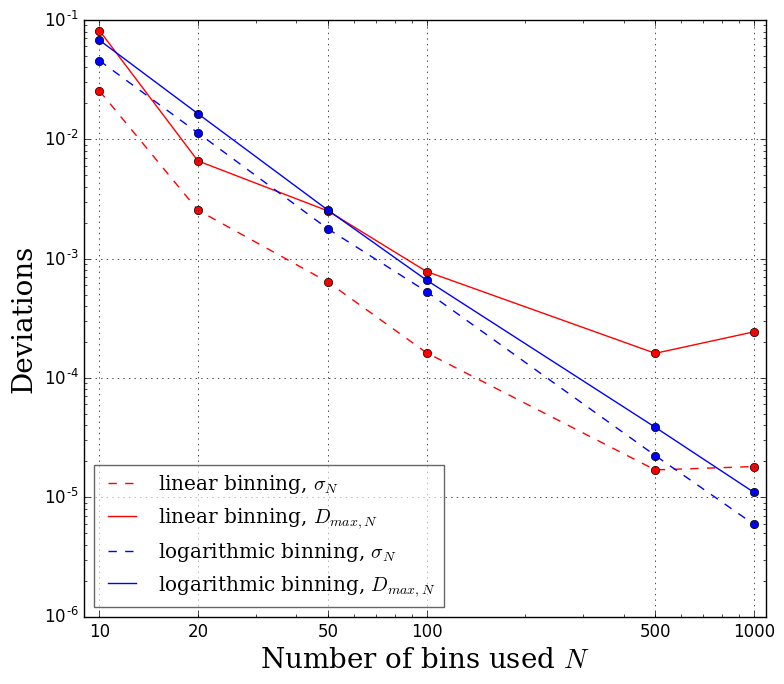
\includegraphics[width=.5\textwidth, keepaspectratio]{images/dice-two/phi_errors_plot_4220.png}}%
	\caption{ 
		Standard deviation $\sigma_N$ and maximal deviation $D_{max,N}$ of the potential obtained with $N$ bins, computed according to equations \ref{eq:Dtot} and \ref{eq:Dmax}, resp., for the subhalo clump of the \dt-dataset
	}%
	\label{fig:dice-two-binning-analysis}
\end{figure}








For both linear and logarithmic binning distances, the maximal deviation falls well below $1\%$ for 50 mass bins used, and below $0.1 \%$ for 100 mass bins.
Even though the standard deviation of linear binning is smaller for 100 bins, logarithmic bins are used for further tests because the logarithmic binning seems to describe the potential close to the centre of mass better.
This is particularly important when the unbinding includes iterative clump properties determination and considers neighbours, which will be shown in section \ref{chap:unbindings}.

Notably, the potential obtained with 10 bins and logarithmic binning distances seems to be the only one deviating on every point.
This is caused by the way the integral for the potential is computed:
%The computation of the integral is always between two bins.
As the bin widths grow for logarithmic binning distances, the accuracy decreases.
The error for 10 bins and logarithmic binning distances should be the highest of all.
Once the integral of each bin is computed, the integral is then summed up beginning at the outermost bin with respect to the centre of mass, so a large error at the first bin will propagate through every other bin. 





















\subsection{Effect of Iterative Clump Properties Determination}\label{chap:iter}

\begin{table}[!htb]
	\begin{centering}
		\begin{tabular}[t]{|r | l | r | l |}
			\hline
			$\varepsilon$     &       $d_v$ 	& \texttt{niter}  		&	$D_v$	\\
			\hline
			0.5       &        0.3000  	&  		 		2    	&	0.2326  \\
			0.1       &        0.0614  	&           	4    	&	0.0419	\\
			0.01      &        0.0036  	&           	7    	&	0.0024	\\
			0.001     &        0.0010  	&           	8    	&	0.0014  \\       
			0.0001    &        0.0000  	&          		10    	&	0.0009 	\\
			\hline
		\end{tabular}
	\caption{%
			The deviation $D_v$ (eq. \ref{eq:Dv}) from the originally set bulk velocity to the computed bulk velocity for the subhalo of the \dt-dataset in dependence of the convergence limit $\varepsilon$.
			The iterative clump properties determination halts after \texttt{niter} iterations, when the difference $d_v$ of the previously determined bulk velocity to the new bulk velocity, $d_v = \frac{v_{bulk} - v_{bulk,old}}{v_{bulk,old}} < \varepsilon$.
	}
	\label{tab:converging}%
	\end{centering}
\end{table}


For the \dt-dataset, the precise relative velocity of the two clumps is known.
Table \ref{tab:converging} shows the deviation $D_v$ of the computed clump bulk velocity $v_{bulk}$ from the original bulk velocity $v_{orig}$ as set with \dice\ with decreasing converging limits $\varepsilon$.
$D_v$ is computed as follows:
%
\begin{align}
	D_v = \left | 	 \frac{v_{bulk} - v_{orig}}{v_{orig}}				\right | \label{eq:Dv}
\end{align} 
%
The deviation falls below $1\%$ for $\varepsilon = 0.01$, which is why that value will be used for further tests.






















\subsection{Effects of Different Unbinding Methods}\label{chap:unbindings}

Taking neighbouring structures into account and determining clump properties iteratively are attempts to improve the accuracy of the particle unbinding, but can be left out if desired.
In this section, the results of three different unbinding methods on the three previously introduced datasets as well as the results as found by the clump finder without unbinding.
The methods are named as follows:
%
%{\centering
%	\begin{tabular}[c]{l p{13cm}}
%		\simple	&	Simple unbinding without considering neighbour clumps for the potential nor determining clump properties iteratively.\\
%		\neigh	& 	Unbinding considering neighbour clumps for the potential \\%as described in section \ref{chap:neighbours} \\
%		\iter	&	Unbinding considering neighbour clumps for the potential and iterative clump properties determination% as described in section \ref{chap:iter_theory}
%	\end{tabular}
%}
\begin{labeling}{\texttt{neighbours}}
	\renewcommand{\arraystretch}{0.1}
 	\item [\simple]		Simple unbinding without considering neighbour clumps for the potential nor determining clump properties iteratively.
	\item [\neigh]		Unbinding considering neighbour clumps for the potential
	\item [\iter]		Unbinding considering neighbour clumps for the potential and iterative clump properties determination
\end{labeling}

%
All three unbinding methods are executed with 100 mass bins and logarithmic binning distances.
For the \iter\ runs, the convergence limit $\varepsilon$ was set to 0.01.
The results without particle unbinding, which are the results as found by \phew, are also the initial situation on which the unbinding is performed.
They are labelled as ``\phewon''.

Table \ref{tab:unbinding_results} shows the number of particles in clumps for these unbinding methods.
For the \cosmo-dataset, all halo-namegiver and subhalo particles have been summed up respectively, because there were too many clumps ($\sim 19'000$) to represent individually.
Furthermore, the particle distributions for all four runs and all three datasets are shown in figures \ref{fig:dice_two_results}, \ref{fig:dice_sub_results} and \ref{fig:cosmo_results}.
In case of the \cosmo-dataset, only one halo and its substructure are shown instead all of them simultaneously, so the effects of the unbinding methods can be seen better.
%There are three plots for each of the four runs: The first contains all particles, the second only the halo-namegiver clump particles, and the last one only the substructure particles.

\begin{table}[!htb]
	{\footnotesize
	\begin{centering}
		\def\arraystretch{1.2}
		\begin{tabular}[t]{ l | R{2.5cm} |  R{2.5cm} |  R{2.5cm} |  R{2.5cm} |}
			%
			%=======================
			% DICE TWO 
			%=======================
			%
			\cline{2-5}
							& \multicolumn{4}{|c|}{\textbf{\dt-dataset}} \\
			\cline{2-5}
							& \phewon    &  \simple & \neigh  & \iter \\
			\hline
			\hline
			halo-namegiver particles 	&	187606	&	202998	& 233450		&	231905	\\
			subhalo particles 			&	52394	&	37002	&	6550	&	8095	\\
			\hline
			\multicolumn{5}{c}{}\\
			%
			%
			%
			%=======================
			% DICE SUB 
			%=======================
			%
			\cline{2-5}
				& \multicolumn{4}{|c|}{\textbf{\ds-dataset}} \\
			\cline{2-5}
				& \phewon    &  \simple & \neigh  & \iter \\
			\hline
			\hline
			halo-namegiver particles 	&	965485	& 	975038	& 1196614	&	1180544	\\
			subhalo particles 			&	197767	&	221977	&	49647	&	58963	\\
			subsubhalo 1 particles 		&	38734	&	23398	&	4475	&	7280	\\
			subsubhalo 2 particles 		&	26591	&	19590	&	5239	&	6151	\\
			subsubhalo 3 particles 		&	31421	&	19995	&	4023	&	7060	\\
			\hline
			\multicolumn{5}{c}{}\\
			%
			%
			%
			%
			%=======================
			% COSMO 
			%=======================
			%
			\cline{2-5}
				& \multicolumn{4}{|c|}{\textbf{\cosmo-dataset}} \\
			\cline{2-5}
				& \phewon    &  \simple & \neigh  & \iter \\
			\hline
			\hline
			halo-namegiver particles 	&	573832	&	640686	&	746441	&	740616	\\
			subhalo particles 			&	188036	&	121182	&	15427	&	21252	\\
			\hline
			\multicolumn{5}{c}{}\\
			%
			%
		\end{tabular}
	\end{centering}
	} %footnotesize
	\caption{%
		The number of particles in clumps depending on the unbinding method for the \dt-, \ds- and \cosmo-dataset.
	}%
	\label{tab:unbinding_results}%
\end{table}


%The effects of the different unbinding methods can be seen very well in the images and the table.
Comparing the results of \phew\ and the \simple\ unbinding of the \dt-dataset in figure \ref{fig:dice_two_results_a} and of the \cosmo-dataset in figure \ref{fig:cosmo_results_a} shows that the \simple\ method already has a decent contribution to the assignment of particles to the structures.
Looking at the halo-namegiver particles only, one can see that where \phew\ has made clean cuts between the clumps, now particles have been re-introduced, yielding smoother structures.

The results of the \simple\ unbinding for the \ds-dataset in fig. \ref{fig:dice_sub_results_a} and table \ref{tab:unbinding_results} show clearly that most unbound particles from the lowest level substructure, the subsubhalos, have been assigned to the parent clump, not to the halo-namegiver.
Note for example that most substructure particles above the subsubhalo 1 (green) are assigned to the subhalo (pink) after \simple\ unbinding.
The surfaces of the subsubhalos facing away from the subhalo appear much more spherical, which is how they were originally created to be.


In all three figures, the effect of considering neighbours for the potential seems drastic.
But recall that when neighbouring clumps are considered for the potential, the particles that remain after unbinding are exclusively bound to the subhalo they are assigned to.
The substructure clumps have indeed been stripped from most of their particles and only what appears to be ``cores'' close to the centre of mass remain, in agreement with what one would expect considering the argumentation used in context with figures \ref{fig:orbits} and \ref{fig:potentials}. 
%This was to be expected, it is in agreement with figure \ref{fig:orbits} that only particles close to the centre of mass will be bound exclusively to the subhalos.
Two subhalos from the halo of the \cosmo-dataset (figure \ref{fig:cosmo_results}, subhalo 1 and 5, have even been stripped of all their particles, indicating that none of their particles can be considered as exclusively bound to them.



The iterative determination of clump properties seems to find overall more bound particles compared to the \neigh\ runs.
In each of the presented cases the total number of particles in substructure grew.
In case of the \cosmo-dataset, 36 clumps had less bound particles (472 particles in total) after \iter-unbinding, while 187 clumps had more bound particles, 6297 in total.


Unfortunately, iterative clump properties determination couldn't re-introduce any particles to the completely unbound subhalos 1 and 5 of the halo shown in fig. \ref{fig:cosmo_results_b}. 
If all particles are unbound at the first iteration already, no new clump properties can be determined and the situation remains as it is.
If necessary, an attempt to improve on this effect might be to first determine clump properties iteratively for such cases and only after the iteration has finished take neighbouring structures into account.
This feature has not been adapted, as no urgent need for it was seen.
It is perfectly plausible that some substructure as identified by \phew\ could contain no exclusively bound particles. 




%=====================
% Dice Two
%=====================

\begin{subfigures}
	\begin{figure}[!htbp]
		{
		\renewcommand{\arraystretch}{0.1}		
		\centering	
	%	\subfloat[]{
		\begin{tabular}{|p{.5cm} c c|}
			\hline
			&&\\[1em]
			&	\phewon\ 	& \simple \\[1.5em]
			%
			%
			\begin{sideways}{\hspace{3cm} \textbf{All particles}}\end{sideways} \hspace*{-1em}	&		 
			{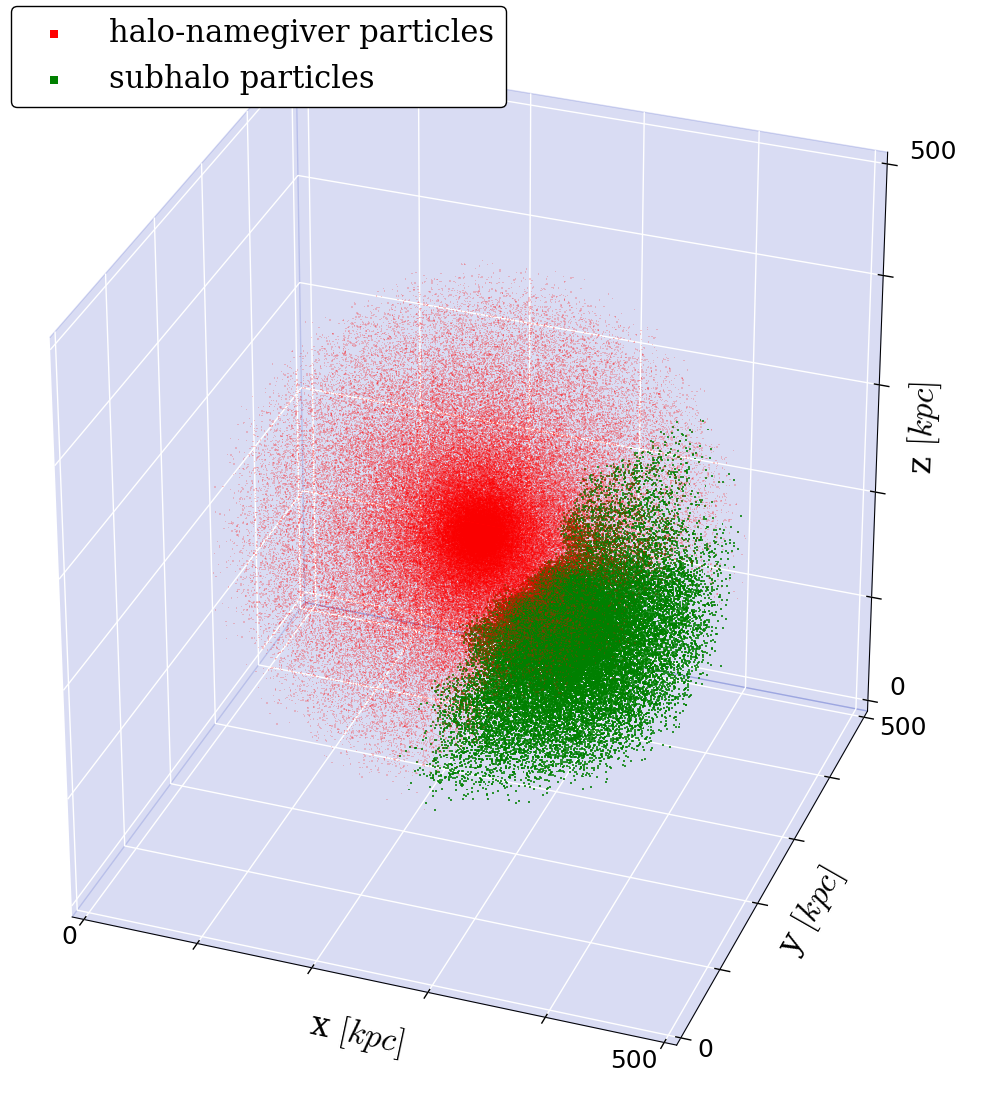
\includegraphics[width = .42\textwidth]{images/dice-two/dice-two-plot-halo1451-phew.png}} \hspace*{-1em} 	& 
			{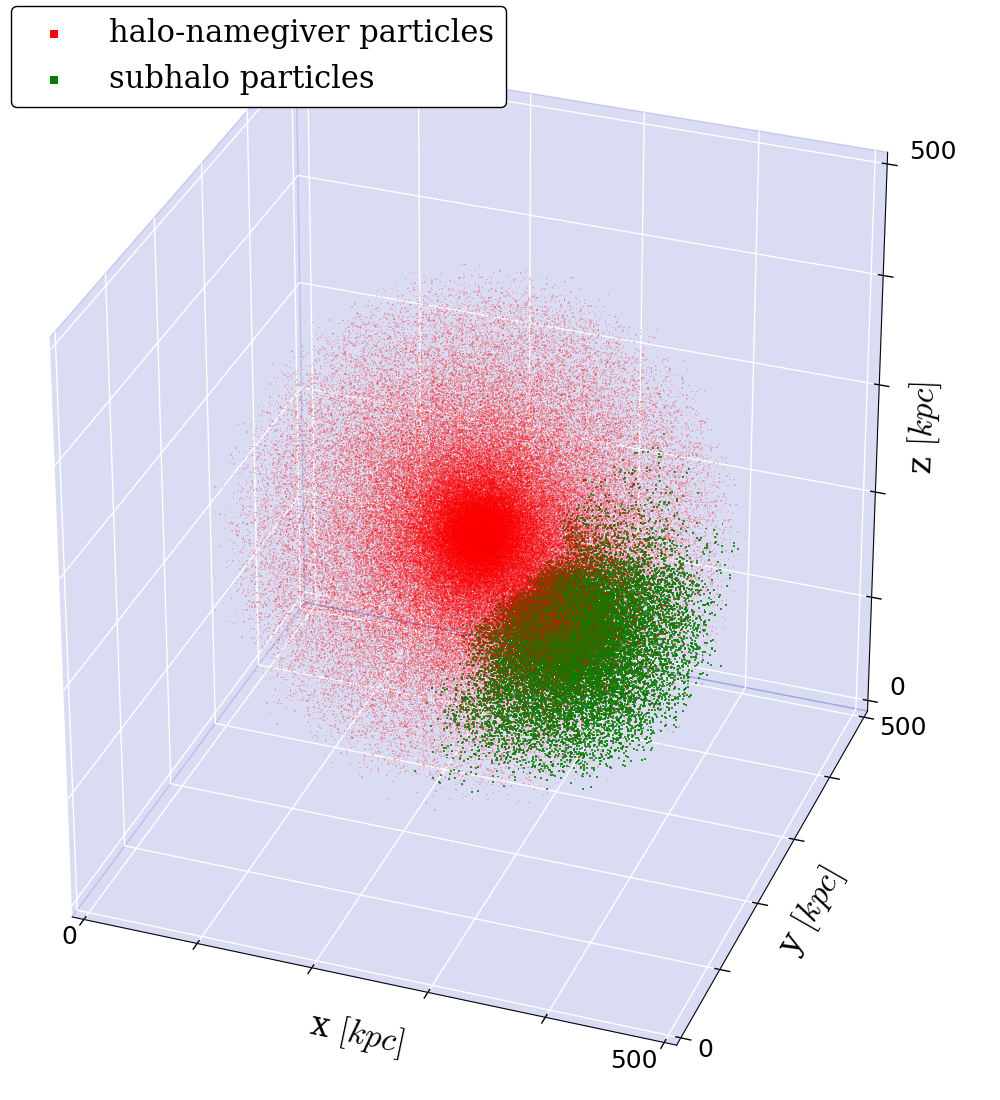
\includegraphics[width = .42\textwidth]{images/dice-two/dice-two-plot-halo1451-nosaddle.png}} \hspace*{-1em}	\\
			%
			%
			\begin{sideways}{ \hspace{.5cm}\textbf{Halo-namegiver particles only} }\end{sideways}	 \hspace*{-1em}			 &			 
			{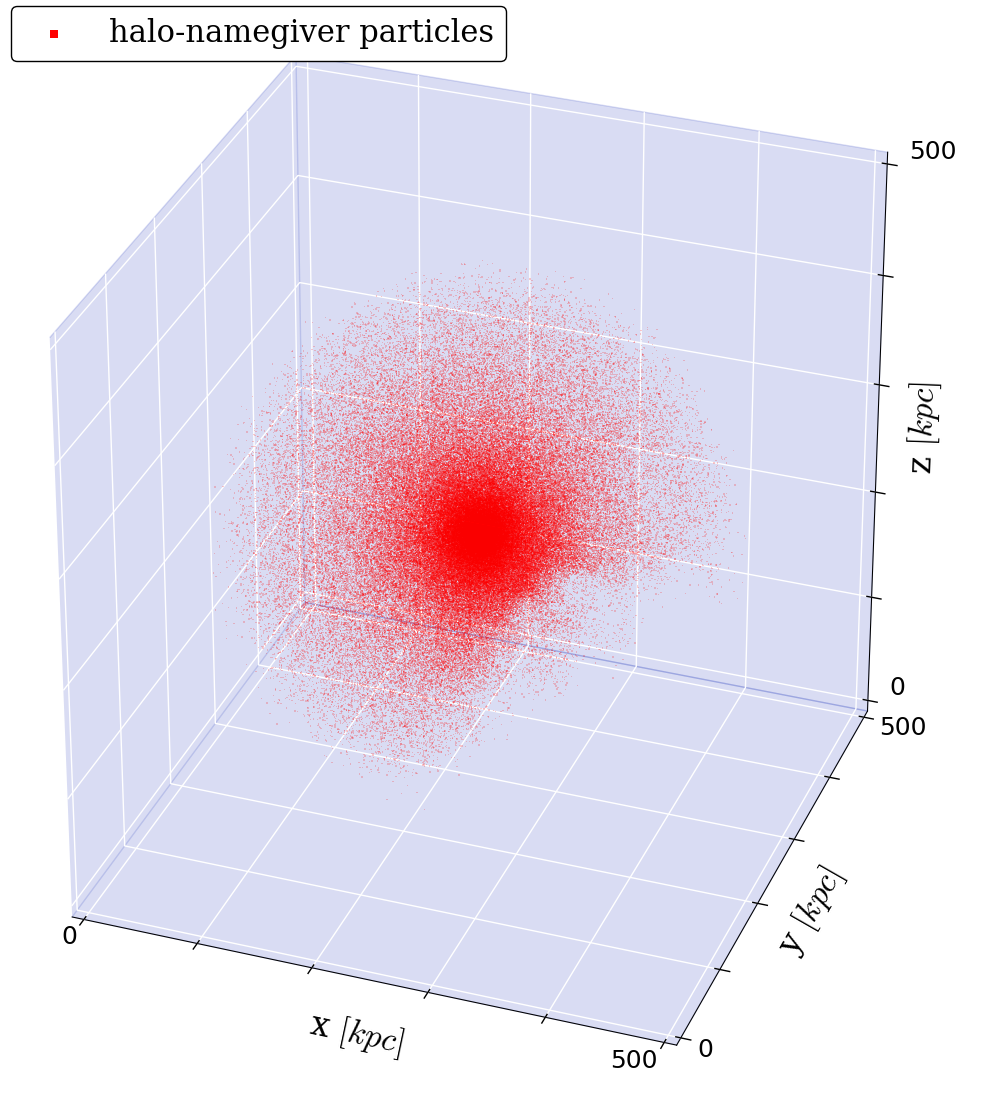
\includegraphics[width = .42\textwidth]{images/dice-two/dice-two-halo-only-phew.png}} \hspace*{-1em} 		&
			{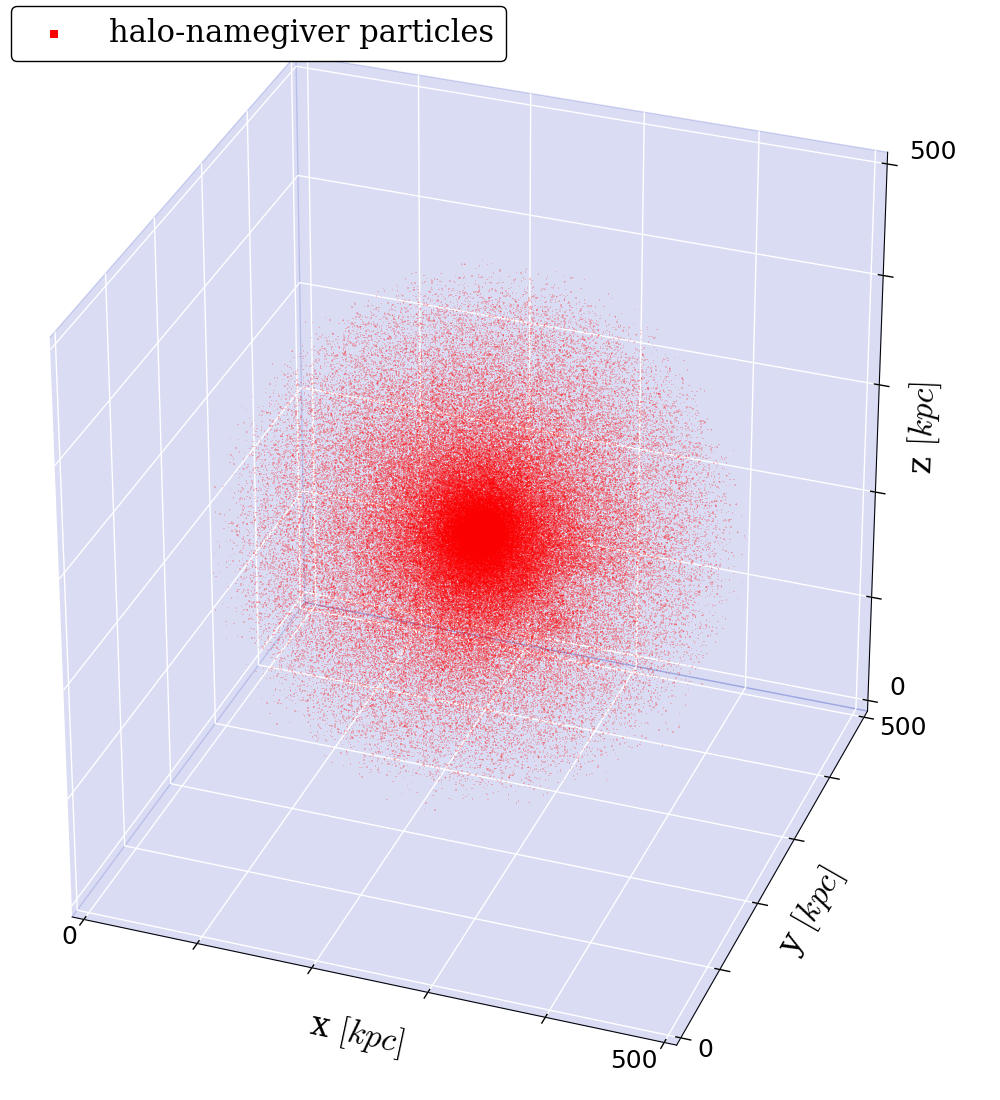
\includegraphics[width = .42\textwidth]{images/dice-two/dice-two-halo-only-nosaddle.png}} \hspace*{-1em}		\\
			%
			%
			\begin{sideways}{ \hspace{2cm}\textbf{Subhalo particles only} }\end{sideways}	 \hspace*{-1em}			 &
			{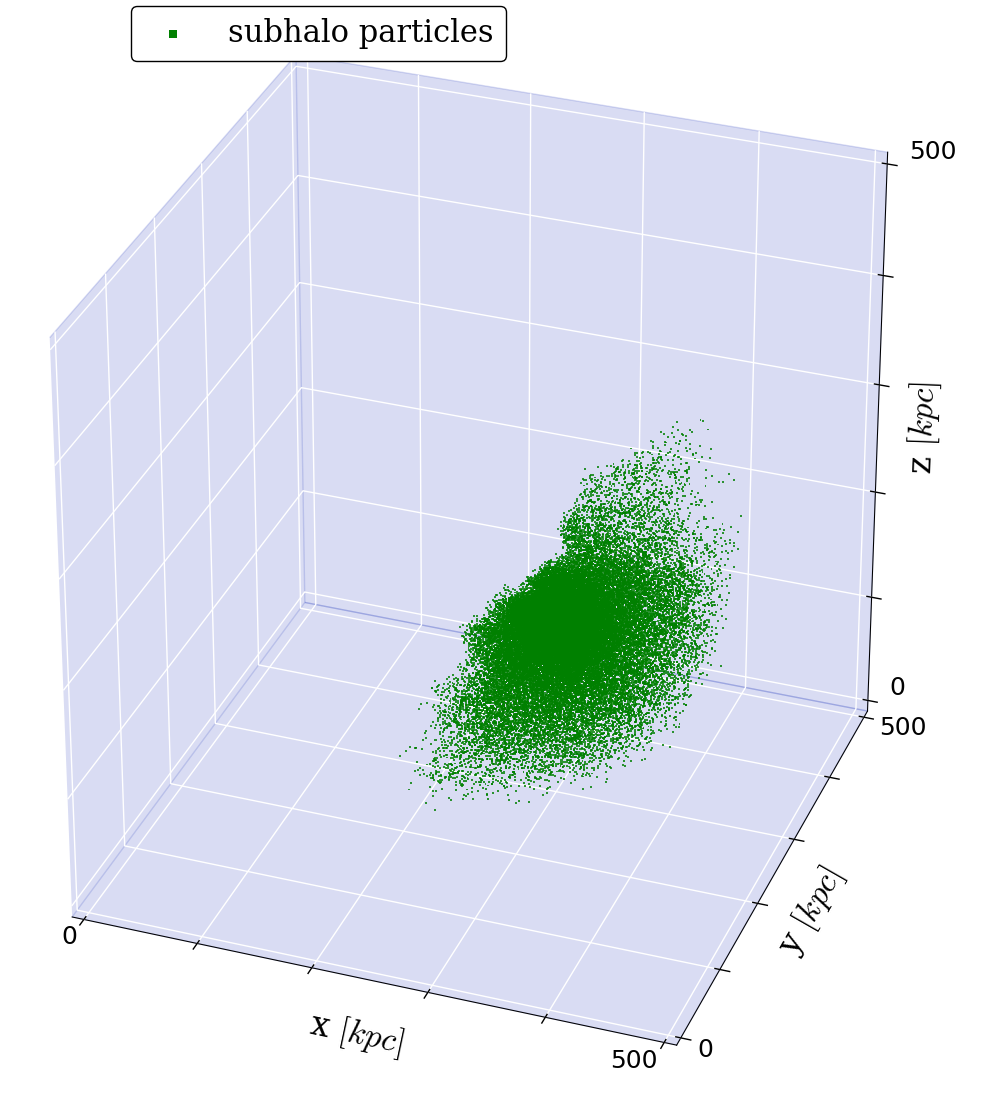
\includegraphics[width = .42\textwidth]{images/dice-two/dice-two-plot-subhalo-phew.png}} &
			{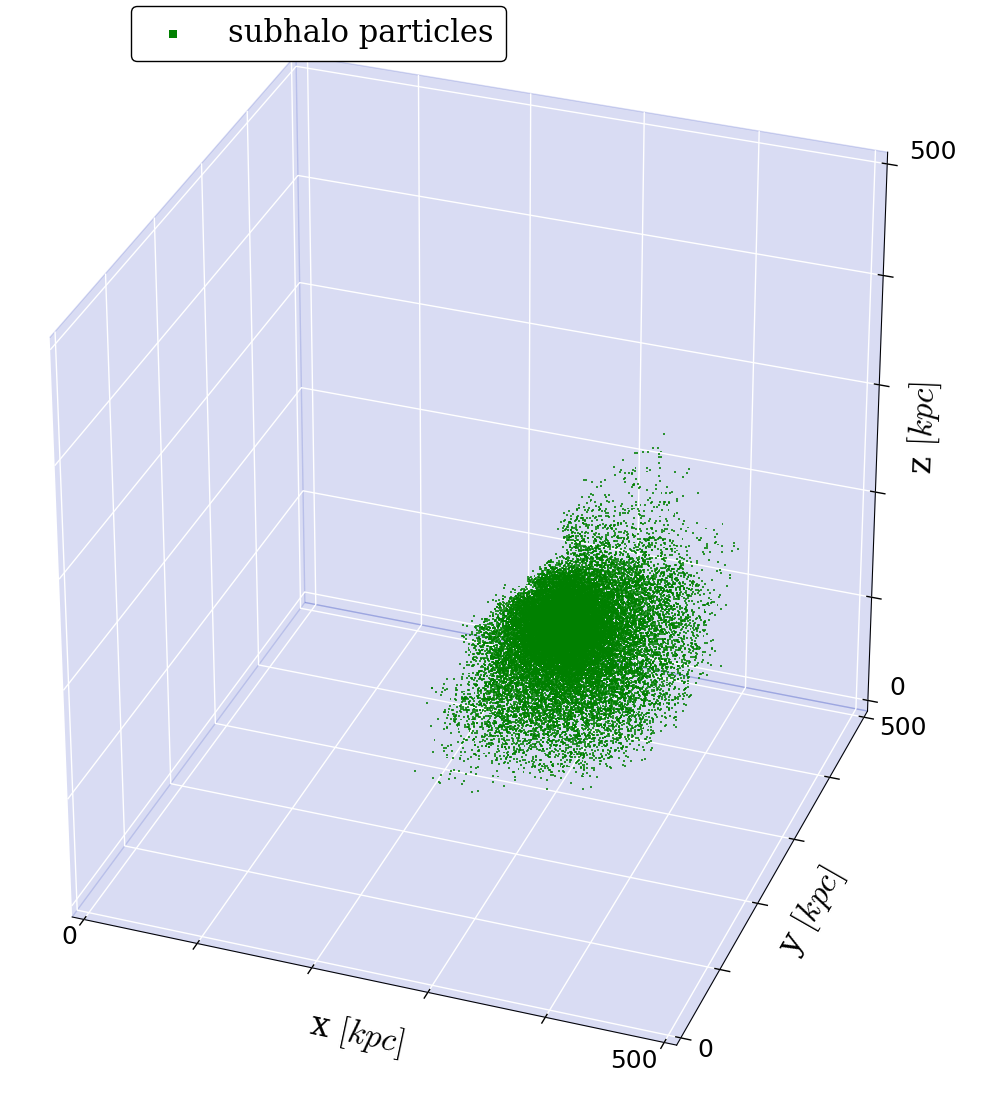
\includegraphics[width = .42\textwidth]{images/dice-two/dice-two-plot-subhalo-nosaddle.png}} \\
			\hline
		\end{tabular}
		\caption{\label{fig:dice_two_results_a}The results of \phewon\ and \simple\ unbinding of the \dt-dataset: All particles, halo-namegiver particles only and subhalo particles only.}
		}
	\end{figure}
%=================================================
%=================================================
%=================================================
	\begin{figure}[!htbp]%\ContinuedFloat
		{
		\renewcommand{\arraystretch}{0.1}
		\centering	
		\begin{tabular}{|p{.5cm} c c|}
			\hline
			&&\\[1em]
			&	\neigh\ 	& \iter \\[1.5em]
			%
			%
			\begin{sideways}{\hspace{3cm} \textbf{All particles}}\end{sideways} \hspace*{-1em}	&		 
			{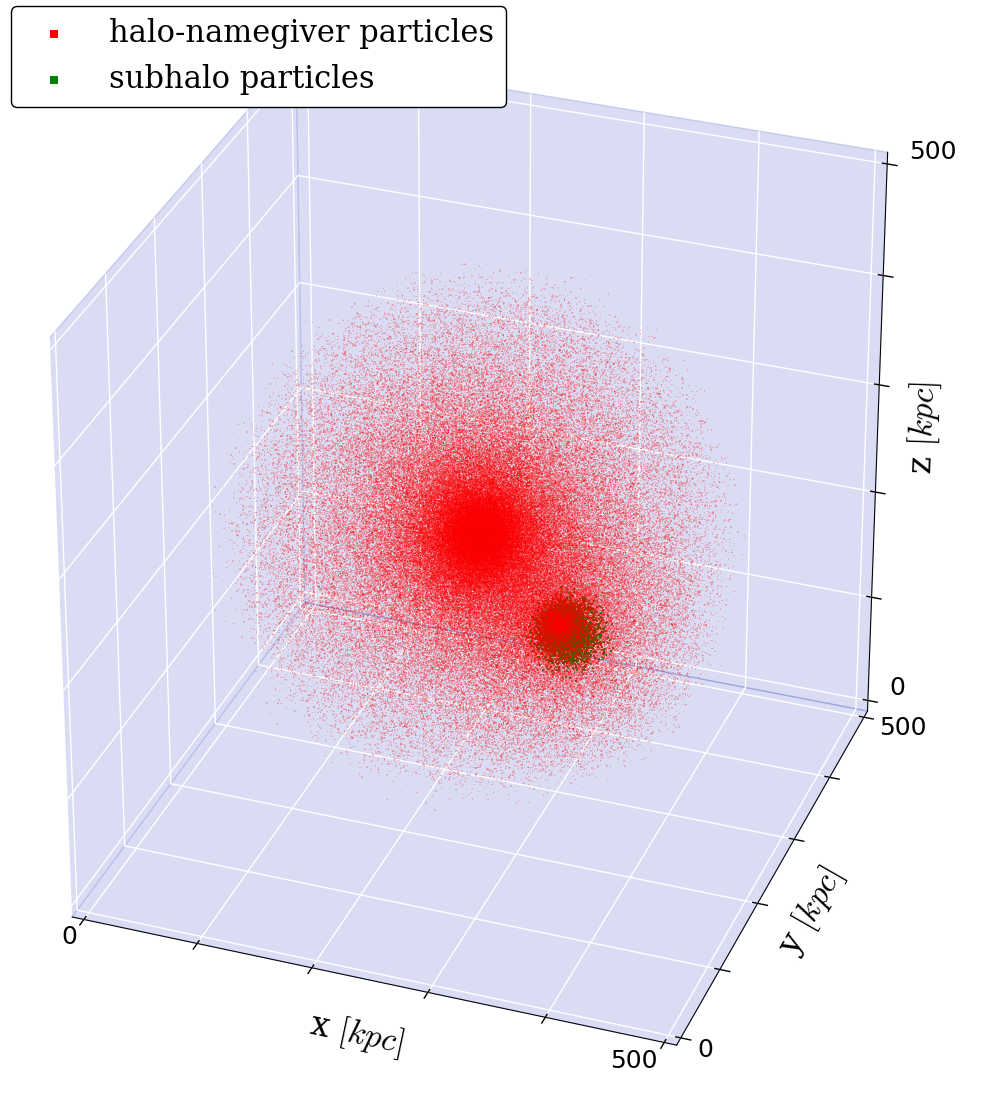
\includegraphics[width = .42\textwidth]{images/dice-two/dice-two-plot-halo1451-saddle.png}} \hspace*{-1em} 	& 
			{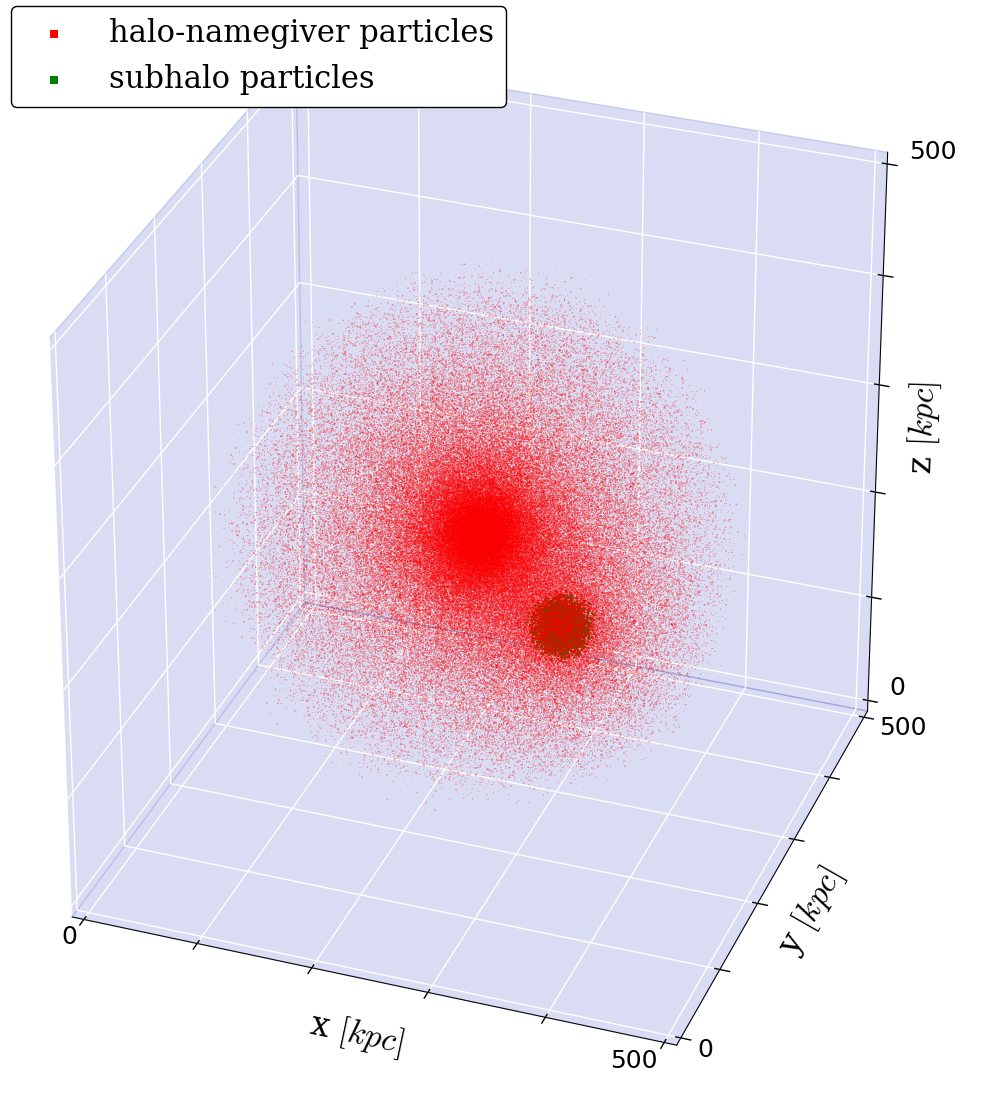
\includegraphics[width = .42\textwidth]{images/dice-two/dice-two-plot-halo1451-iter.png}} \hspace*{-1em}	\\
			%
			%
			\begin{sideways}{ \hspace{.5cm}\textbf{Halo-namegiver particles only} }\end{sideways}	 \hspace*{-1em}			 &			 
			{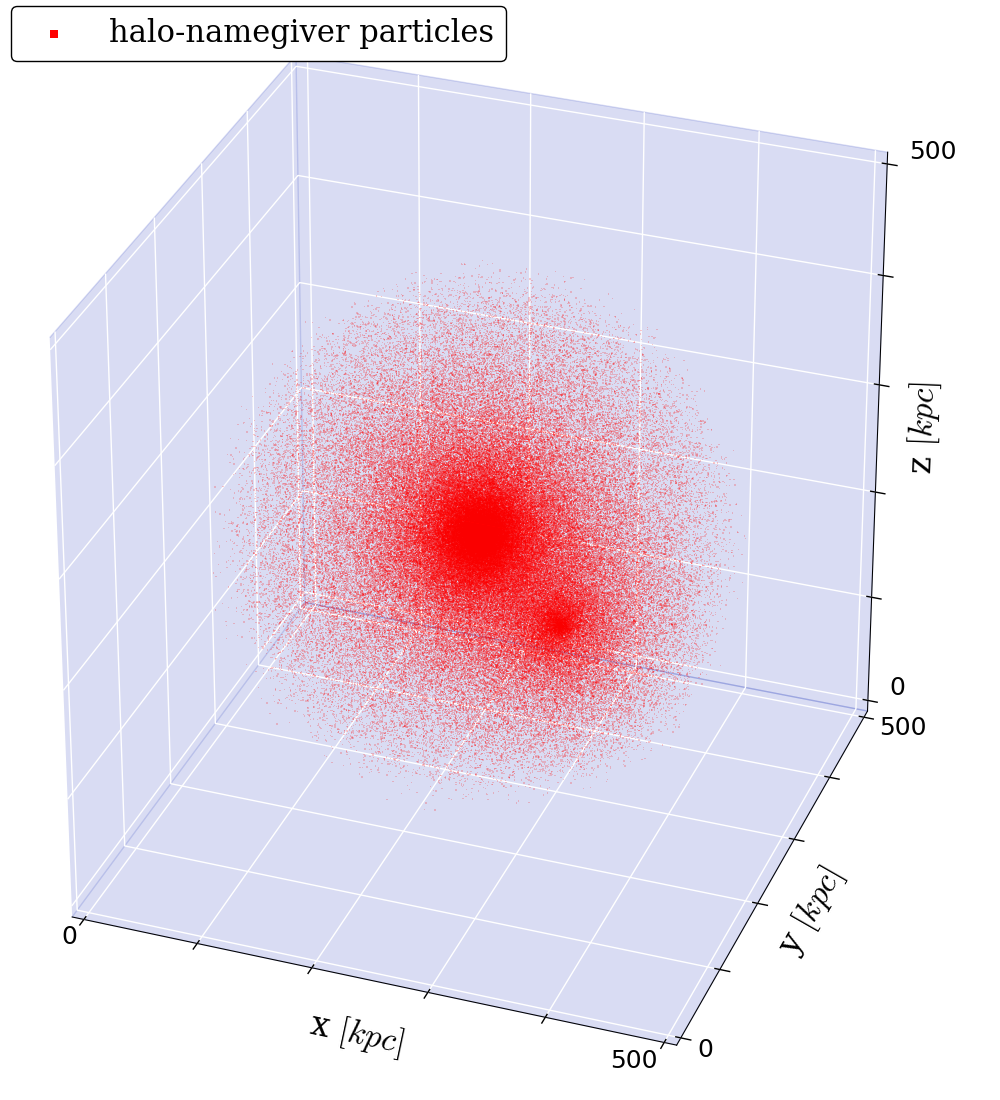
\includegraphics[width = .42\textwidth]{images/dice-two/dice-two-halo-only-saddle.png}} \hspace*{-1em} 		&
			{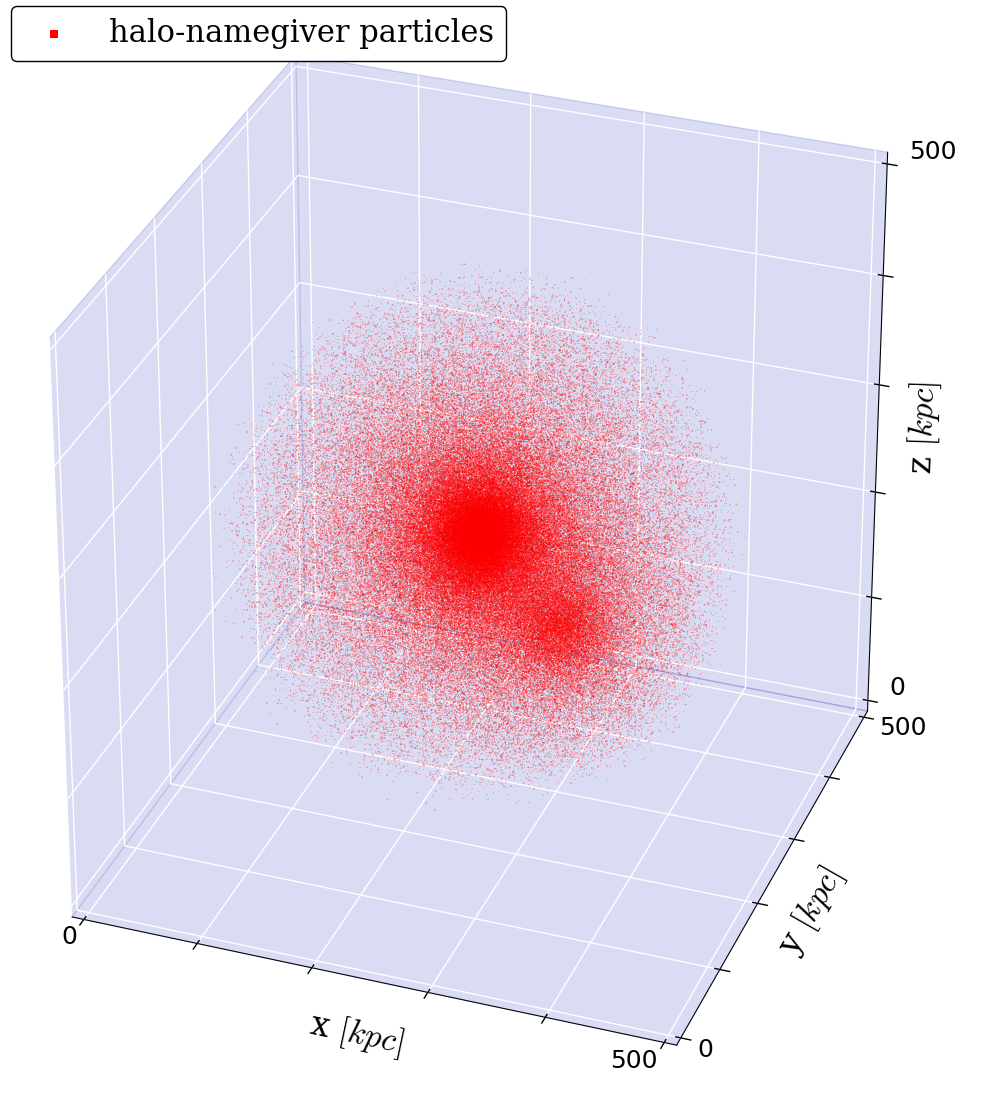
\includegraphics[width = .42\textwidth]{images/dice-two/dice-two-halo-only-iter.png}} \hspace*{-1em}		\\
			%
			%
			\begin{sideways}{ \hspace{2cm}\textbf{Subhalo particles only} }\end{sideways}	 \hspace*{-1em}			 &
			{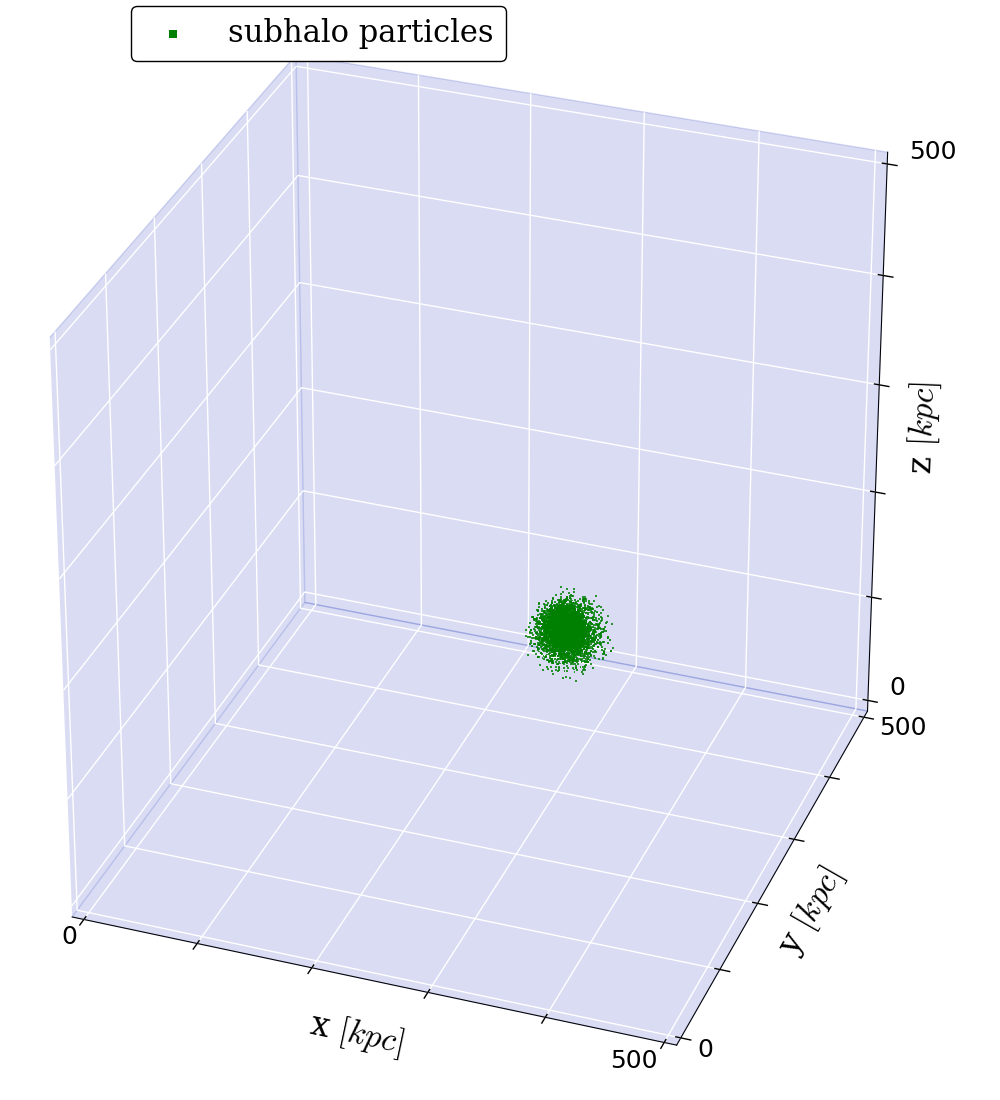
\includegraphics[width = .42\textwidth]{images/dice-two/dice-two-plot-subhalo-saddle.png}} &
			{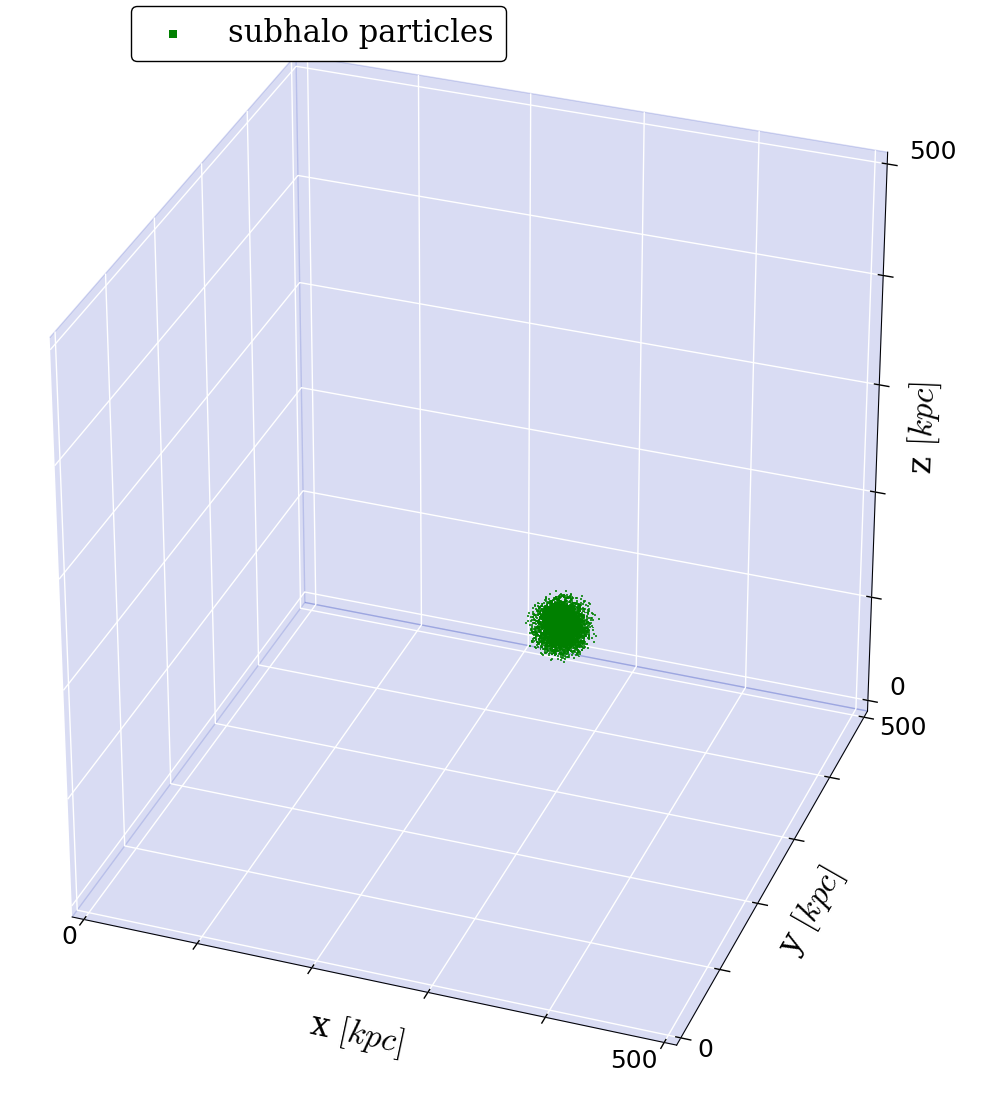
\includegraphics[width = .42\textwidth]{images/dice-two/dice-two-plot-subhalo-iter.png}} \\
			\hline
		\end{tabular}
		\caption{\label{fig:dice_two_results_b}
			The results of \neigh\ and \iter\ unbinding of the \dt-dataset: All particles, halo-namegiver particles only and subhalo particles only.
			}
		}
	\end{figure}
	\label{fig:dice_two_results}
\end{subfigures}







%=====================
% Dice Sub
%=====================

\begin{subfigures}

	\begin{figure}[!htbp]
		{
			\renewcommand{\arraystretch}{0.1}
			\centering	
			%	\subfloat[]{
			\begin{tabular}{|p{.5cm} c c|}
				\hline
				&&\\[1em]
				&	\phewon\ 	& \simple \\[1.5em]
				%
				%
				\begin{sideways}{\hspace{3cm} \textbf{All particles}}\end{sideways} \hspace*{-1em}	&		 
				{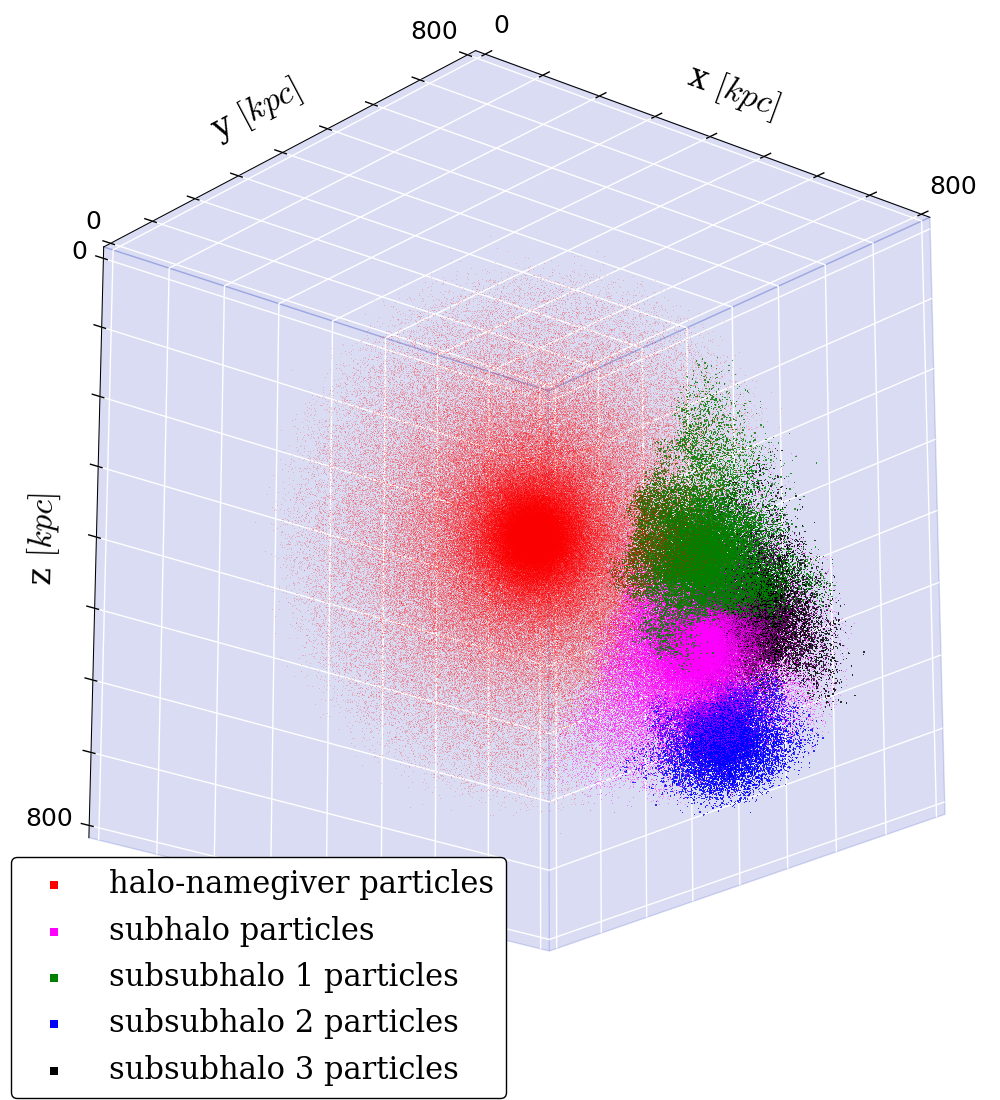
\includegraphics[width = .42\textwidth]{images/dice-sub/dice-sub-plot-halo1-phew.png}} \hspace*{-1em} 	& 
				{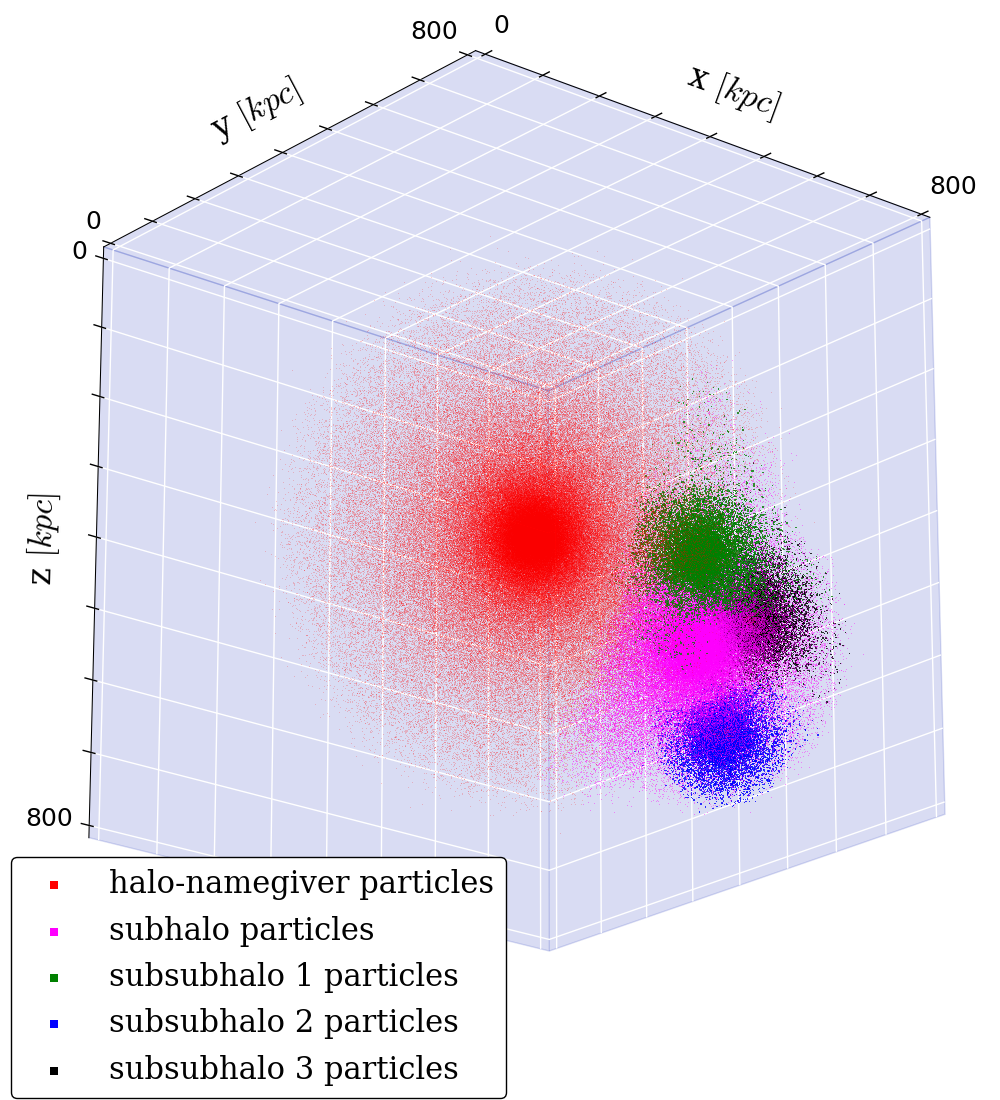
\includegraphics[width = .42\textwidth]{images/dice-sub/dice-sub-plot-halo1-nosaddle.png}} \hspace*{-1em}	\\
				%
				%
				\begin{sideways}{ \hspace{.5cm}\textbf{Halo-namegiver particles only} }\end{sideways}	 \hspace*{-1em}			 &			 
				{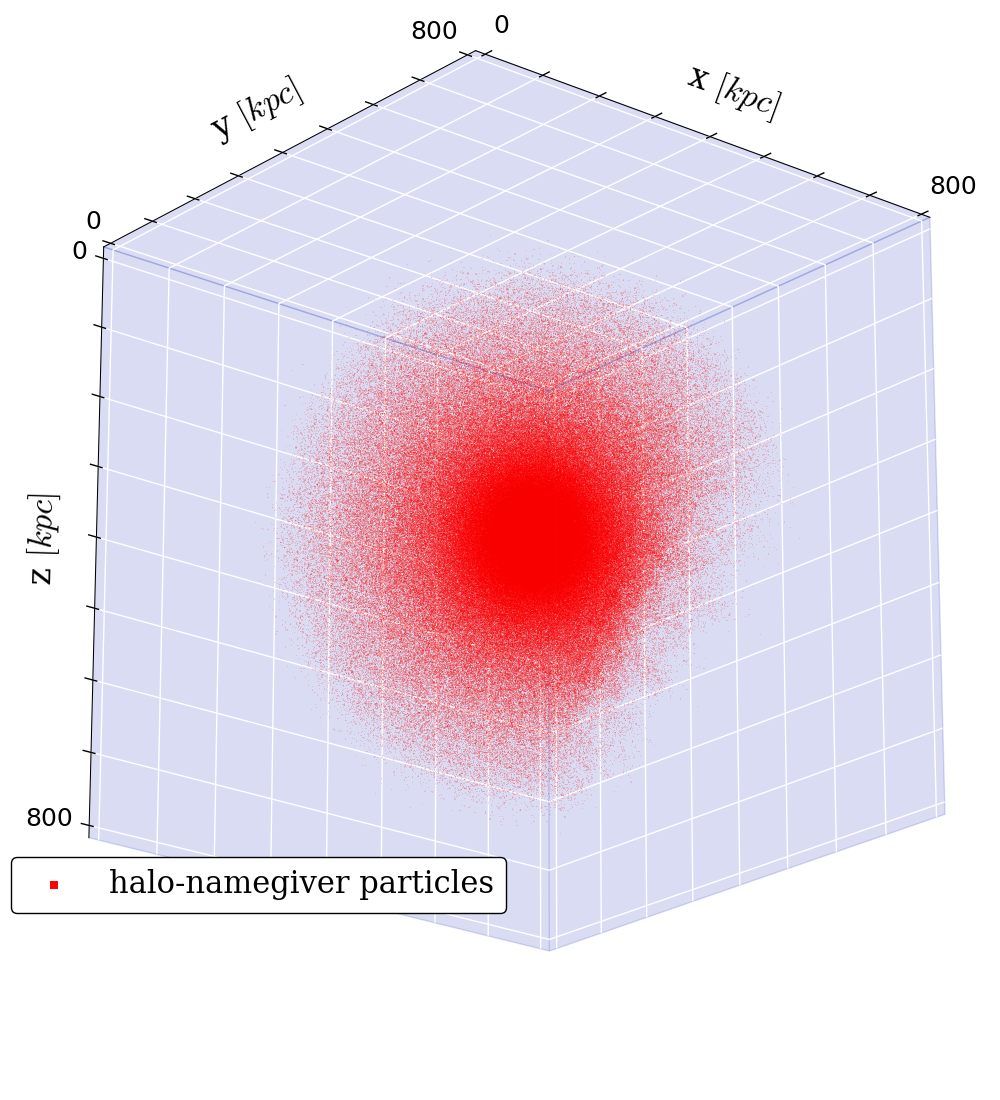
\includegraphics[width = .42\textwidth]{images/dice-sub/dice-sub-halo-only-phew.png}} \hspace*{-1em} 		&
				{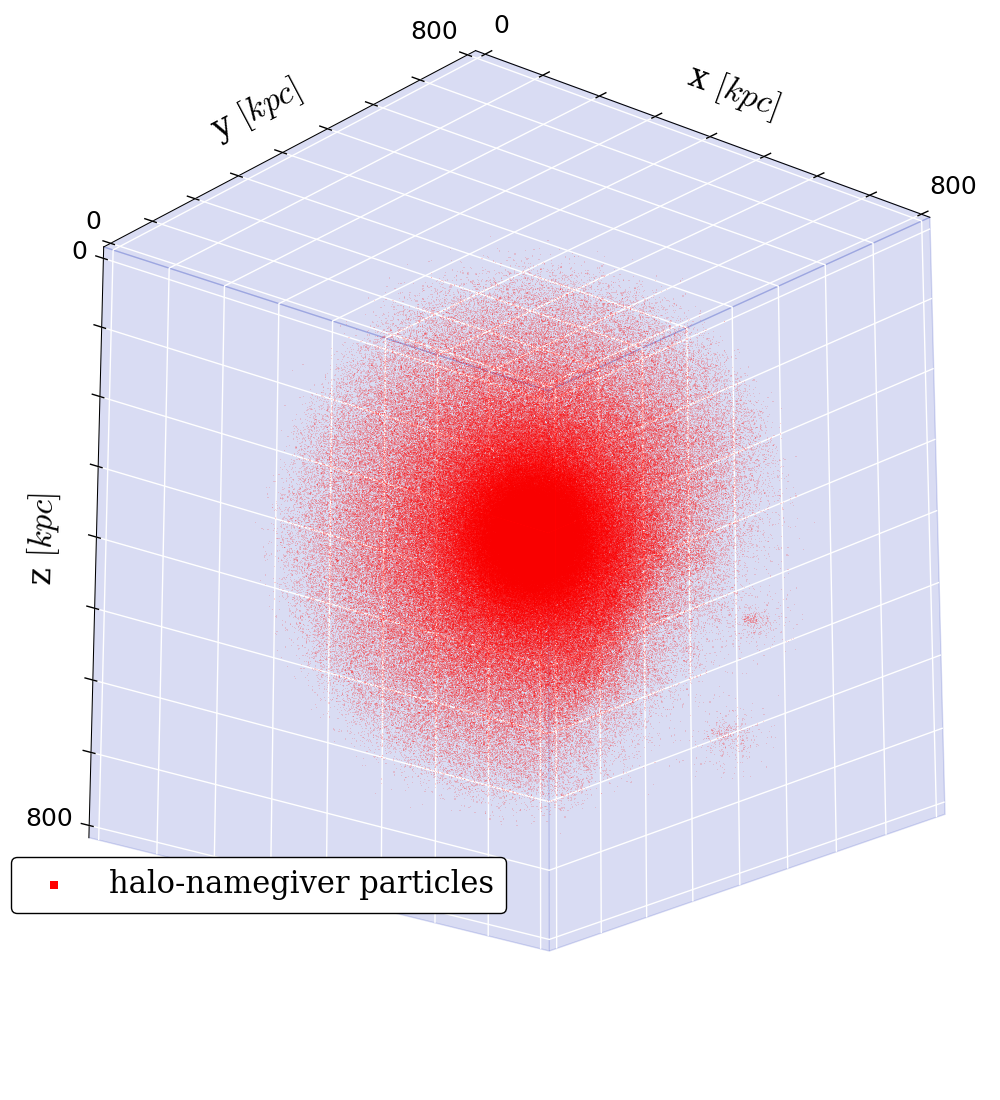
\includegraphics[width = .42\textwidth]{images/dice-sub/dice-sub-halo-only-nosaddle.png}} \hspace*{-1em}		\\
				%
				%
				\begin{sideways}{ \hspace{2cm}\textbf{Subhalo particles only} }\end{sideways}	 \hspace*{-1em}			 &
				{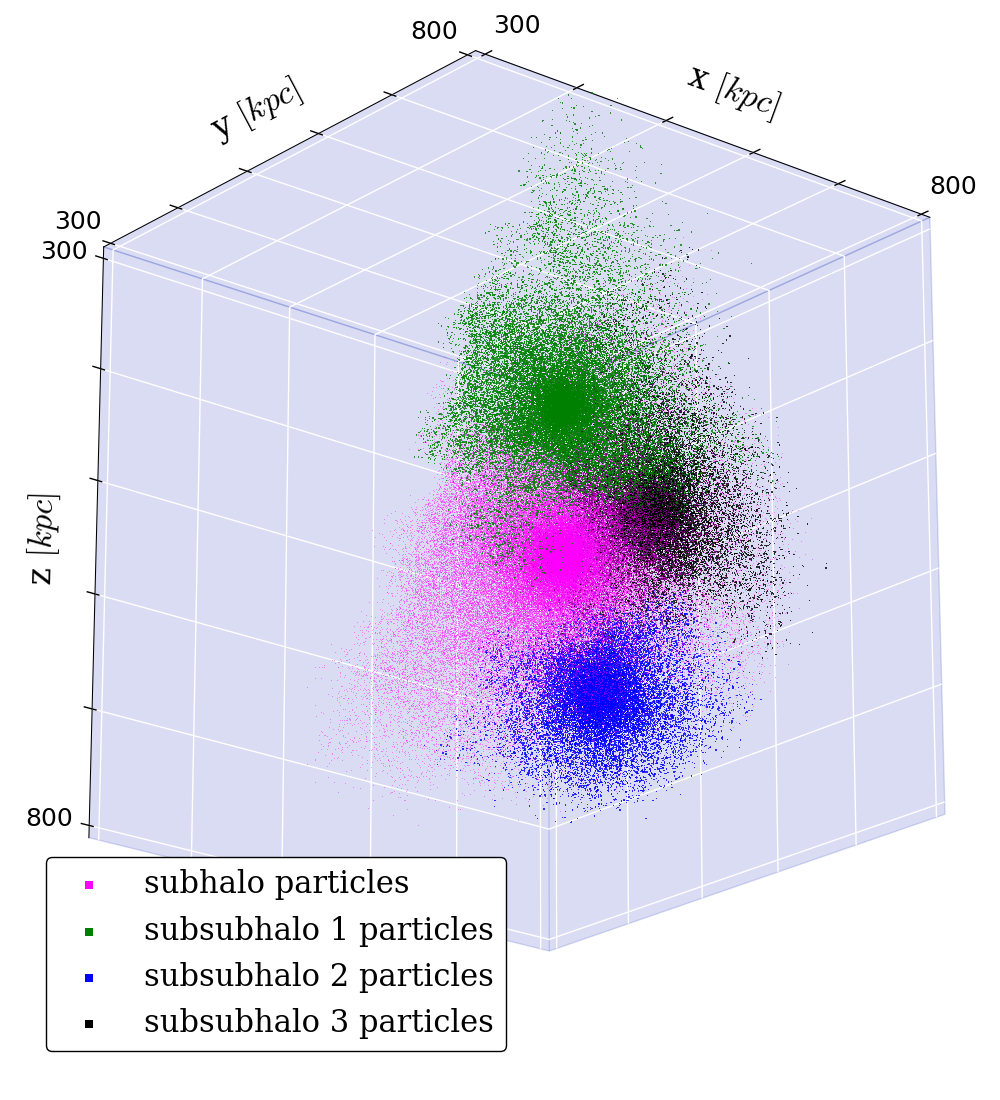
\includegraphics[width = .42\textwidth]{images/dice-sub/dice-sub-plot-subclumps-phew.png}} &
				{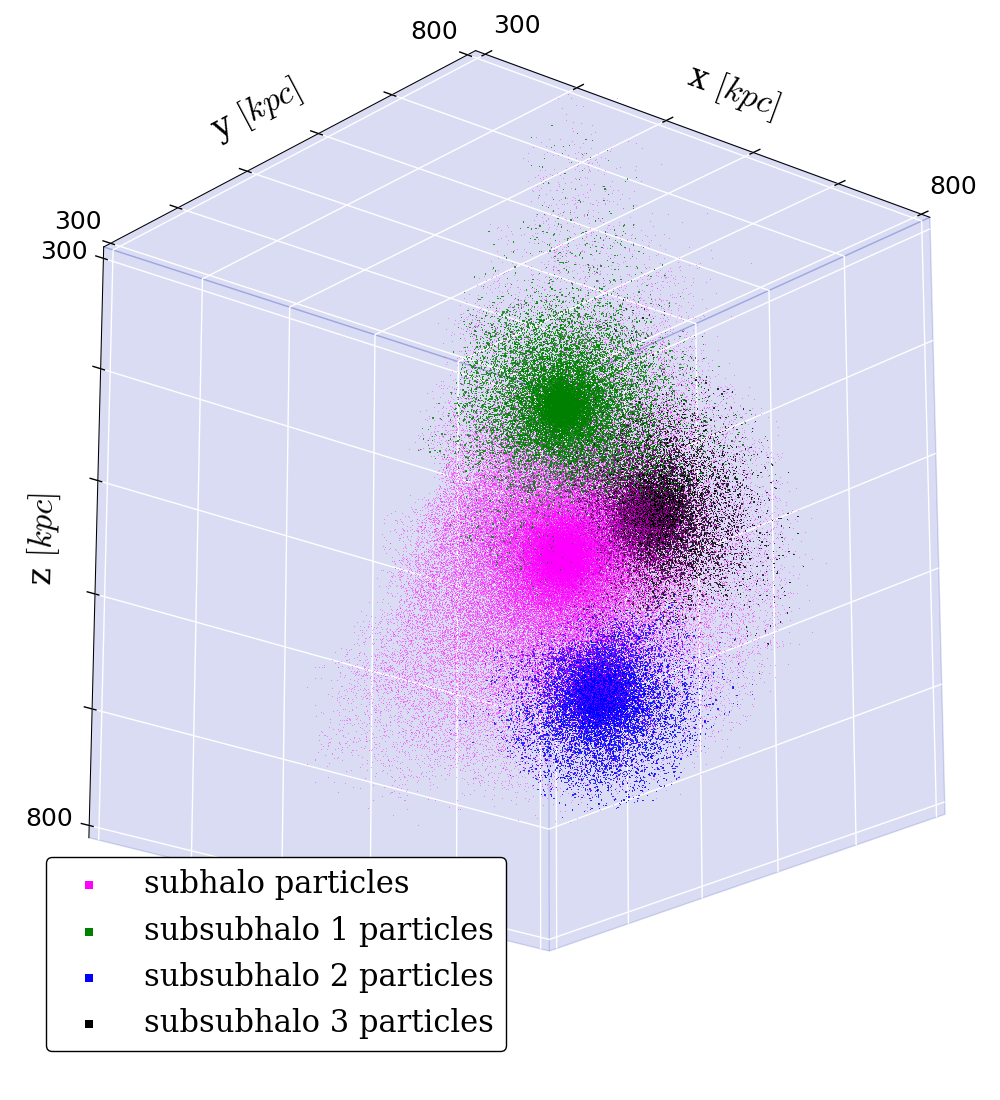
\includegraphics[width = .42\textwidth]{images/dice-sub/dice-sub-plot-subclumps-nosaddle.png}} \\
				\hline
			\end{tabular}
			\caption{\label{fig:dice_sub_results_a}The results of \phewon\ and \simple\ unbinding of the \ds-dataset: All particles, halo-namegiver particles only and subhalo particles only.}
		}
	\end{figure}
	%=================================================
	%=================================================
	%=================================================
	\begin{figure}[!htbp]%\ContinuedFloat
		{
			\renewcommand{\arraystretch}{0.1}
			\centering	
			\begin{tabular}{|p{.5cm} c c|}
				\hline
				&&\\[1em]
				&	\neigh\ 	& \iter \\[1.5em]
				%
				%
				\begin{sideways}{\hspace{3cm} \textbf{All particles}}\end{sideways} \hspace*{-1em}	&		 
				{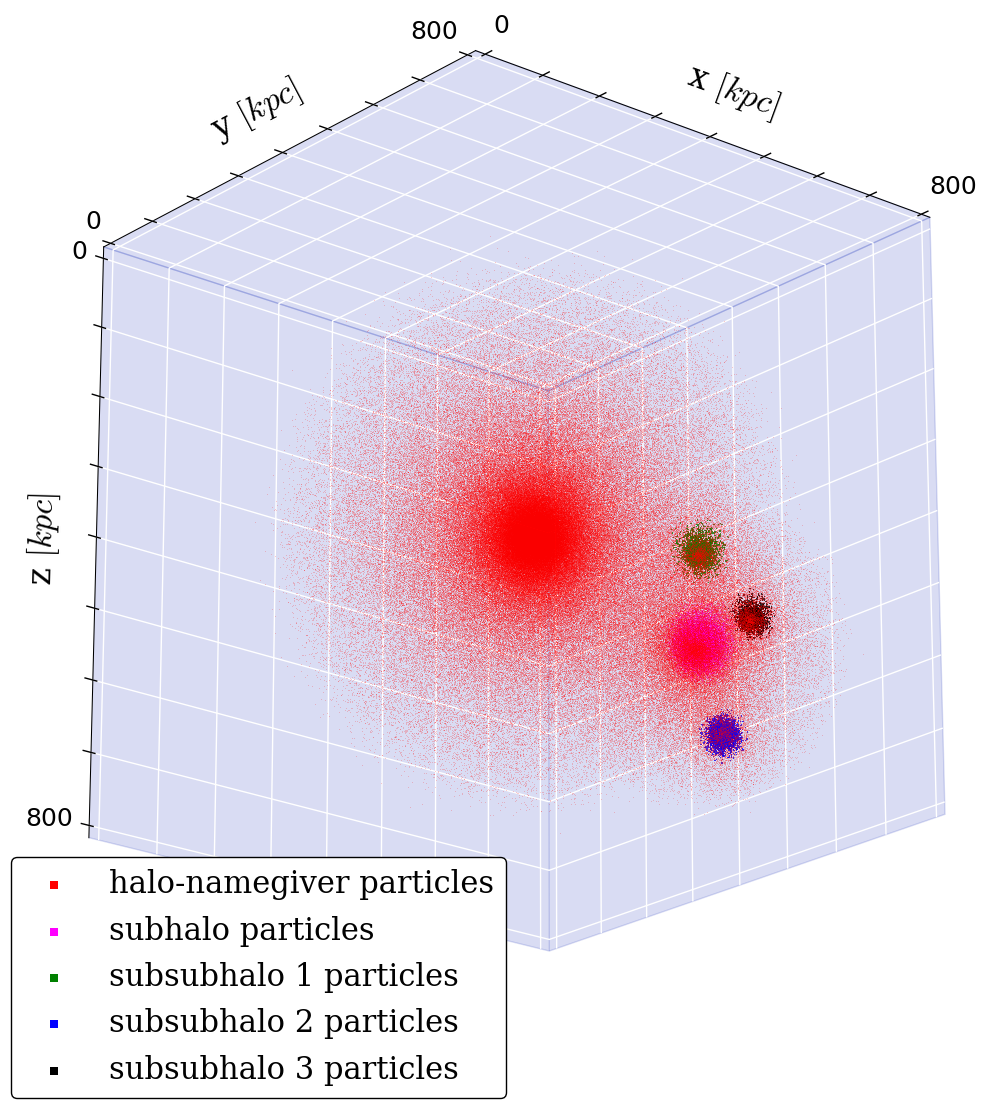
\includegraphics[width = .42\textwidth]{images/dice-sub/dice-sub-plot-halo1-saddle.png}} \hspace*{-1em} 	& 
				{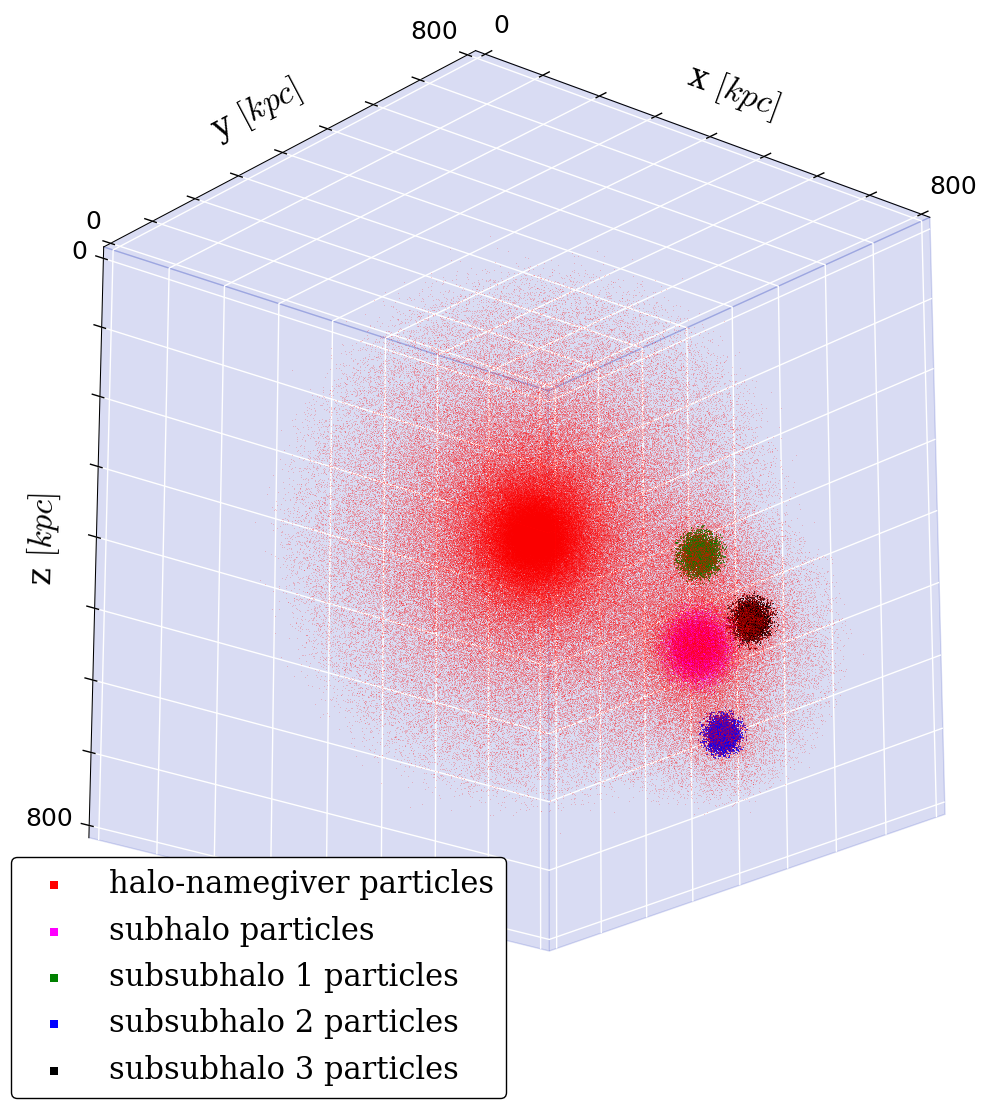
\includegraphics[width = .42\textwidth]{images/dice-sub/dice-sub-plot-halo1-iter.png}} \hspace*{-1em}	\\
				%
				%
				\begin{sideways}{ \hspace{.5cm}\textbf{Halo-namegiver particles only} }\end{sideways}	 \hspace*{-1em}			 &			 
				{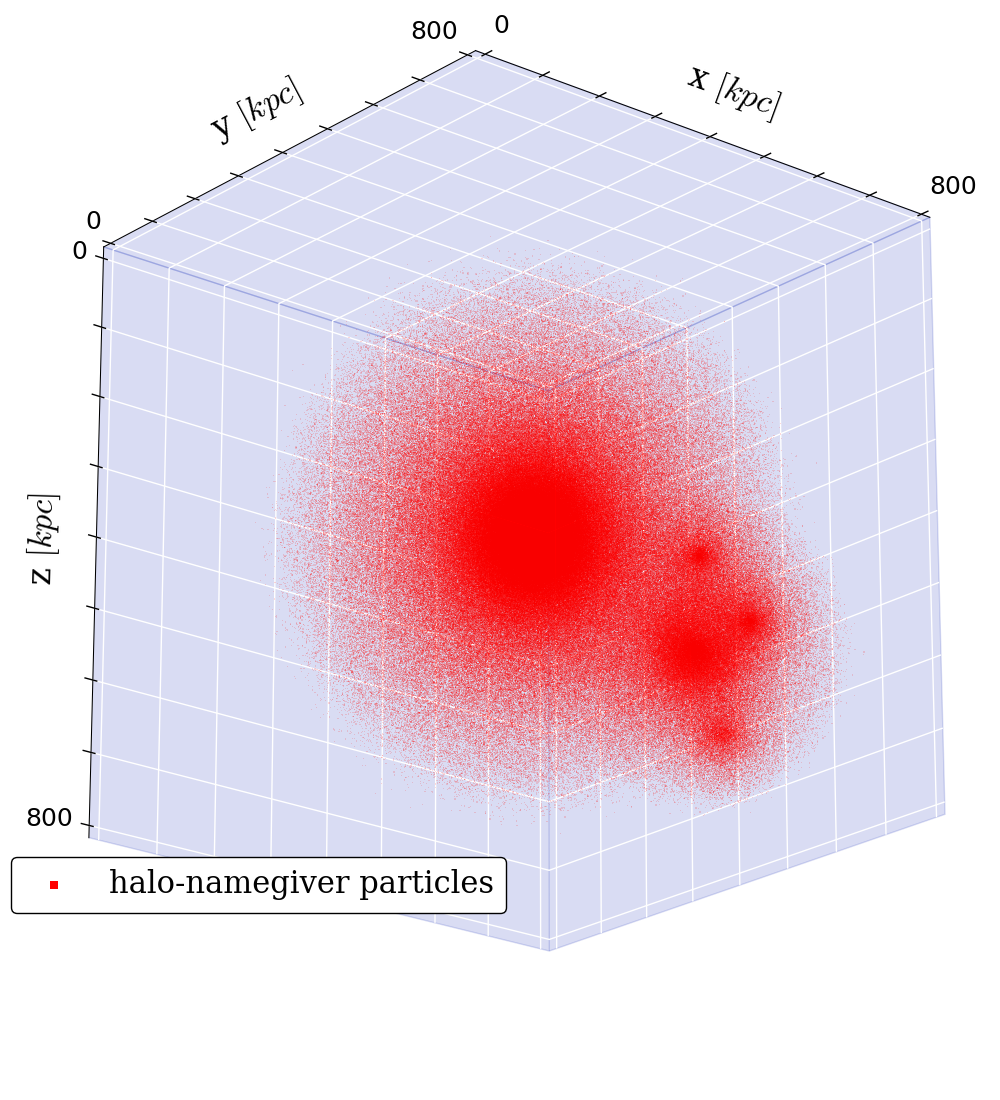
\includegraphics[width = .42\textwidth]{images/dice-sub/dice-sub-halo-only-saddle.png}} \hspace*{-1em} 		&
				{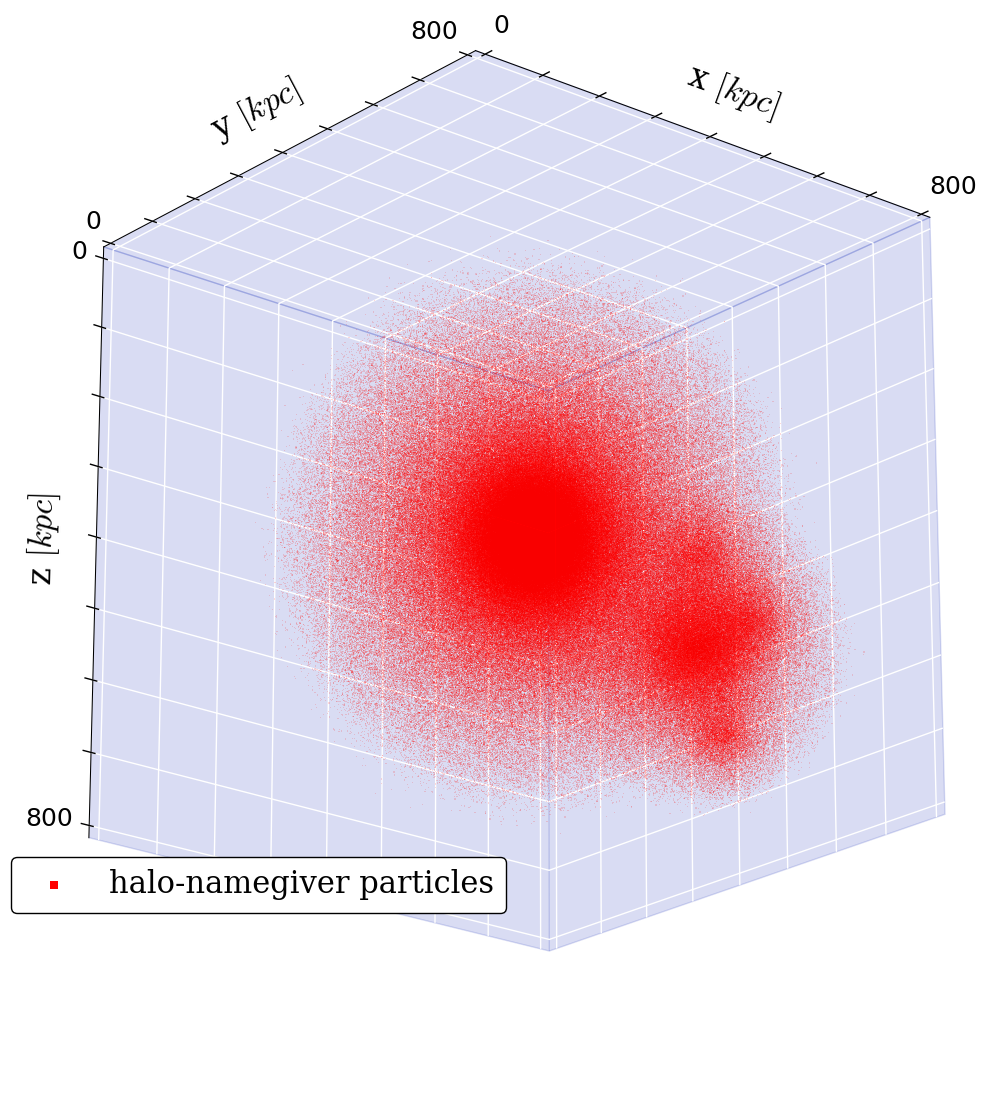
\includegraphics[width = .42\textwidth]{images/dice-sub/dice-sub-halo-only-iter.png}} \hspace*{-1em}		\\
				%
				%
				\begin{sideways}{ \hspace{2cm}\textbf{Subhalo particles only} }\end{sideways}	 \hspace*{-1em}			 &
				{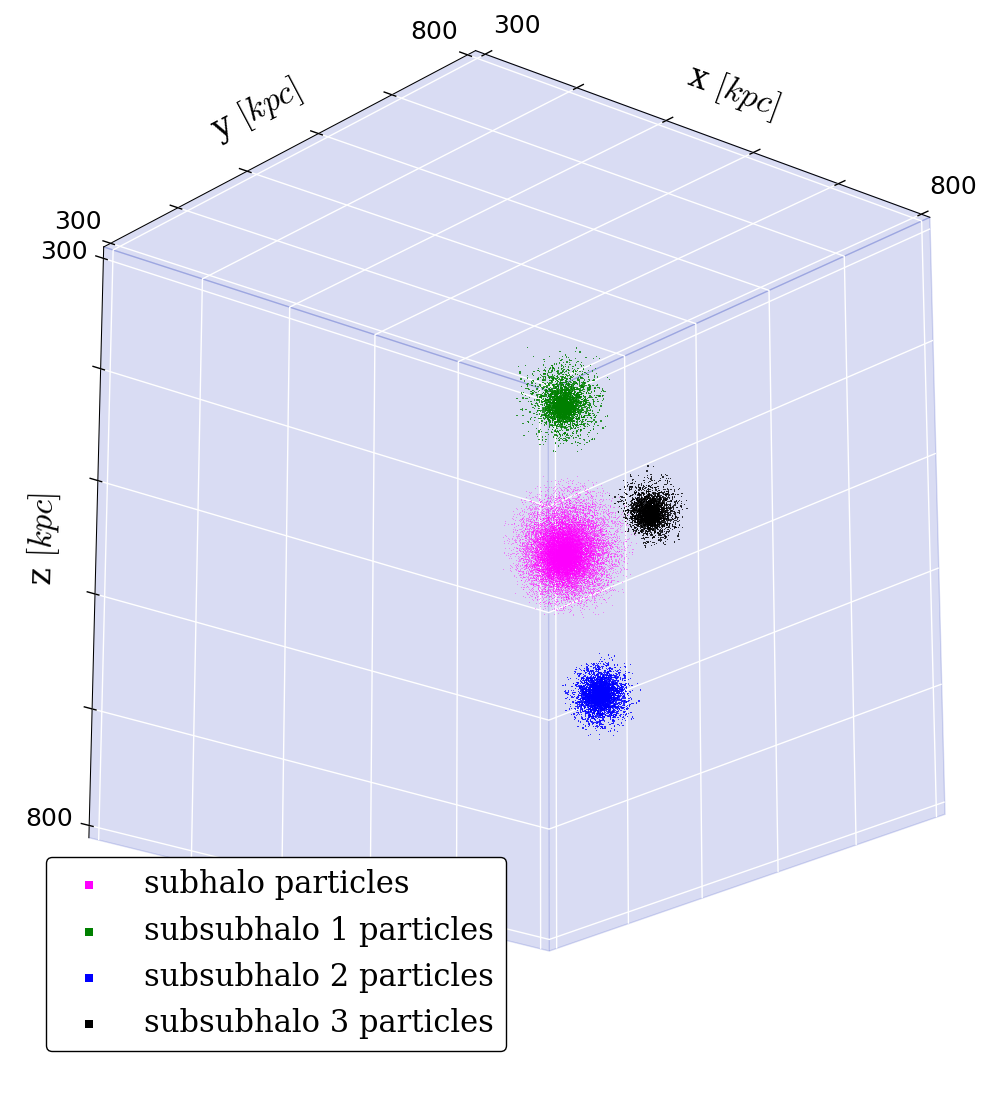
\includegraphics[width = .42\textwidth]{images/dice-sub/dice-sub-plot-subclumps-saddle.png}} &
				{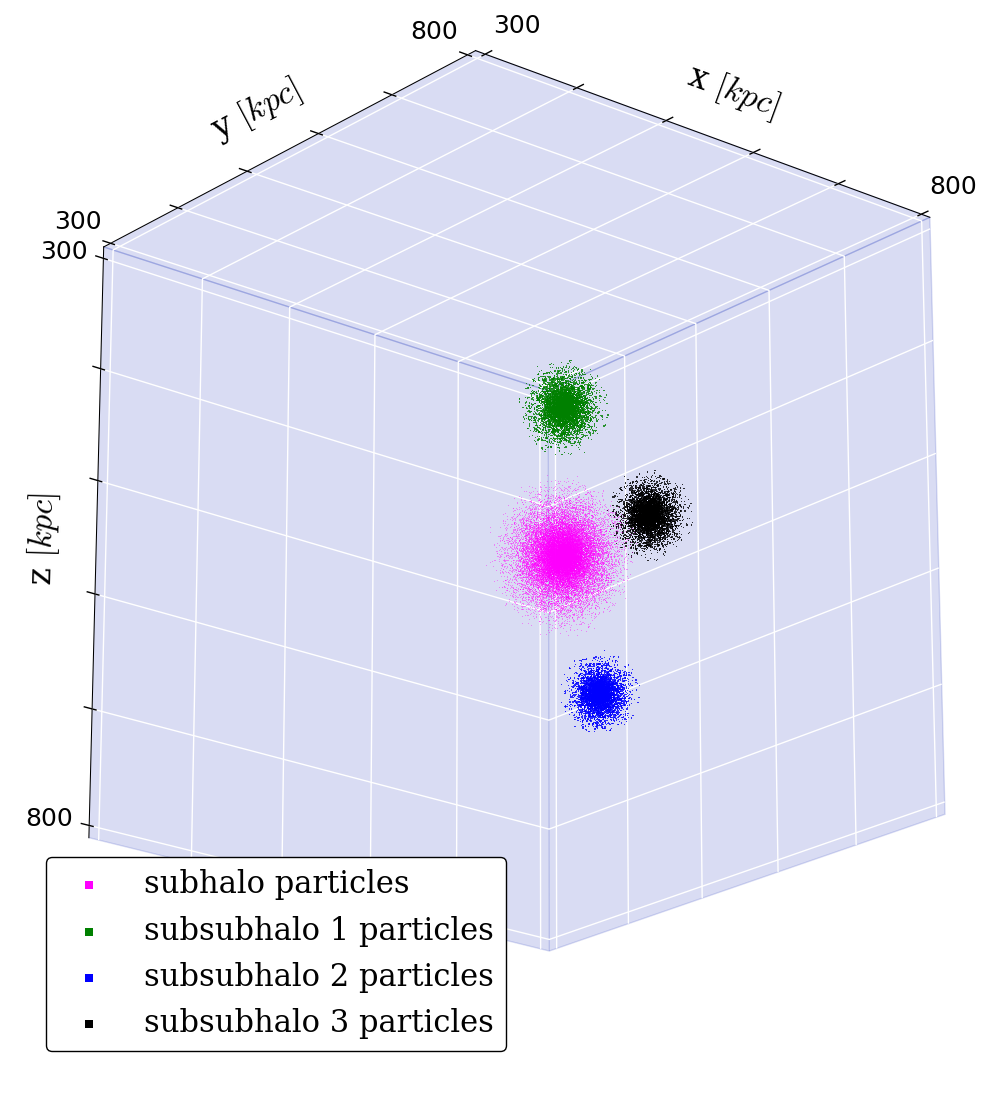
\includegraphics[width = .42\textwidth]{images/dice-sub/dice-sub-plot-subclumps-iter.png}} \\
				\hline
			\end{tabular}
			\caption{\label{fig:dice_sub_results_b}
				The results of \neigh\ and \iter\ unbinding of the \ds-dataset: All particles, halo-namegiver particles only and subhalo particles only.
			}
		}
	\end{figure}
	\label{fig:dice_sub_results}
\end{subfigures}




























































%\begin{sidewaysfigure}[!htbp]
%	{\renewcommand{\arraystretch}{0.1}
%		
%	\subfloat[The results of \phewon\ and \simple\ unbinding of the \ds-dataset: All particles, halo-namegiver particles only and subclumps particles only.]{
%		\begin{tabular}{|p{1cm} c c c|}
%			\hline
%			&&&\\[1em]
%													&
%			\textbf{All particles} 					&
%			\textbf{Halo-namegiver particles only} 	&
%			\textbf{Subhalo particles only} 		\\[1em]
%			%
%			%
%			\begin{sideways}{\hspace{3cm} \phewon}\end{sideways} \hspace*{-1em}%		 
%			& {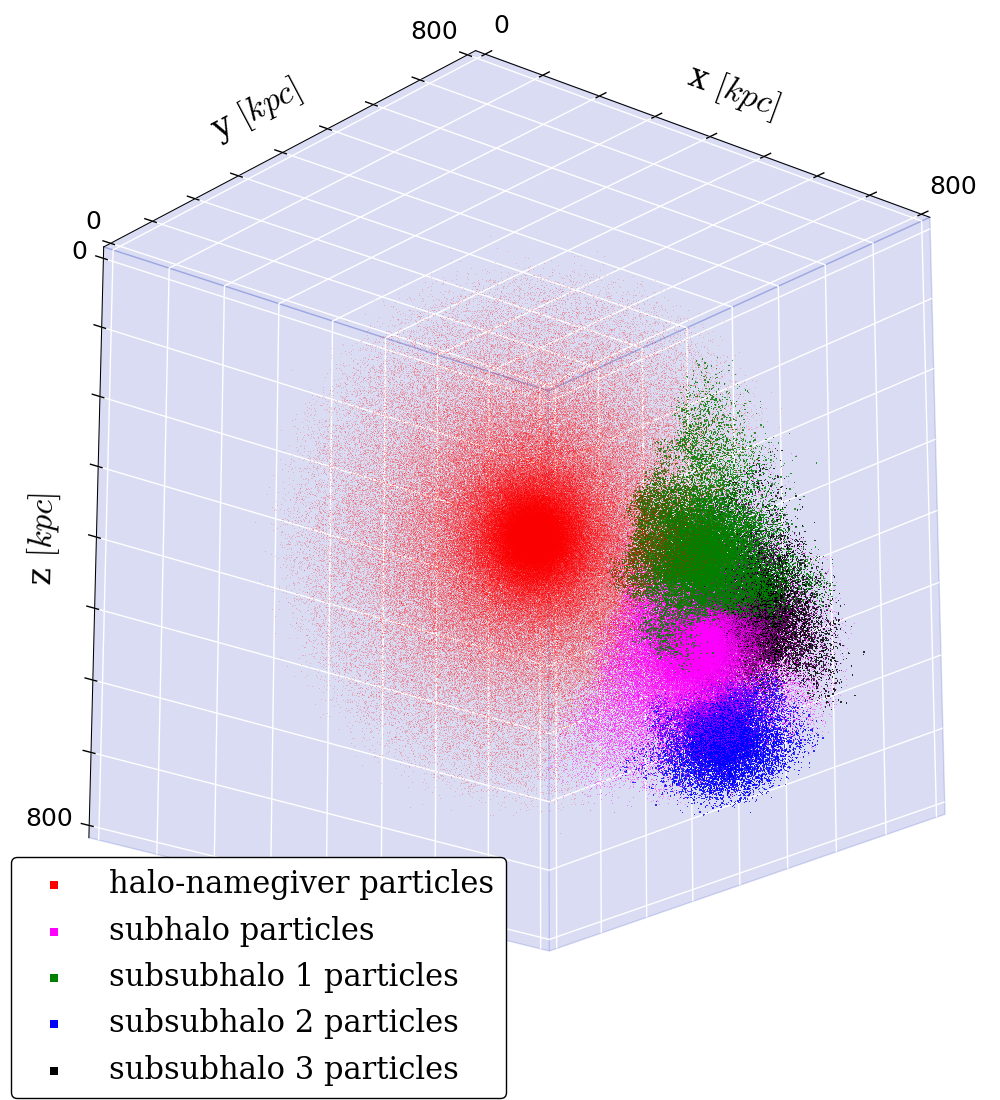
\includegraphics[width = .28\textwidth]{images/dice-sub/dice-sub-plot-halo1-phew.png}} \hspace*{-1em}%
%			 & {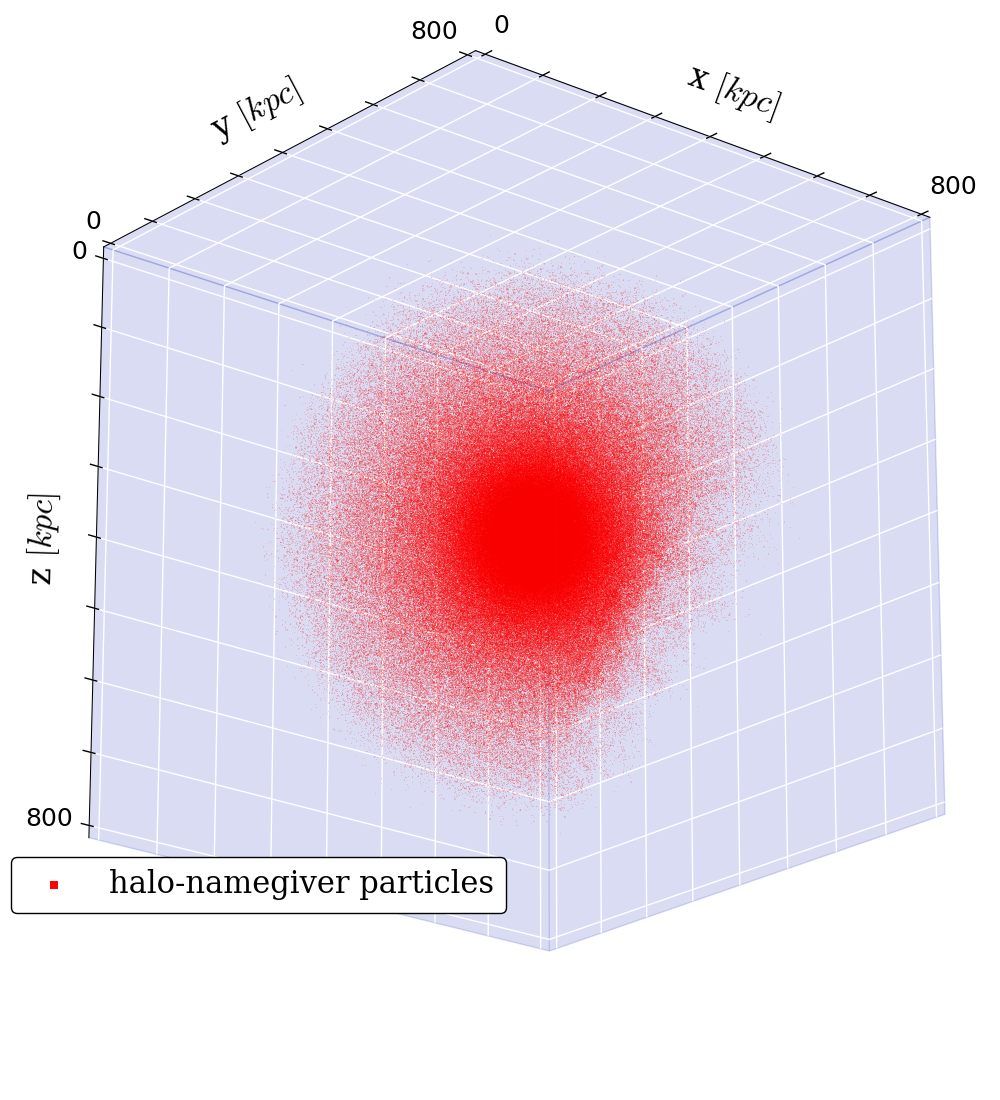
\includegraphics[width = .28\textwidth]{images/dice-sub/dice-sub-halo-only-phew.png}} \hspace*{-1em}% 
%			 &{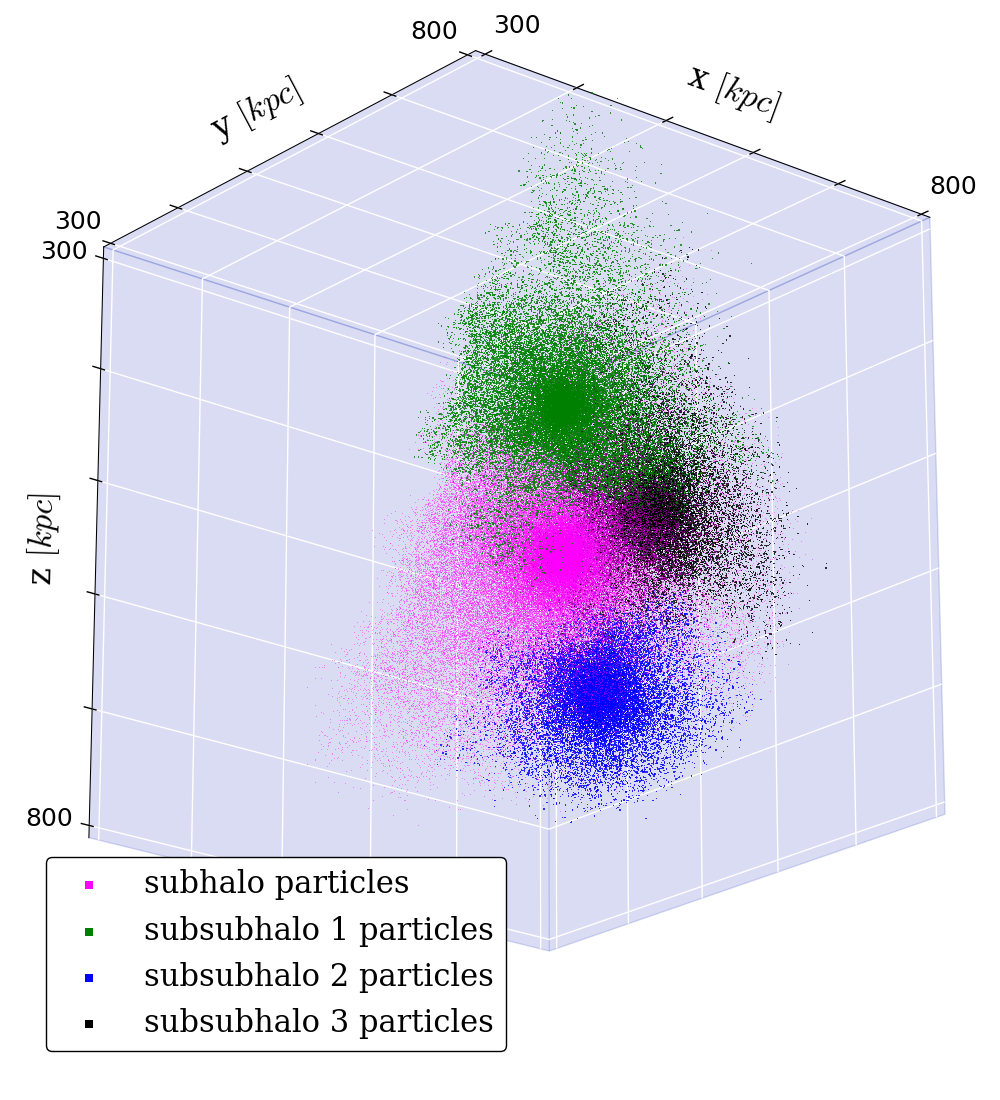
\includegraphics[width = .28\textwidth]{images/dice-sub/dice-sub-plot-subclumps-phew.png}} \\
%			%
%			%
%			\begin{sideways}{ \hspace{3cm}\simple\ unbinding }\end{sideways}	 \hspace*{-1em}			 &
%			{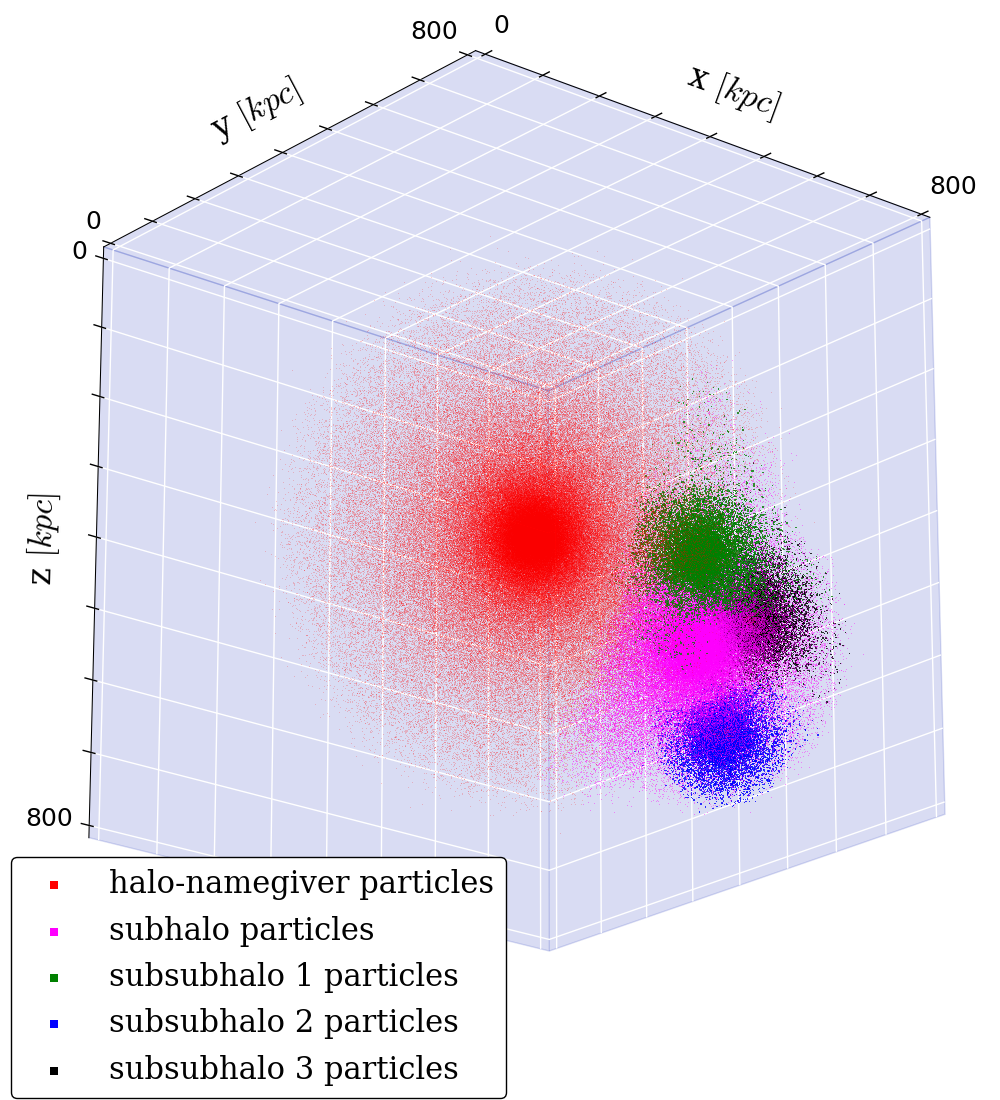
\includegraphics[width = .28\textwidth]{images/dice-sub/dice-sub-plot-halo1-nosaddle.png}} \hspace*{-1em}&
%			{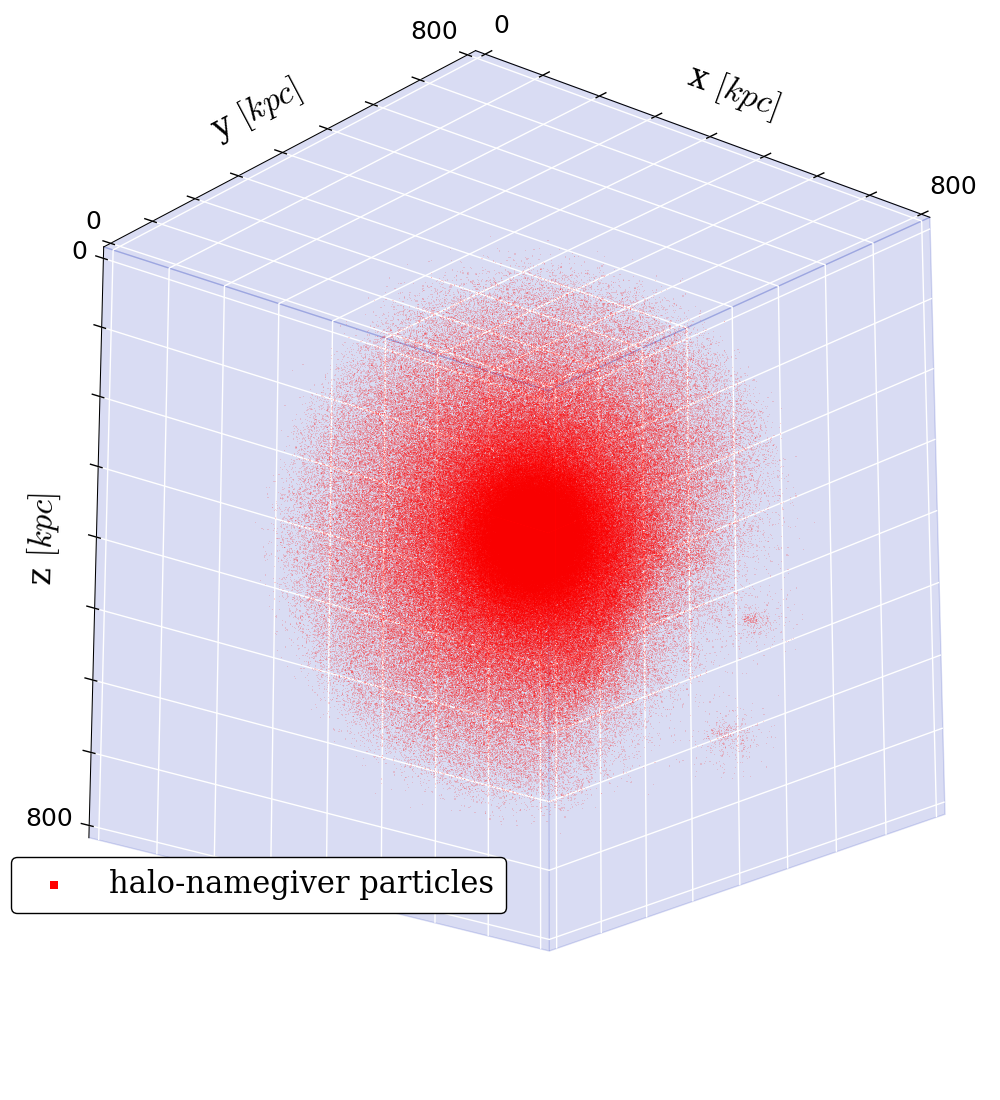
\includegraphics[width = .28\textwidth]{images/dice-sub/dice-sub-halo-only-nosaddle.png}} \hspace*{-1em}&
%			{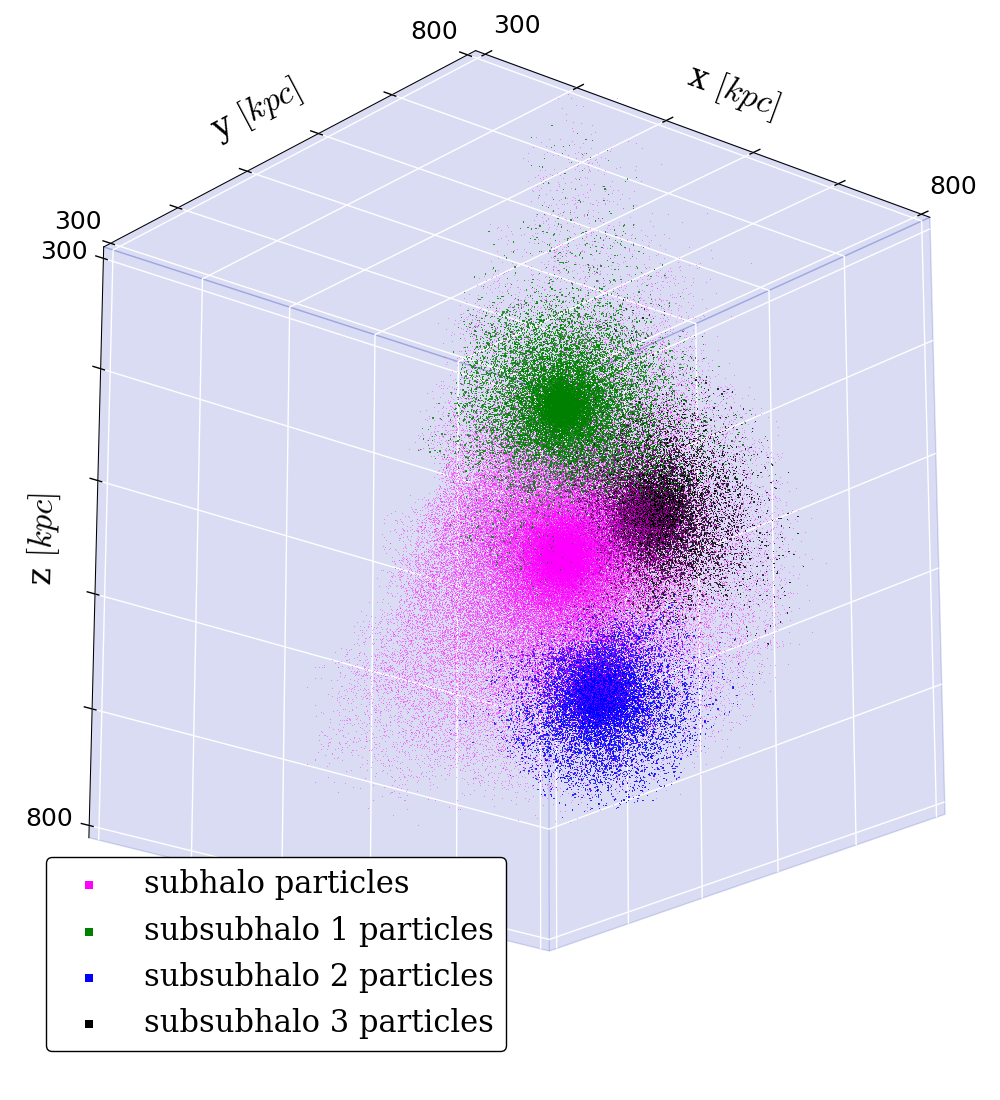
\includegraphics[width = .28\textwidth]{images/dice-sub/dice-sub-plot-subclumps-nosaddle.png}} \\
%			\hline
%		\end{tabular}
%		\label{fig:dice_sub_results_a}
%		}
%	}
%	\phantomcaption
%\end{sidewaysfigure}
%%=================================================
%%=================================================
%%=================================================
%\begin{sidewaysfigure}[!htbp]\ContinuedFloat
%	\footnotesize
%	{\renewcommand{\arraystretch}{0.1}
%	\subfloat[The results of \neigh\ and \iter\ unbinding of the \ds-dataset: All particles, halo-namegiver particles only and subclumps particles only.]{
%		\begin{tabular}{|p{1cm} c c c|}
%			\hline
%			&&&\\[1em]
%													&
%			\textbf{All particles} 					&
%			\textbf{Halo-namegiver particles only} 	&
%			\textbf{Subhalo particles only}			\\[1em]
%			%
%			%
%			\begin{sideways}{ \hspace{3cm}\neigh\ unbinding }\end{sideways}		\hspace*{-1em}		 &		
%			{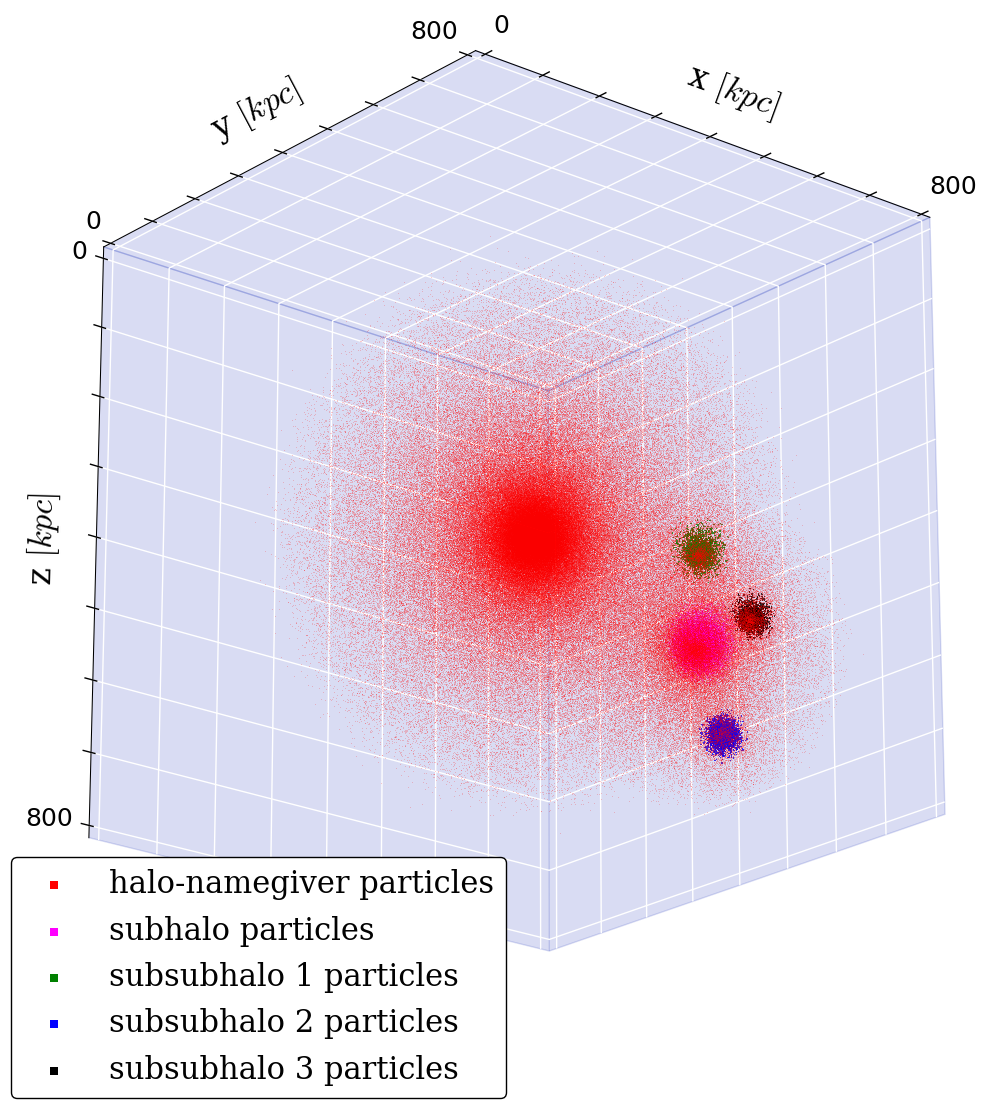
\includegraphics[width = .28\textwidth]{images/dice-sub/dice-sub-plot-halo1-saddle.png}}\hspace*{-1em} &
%			{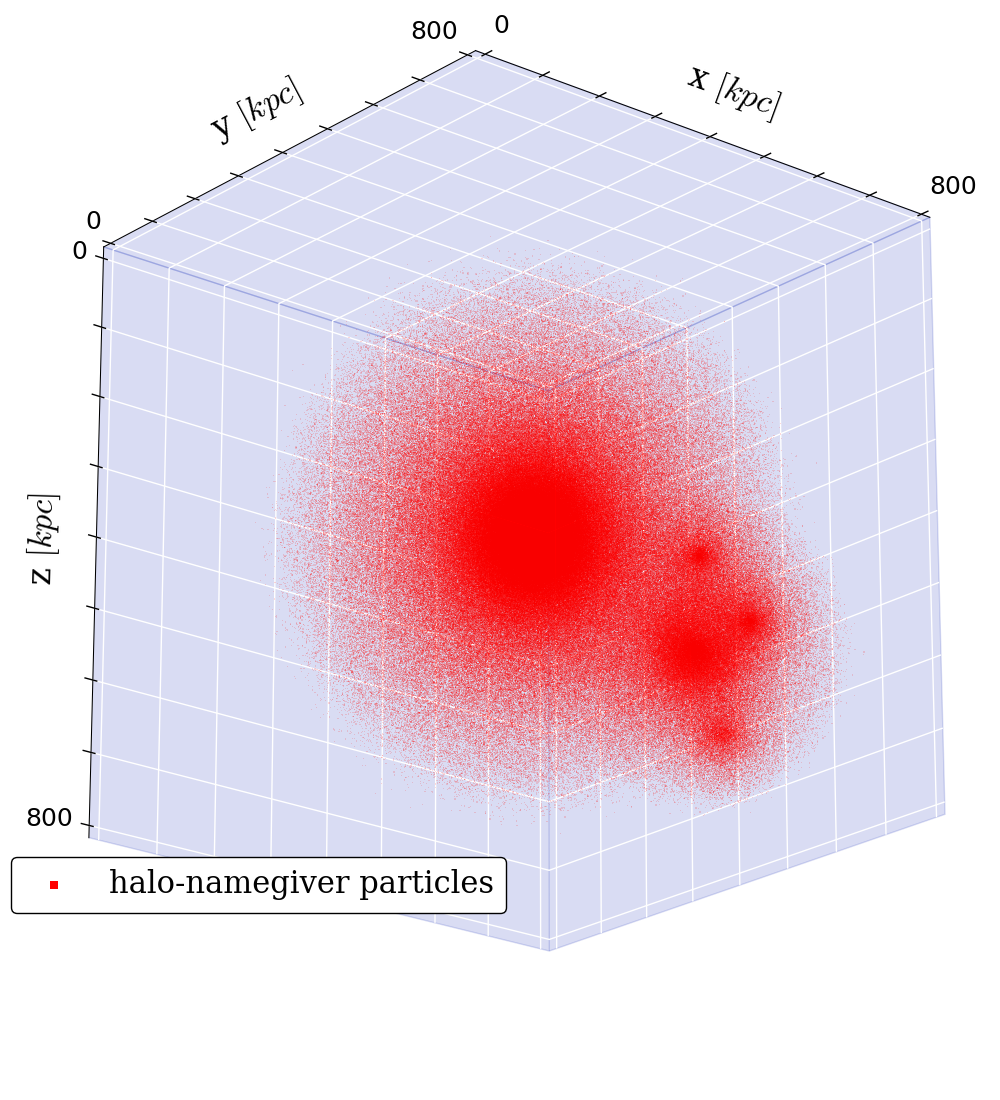
\includegraphics[width = .28\textwidth]{images/dice-sub/dice-sub-halo-only-saddle.png}}\hspace*{-1em} &
%			{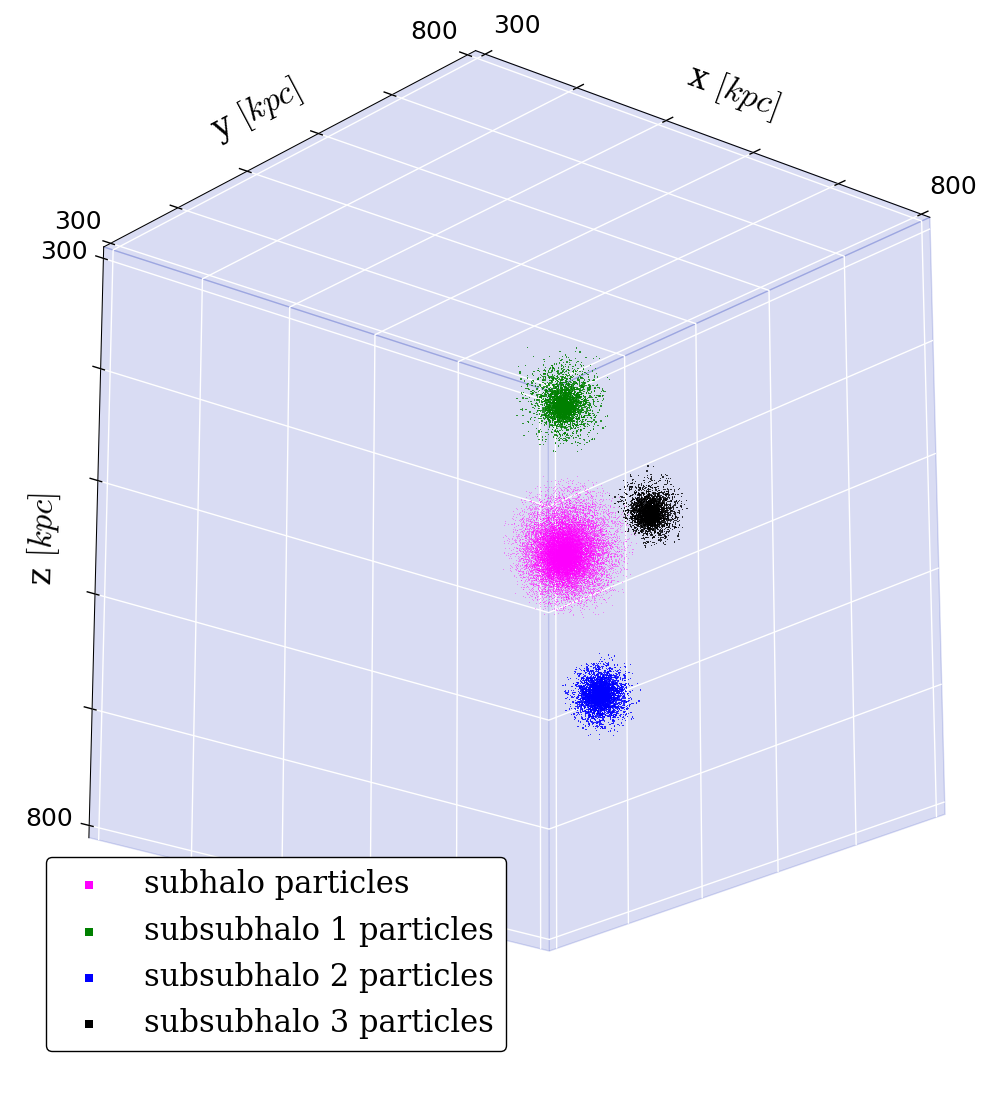
\includegraphics[width = .28\textwidth]{images/dice-sub/dice-sub-plot-subclumps-saddle.png}} \\
%	%		%
%	%		%
%			\begin{sideways}{\hspace{3cm} \iter\ unbinding }\end{sideways}		\hspace*{-1em}		 &		
%			{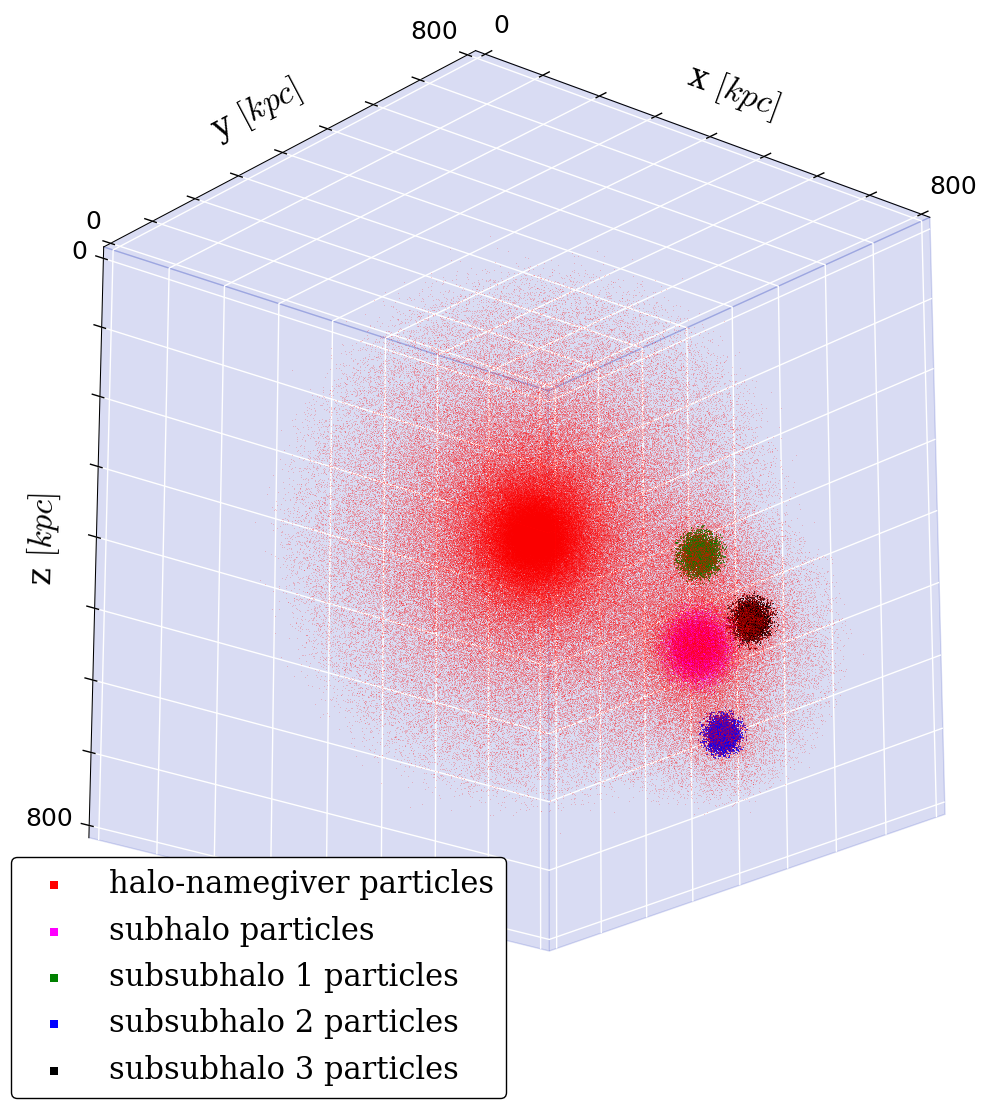
\includegraphics[width = .28\textwidth]{images/dice-sub/dice-sub-plot-halo1-iter.png}} \hspace*{-1em}&
%			{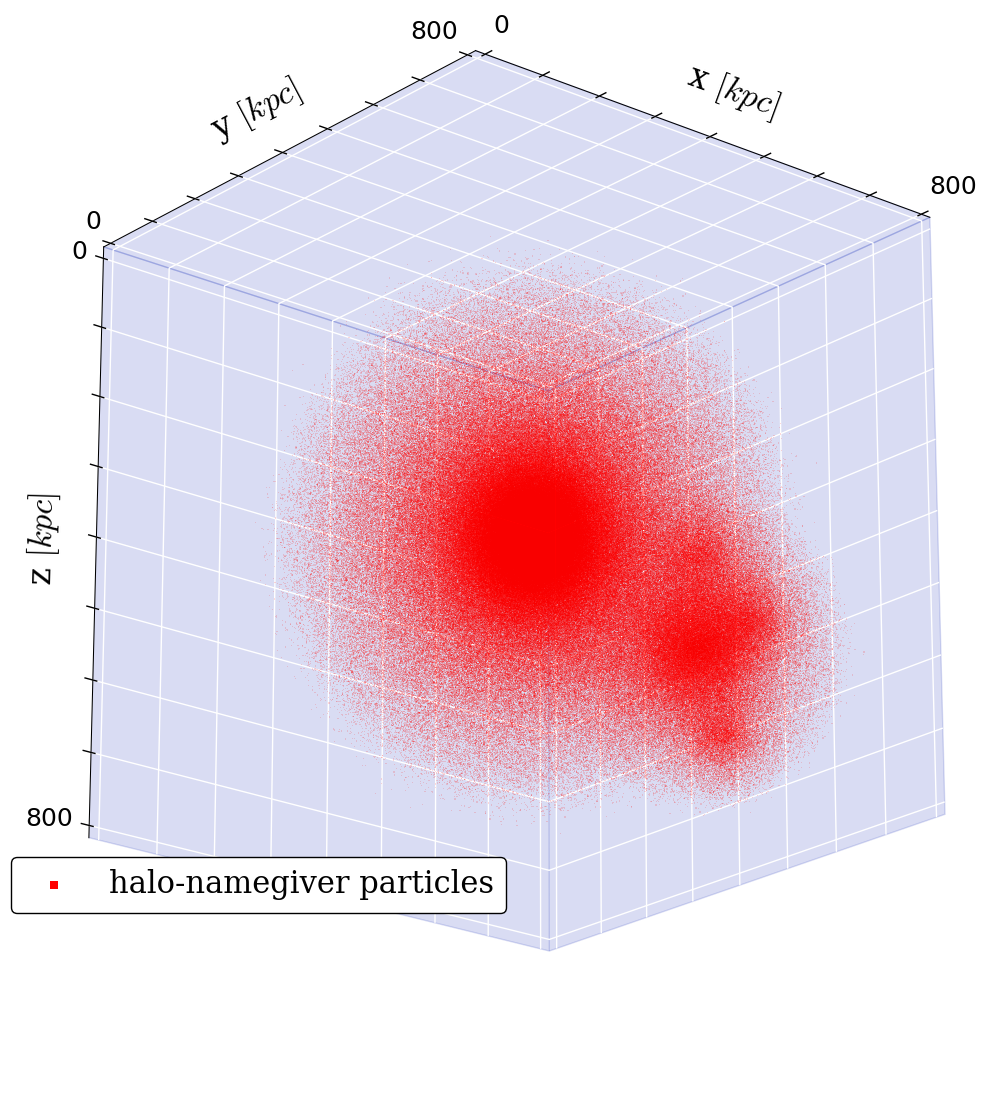
\includegraphics[width = .28\textwidth]{images/dice-sub/dice-sub-halo-only-iter.png}} \hspace*{-1em}&
%			{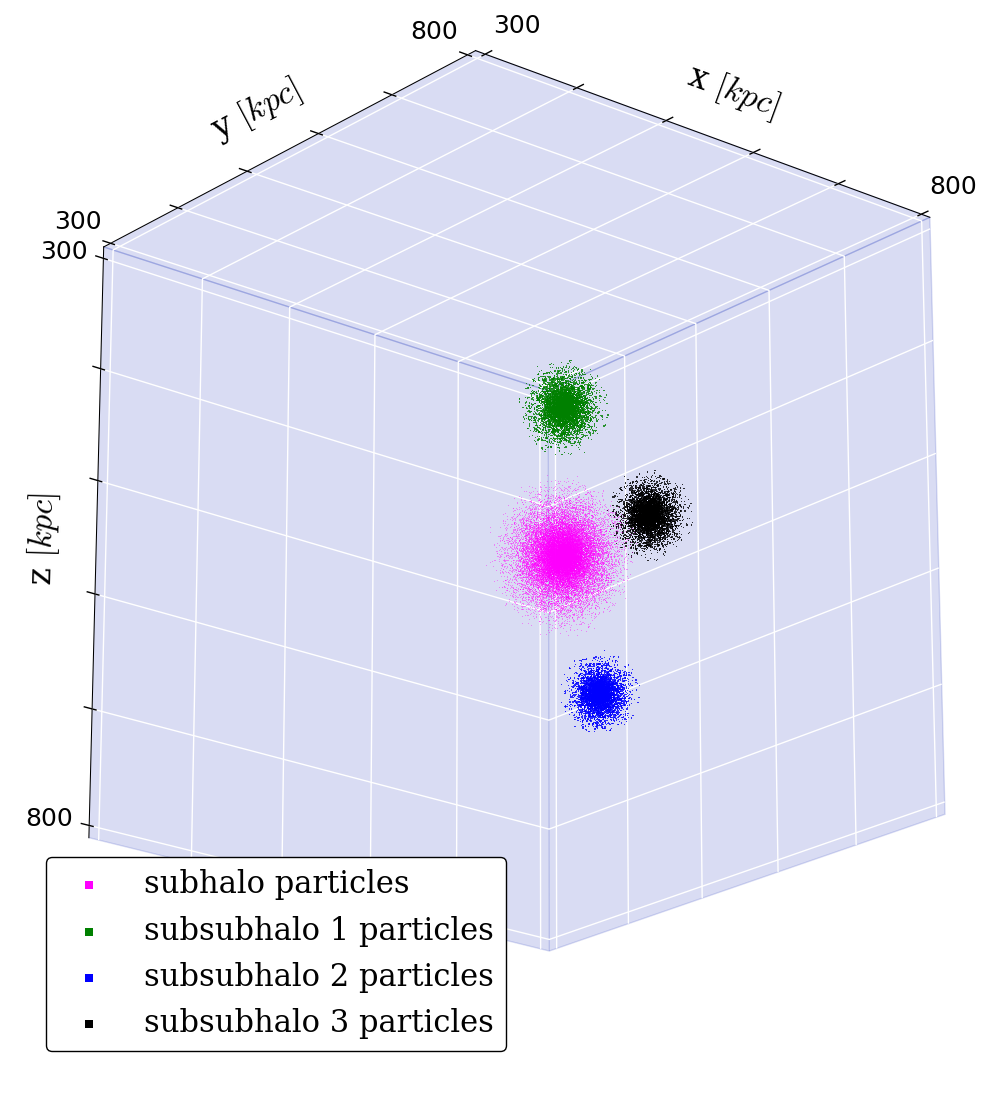
\includegraphics[width = .28\textwidth]{images/dice-sub/dice-sub-plot-subclumps-iter.png}} \\
%			%
%			%
%			\hline
%		\end{tabular}
%		\label{fig:dice_sub_results_b}
%		}
%	}
%	\caption{
%	The results of different unbinding methods on the \dt-dataset.
%	}
%	\label{fig:dice_sub_results}
%\end{sidewaysfigure}
%
%







%=====================
% Cosmo
%=====================

\begin{subfigures}
	\begin{figure}[!htbp]
		{
			\renewcommand{\arraystretch}{0.1}		
			\centering	
			%	\subfloat[]{
			\begin{tabular}{|p{.5cm} c c|}
				\hline
				&&\\[1em]
				&	\phewon\ 	& \simple \\[1.5em]
				%
				%
				\begin{sideways}{\hspace{3cm} \textbf{All particles}}\end{sideways} \hspace*{-1em}	&		 
				{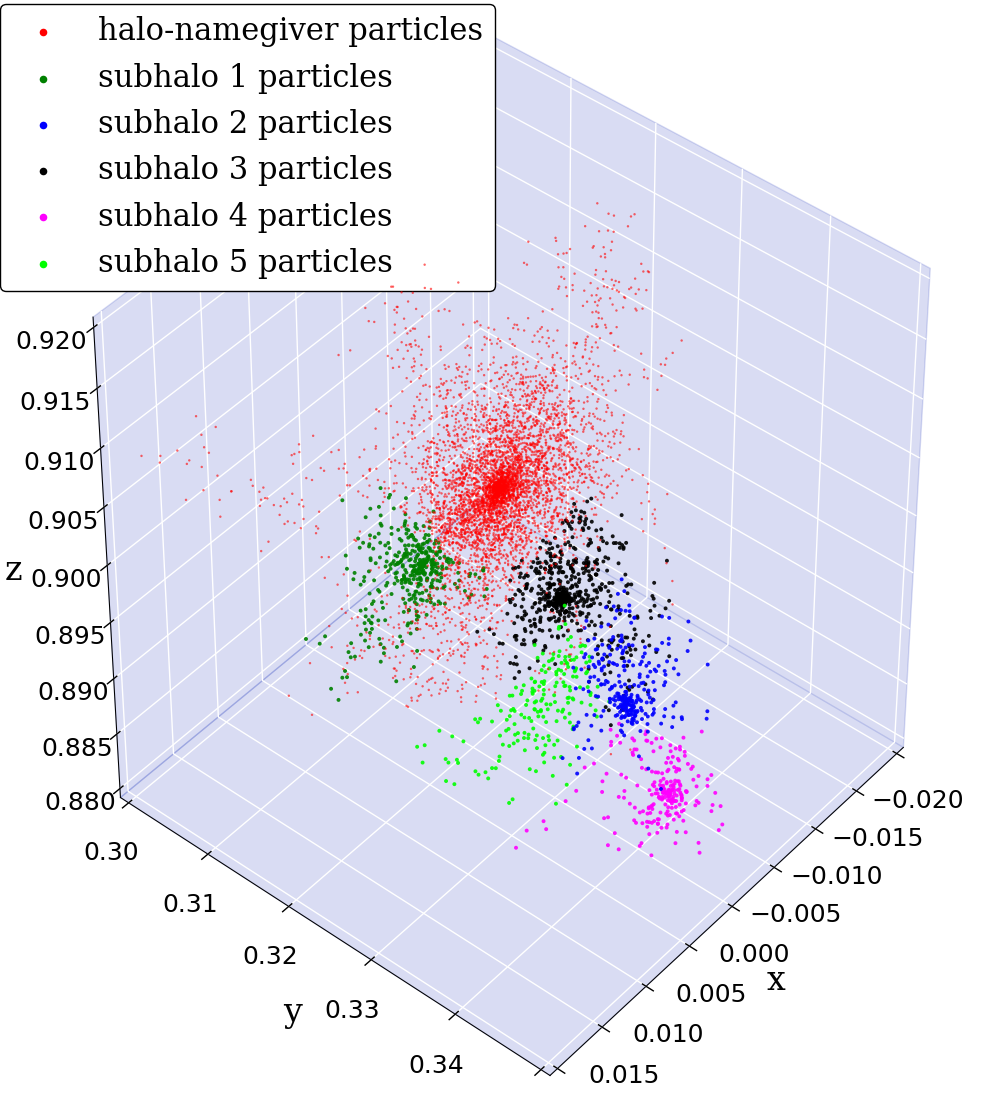
\includegraphics[width = .42\textwidth]{images/cosmo/cos-halo-66858-phew.png}} \hspace*{-1em} 	& 
				{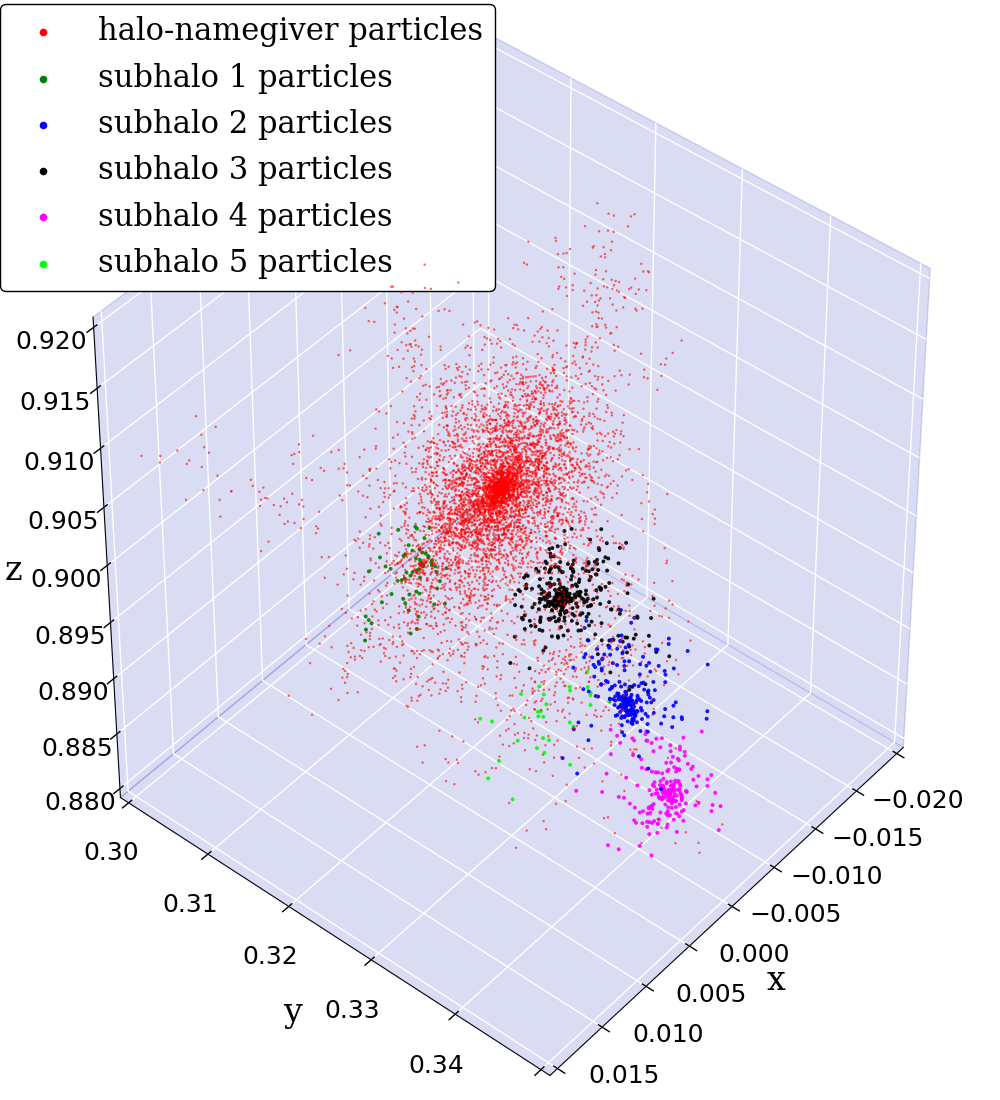
\includegraphics[width = .42\textwidth]{images/cosmo/cos-halo-66858-nosaddle.png}} \hspace*{-1em}	\\
				%
				%
				\begin{sideways}{ \hspace{.5cm}\textbf{Halo-namegiver particles only} }\end{sideways}	 \hspace*{-1em}			 &			 
				{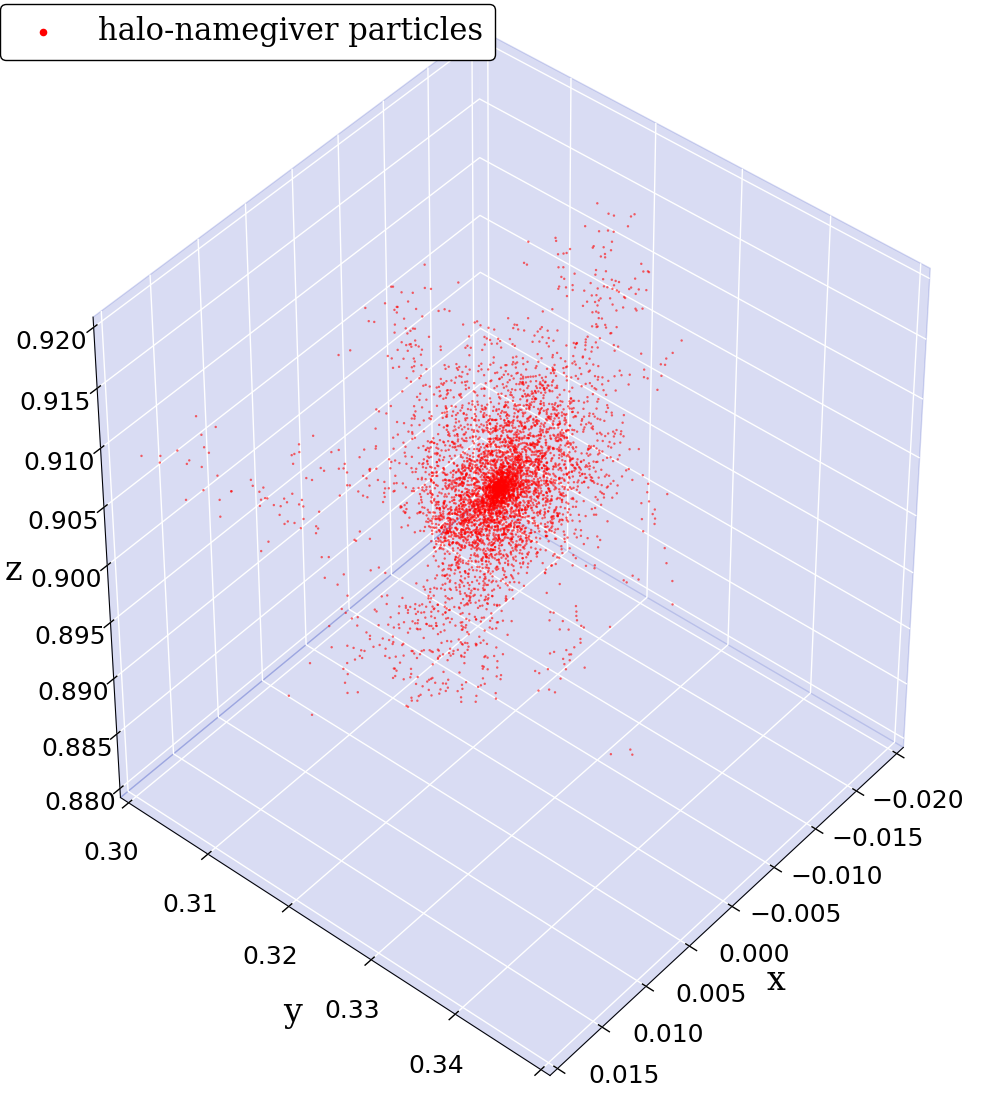
\includegraphics[width = .42\textwidth]{images/cosmo/cos-halo-66858-halo-only-phew.png}} \hspace*{-1em} 		&
				{\includegraphics[width = .42\textwidth]{images/cosmo/cos-halo-66858-halo-only-nosaddle.png}} \hspace*{-1em}		\\
				%
				%
				\begin{sideways}{ \hspace{2cm}\textbf{Subhalo particles only} }\end{sideways}	 \hspace*{-1em}			 &
				{\includegraphics[width = .42\textwidth]{images/cosmo/cos-halo-66858-subhalo-only-phew.png}} &
				{\includegraphics[width = .42\textwidth]{images/cosmo/cos-halo-66858-subhalo-only-nosaddle.png}} \\
				\hline
			\end{tabular}
			\caption{\label{fig:cosmo_results_a}The results of \phewon\ and \simple\ unbinding of the \cosmo-dataset: All particles, halo-namegiver particles only and subhalo particles only.}
		}
	\end{figure}
	%=================================================
	%=================================================
	%=================================================
	\begin{figure}[!htbp]%\ContinuedFloat
		{
			\renewcommand{\arraystretch}{0.1}
			\centering	
			\begin{tabular}{|p{.5cm} c c|}
				\hline
				&&\\[1em]
				&	\neigh\ 	& \iter \\[1.5em]
				%
				%
				\begin{sideways}{\hspace{3cm} \textbf{All particles}}\end{sideways} \hspace*{-1em}	&		 
				{\includegraphics[width = .42\textwidth]{images/cosmo/cos-halo-66858-saddle.png}} \hspace*{-1em} 	& 
				{\includegraphics[width = .42\textwidth]{images/cosmo/cos-halo-66858-iter.png}} \hspace*{-1em}	\\
				%
				%
				\begin{sideways}{ \hspace{.5cm}\textbf{Halo-namegiver particles only} }\end{sideways}	 \hspace*{-1em}			 &			 
				{\includegraphics[width = .42\textwidth]{images/cosmo/cos-halo-66858-halo-only-saddle.png}} \hspace*{-1em} 		&
				{\includegraphics[width = .42\textwidth]{images/cosmo/cos-halo-66858-halo-only-iter.png}} \hspace*{-1em}		\\
				%
				%
				\begin{sideways}{ \hspace{2cm}\textbf{Subhalo particles only} }\end{sideways}	 \hspace*{-1em}			 &
				{\includegraphics[width = .42\textwidth]{images/cosmo/cos-halo-66858-subhalo-only-saddle.png}} &
				{\includegraphics[width = .42\textwidth]{images/cosmo/cos-halo-66858-subhalo-only-iter.png}} \\
				\hline
			\end{tabular}
			\caption{\label{fig:cosmo_results_b}
				The results of \neigh\ and \iter\ unbinding of the \cosmo-dataset: All particles, halo-namegiver particles only and subhalo particles only.
			}
		}
	\end{figure}
	\label{fig:cosmo_results}
\end{subfigures}






































%
%
%\begin{sidewaysfigure}[!htbp]
%	{\renewcommand{\arraystretch}{0.1}
%		
%	\subfloat[The results of \phewon\ and \simple\ unbinding of the \cosmo-dataset: All particles, halo-namegiver particles only and subhalo particles only.]{
%		\begin{tabular}{|p{1cm} c c c|}
%			\hline
%			&&&\\[1em]
%													&
%			\textbf{All particles} 					&
%			\textbf{Halo-namegiver particles only} 	&
%			\textbf{Subhalo particles only} 		\\[1em]
%			%
%			%
%			\begin{sideways}{\hspace{3cm} \phewon}\end{sideways} \hspace*{-1em}%		 
%			& {\includegraphics[width = .42\textwidth]{images/cosmo/cos-halo-66858-phew.png}} \hspace*{-1em}%
%			& {\includegraphics[width = .42\textwidth]{images/cosmo/cos-halo-66858-halo-only-phew.png}} \hspace*{-1em}% 
%			& {\includegraphics[width = .42\textwidth]{images/cosmo/cos-halo-66858-subhalo-only-phew.png}} \\
%			%
%			%
%			\begin{sideways}{ \hspace{3cm}\simple\ unbinding }\end{sideways}	 \hspace*{-1em}			 &
%			{\includegraphics[width = .42\textwidth]{images/cosmo/cos-halo-66858-nosaddle.png}} \hspace*{-1em}&
%			{\includegraphics[width = .42\textwidth]{images/cosmo/cos-halo-66858-halo-only-nosaddle.png}} \hspace*{-1em}&
%			{\includegraphics[width = .42\textwidth]{images/cosmo/cos-halo-66858-subhalo-only-nosaddle.png}} \\
%			\hline
%		\end{tabular}
%		\label{fig:cosmo_results_a}
%		}
%	}
%	\phantomcaption
%\end{sidewaysfigure}
%%=================================================
%%=================================================
%%=================================================
%\begin{sidewaysfigure}[!htbp]\ContinuedFloat
%	\footnotesize
%	{\renewcommand{\arraystretch}{0.1}
%	\subfloat[The results of \neigh\ and \iter\ unbinding of the \cosmo-dataset: All particles, halo-namegiver particles only and subhalo particles only.]{
%		\begin{tabular}{|p{1cm} c c c|}
%			\hline
%			&&&\\[1em]
%													&
%			\textbf{All particles} 					&
%			\textbf{Halo-namegiver particles only} 	&
%			\textbf{Subhalo particles only}			\\[1em]
%			%
%			%
%			\begin{sideways}{ \hspace{3cm}\neigh\ unbinding }\end{sideways}		\hspace*{-1em}		 &		
%			{\includegraphics[width = .42\textwidth]{images/cosmo/cos-halo-66858-saddle.png}}\hspace*{-1em} &
%			{\includegraphics[width = .42\textwidth]{images/cosmo/cos-halo-66858-halo-only-saddle.png}}\hspace*{-1em} &
%			{\includegraphics[width = .42\textwidth]{images/cosmo/cos-halo-66858-subhalo-only-saddle.png}} \\
%	%		%
%	%		%
%			\begin{sideways}{\hspace{3cm} \iter\ unbinding }\end{sideways}		\hspace*{-1em}		 &		
%			{\includegraphics[width = .42\textwidth]{images/cosmo/cos-halo-66858-iter.png}} \hspace*{-1em}&
%			{\includegraphics[width = .42\textwidth]{images/cosmo/cos-halo-66858-halo-only-iter.png}} \hspace*{-1em}&
%			{\includegraphics[width = .42\textwidth]{images/cosmo/cos-halo-66858-subhalo-only-iter.png}} \\
%			%
%			%
%			\hline
%		\end{tabular}
%		\label{fig:cosmo_results_b}
%		}
%	}
%	\caption{
%	The results of different unbinding methods on the \cosmo-dataset.
%	}
%	\label{fig:cosmo_results}
%\end{sidewaysfigure}
































%=====================
% Resource Usage
%=====================

\subsection{Resource usage}

\begin{table}[!htb]
	{\footnotesize
	\begin{centering}
		\def\arraystretch{1.2}
		\begin{tabular}[t]{l | R{1.7cm} |  R{1.7cm} |  R{1.8cm}  ||  R{1.7cm}  |  R{1.7cm}  |  R{1.8cm}  |}
			%
			%=======================
			% DICE TWO 
			%=======================
			%
			\cline{2-7}
							& \multicolumn{6}{|c|}{\textbf{\dt-dataset} ($2.4 \cdot 10^5$ particles, 21.8$\%$ of which are in subhalos) } \\
			\cline{2-7}
							& \multicolumn{3}{|c||}{Sequential execution} & \multicolumn{3}{c|}{Parallel execution} \\
			\cline{2-7}
							&\ramses\	 & \phew    &  unbinding & \ramses  & \phew\      &  unbinding\\
			\hline
%			Wall time (s)	&	16.19    &	19.85  	 &	21.82	 &	 6.52	  & 	8.93  	 &	12.08	\\[-1.5ex]
%							& +34.8 $\%$ & +9.9 $\%$ &	-		 & +85.3 $\%$ & +35.3 $\%$   &	-		\\[1.5ex]
			CPU time (s)	&	16.18	 &	19.83	 &	21.81	 &	26.06	  &	35.71		 &	48.30	\\[-1.5ex]
							& +34.8 $\%$ & +10.0 $\%$& -		 & +85.3 $\%$ & +35.3 $\%$   &  -		  \\[1.5ex]
			PMUPC (Mb)		&	390.50	 &	401.37	 &	452.37	 &	396.76	  &	551.09	     &	572.54	\\[-1ex]
							& +15.8 $\%$ & +12.7 $\%$& -		 & +44.3 $\%$ & +3.9 $\%$    &  -		\\
			\hline
			\multicolumn{7}{c}{}\\
			%
			%=======================
			% DICE SUB 
			%=======================
			%
			\cline{2-7}
							& \multicolumn{6}{|c|}{\textbf{\ds-dataset} ($1.26 \cdot 10^6$ particles, 23.4$\%$ of which are in subhalos) } \\
			\cline{2-7}
							& \multicolumn{3}{|c||}{Sequential execution} & \multicolumn{3}{c|}{Parallel execution} \\
			\cline{2-7}
							&\ramses\	 & \phew    &  unbinding & \ramses\ & \phew\      &  unbinding \\
			\hline
%			Wall time (s)	&	56.77	 &	82.32	 &	88.41	 &	70.40	  &	 90.33	     &	111.24	\\[-1.5ex]
%							& +55.7 $\%$ & +7.4 $\%$ &  -		 &+58.0 $\%$  & +23.1 $\%$   &  -   \\[1.5ex]
			CPU time (s)	&	56.77	 &	82.31	 &	88.41	 &	281.60	  &	361.30		 &	444.93	\\[-1.5ex]
							& +55.7 $\%$ & +7.4 $\%$ &	-		 &+58.0 $\%$  &	+23.1 $\%$   &	- 	\\[1.5ex]
			PMUPC (Mb)		&	1313.36	 &	1358.45	 &	1562.06	 &	405.96	  &	565.26		 &	625.64	\\[-1ex]
							& +18.9 $\%$ & +15.0 $\%$&   -		 & +54.1 $\%$ &+10.7 $\%$    &   -		\\
			\hline
			\multicolumn{7}{c}{}\\
			%
			%=======================
			% COSMO 
			%=======================
			%
			\cline{2-7}
							& \multicolumn{6}{|c|}{\textbf{\cosmo-dataset} ($128^{3}$ particles, 9.0$\%$ of which are in subhalos) } \\
			\cline{2-7}
							& \multicolumn{3}{|c||}{Sequential execution} & \multicolumn{3}{c|}{Parallel execution} \\
			\cline{2-7}
							& \ramses	& \phew    &  unbinding & \ramses\ & \phew      &  unbinding\\
			\hline
%			Wall time (s)	&	-		&	-		&	-		&	95.94	 &	108.24	    &	112.12	\\[-1.5ex]
%							&			&			&			& +16.9 $\%$ & +3.6 $\%$    & -			\\[1.5ex]
			CPU time (s)	&	-		&	-		&	-		&	383.72	 &	432.93	  	&	448.46	\\[-1.5ex]
							&   		&			&			& +16.9 $\%$ & +3.6 $\%$    & -			\\[1.5ex]
			PMUPC (Mb)		&	-		&	-		&	-		&	1335.61	 &	1342.77		&	1526.65	\\[-1ex]
							&			&			&			& +14.3 $\%$ & +13.7 $\%$   &	-		\\
			\hline
			\multicolumn{7}{c}{}
		\end{tabular}
	\end{centering}
	} %footnotesize
	\caption{%
		Performance measurements for sequential and parallel executions on the three datasets used for tests. 
		The parallel runs were executed on 4 cores. The CPU time of the parallel executions is the total CPU time of all 4 cores. ``\emph{PMUPC}'' stands for ``peak memory usage per core''.		
		``\ramses'' measurements consist of advancing the simulation for a timestep. ``\phew'' runs do the same, but include clump finding, while ``unbinding'' runs include clump finding and particle unbinding.
		The given values are the highest values out of 10 measurements. 
		The percentages below the measurements give the relative additional cost of the unbinding run.
	}%
	\label{tab:resource-usage-measurements}%
\end{table}


It was not possible to measure the resource usage of the unbinding algorithm in isolation, because it only works within the frame of \ramses\ and \phew. 
That is why the CPU time and the peak memory consumption per core (PMCPC) were measured not only with the unbinding procedure executed (``unbinding runs''), but also when the clump finding was performed without unbinding (``\phew\ runs'') and runs without clump finding at all (``\ramses\ runs'').
Each run consist of advancing the simulation for one time step.
The clump finding and unbinding procedures, when used in a run, are always called twice: First after the initialisation, then after the advance in time of the simulation.

The measurements were made using the GNU \verb|time| version 1.7 command on an Intel Core i7-6700HQ processor with four cores.
For the two datasets created with \dice, both sequential runs, performed on only one core, as well as parallel runs, performed on four cores (without hyper-threading) were measured.
Measurements of sequential runs of the \cosmo-dataset were not possible, because of the lack of a dataset that can be run on only one core.
The ``unbinding runs'' are set up identically to \iter-runs because this method requires the most resources.
100 mass bins and iterative clump properties determination with a convergence limit $\varepsilon$ of 0.01 were used.
Each run was repeated ten times, out of which the highest resource usage is shown in table \ref{tab:resource-usage-measurements}.

These measurements are mostly meant as a guideline for future users.
Very little comparisons can be made between the three datasets, because the necessary resources depend on a multitude of factors, such as particle numbers, how far the mesh will be refined, the number of particles that will end up being in halos and subhalos and so forth, some of which are very difficult to control.

The additional computational cost is expected to be strongly affected by the number of particles that are in subhalos, as these are the ones that the unbinding procedure works on. 
Particles in halos are not considered for unbinding.
Comparing the CPU times of the \ds-dataset with the times of the \cosmo-dataset supports this expectation.
Even though the \cosmo-dataset contains $\sim 1.7$ as many total particles as the \ds-dataset, it has $\sim 1.6$ times less particles that are actually in subhalos.
If the number of particles in subhalos wasn't an important factor for the computational cost, the CPU times of the runs including the unbinding procedure shouldn't be nearly identical.

The measurements also indicate that the relative additional cost compared to the runs without unbinding decreases with increasing total particle number.
This may be explained by the fact that most particles that are found to be in a structure will be in halos, thus won't contribute significantly to the cost of the unbinding procedure, while raising the expenses for \ramses\ and \phew.
This interpretation is supported in the case of the two datasets created by \dice, where the \ds-dataset contains more particles in subhalos both in absolute number and percentage, but requires noticeably less relative additional resources.

The additional required resources seem acceptable for a code designed to work on-the-fly, particularly so in the case of the \cosmo-dataset. 
If required, the execution time might be accelerated by vectorising the code, which for most parts hasn't been done yet.





	\section{Conclusion}\label{chap:conclusion}


A particle unbinding algorithm for the halo-finder \phew\ of the N-body simulation code \ramses\ was introduced and the effects of three different unbinding methods were demonstrated (table \ref{tab:unbinding_results}), which are:
\begin{enumerate}
	\item simple unbinding of particles which don't satisfy an energy condition (right column of fig. \ref{fig:dice_two_results_a}, \ref{fig:dice_sub_results_a} and \ref{fig:cosmo_results_a})
	\item exclusive unbinding, considering that particles can wander off into neighbouring structures (left column of fig. \ref{fig:dice_two_results_b}, \ref{fig:dice_sub_results_b} and \ref{fig:cosmo_results_b}), and 
	\item exclusive unbinding, where additionally the structure properties are determined iteratively using the remaining (bound) particles (right column of fig. \ref{fig:dice_two_results_b}, \ref{fig:dice_sub_results_b} and \ref{fig:cosmo_results_b}).
\end{enumerate}

The simple unbinding was already able to smooth out parent structures, which were previously cut off cleanly by \phew\ and in artificially set up, highly idealistic cases, both halo and substructures partially regained their original form.\\
Exclusive unbinding removed most of the substructure particles, leaving only a ``core''.
This method is clearly not suitable to preserve most of substructure information, but could be useful to track the evolution of substructure  through time, which is currently not possible with \phew\footnote{
	This has not been tested yet and might be subject of future work.	
}.\\
The iterative determination of clump properties leads to overall less unbound particles in each case, but still most particles were unbound.
In some cases like shown in fig. \ref{fig:cosmo_results}, subhalos were found to have no exclusively bound particles.
The iterative clump properties determination of the code as presented in this thesis can't improve such situations.
If required, it might be worth considering first to determine the clump properties of these subhalos iteratively and only then applying the correction for neighbouring structures.\\
What might also further improve the results would be a better way to calculate the gravitational potential that the particles experience.
Currently, the unbinding algorithm introduces the assumption of spherical symmetry to calculate the potential, thus partly ignores the shape of the clumps identified by \phew.


The algorithm works on-the-fly and is fully parallel, using the MPI library.
Its additional resource usage (table \ref{tab:resource-usage-measurements}) seems acceptable, particularly so with decreasing relative amount of particles that are assigned to substructure.
If necessary, the code might be sped up by fully vectorising it.















\section*{Acknowledgements}

I want to thank Prof. Teyssier for his guidance and support for this thesis;
I want to express my gratitude to the lovely people from the ICS for their help in various matters, in particular to Dr. Andreas Bleuler and Dr. Valentin Perret; And I want to thank my family and friends for their support, love and patience.






	
	
	
	
	
	
	
	%--------------
	%Bibliography
	%--------------
	%https://www.sharelatex.com/learn/Bibliography_management_in_LaTeX
	%\medskip % or: \bigskip to add some space
	
	
	\printbibliography[heading=bibintoc]
	%DONT FORGET TO COMPILE THE BIBLIOGRAPHY WITH BIBTEX WHEN CHANGES ARE MADE.
	%\printbibliography[heading=bibintoc,title={Set some title instead of "References"}]
	%if heading=bibintoc: set references in table of contents
	
	
	
	%-----------
	% APPENDIX
	%-----------
	\begin{appendices}
\setcounter{equation}{0}
\renewcommand{\theequation}{\Alph{section}.\arabic{equation}}

\section{Glossary}\label{app:glossary}
\begin{center}
	\begin{tabular}[c]{p{3cm} p{12cm}}
		closest saddle &
			The closest point from a clump's centre of mass to any interface with any neighbouring clump.\\[.5em]
		%
		clump		& 
			A peak patch that satisfies the relevance condition; A group of particles.\\[.5em]
		%
		halo		&
			A gravitationally bound cosmological object.\\[.5em]
		%	
		halo-namegiver & 
			A relevant clump that will never be merged into another clump, while other clumps may be merged into it. Its peak label will be the label of the entire halo.\\[.5em]
		%
		key neighbour &	
			The neighbour of a peak patch that is connected by the key saddle.\\[.5em]
		%
		key saddle	& 	
			The point of the saddle surface between two peak patches with the highest average density.\\[.5em]
		%
		leaf cells	&	
			Cells which are not (further) refined\\[.5em]
		%
		oct			&	
			Basic elements of the data structure in \ramses. A group of $2^{\text{ndim}}$ cells of same size.\\[.5em]
		%
		parent clump &	
			The clump a clump will be merged into. \\[.5em]
		%
		peak		&	
			A local density maximum.\\[.5em]
		%
		peak label	&	
			An unique index assigned to each peak to identify it.\\[.5em]
		%
		peak patch	&	
			Spatial section made of test cells that have been assigned to a particular peak.\\[.5em]
		%
		saddle		&	
			The surface between two neighbouring peak patches \\[.5em] 
		%
		subhalo		&
			A gravitationally bound object within a halo.\\[.5em]
		%
		task (MPI)	&
			A unit of execution, e.g. a processor.\\[.5em]
		%
		test cells	&	
			Leaf cells which have a density above an user-defined density threshold.\\[.5em]
	\end{tabular}
\end{center}












\section{Solution of the Poisson Equation for a Spherically Symmetric Case}\label{app:sol_phi}

Consider a spherically symmetric clump of radius $r_{max}$ and total mass $M_{tot}$ such that $\rho(r > r_{max}) = 0$ and therefore $M_{tot} = \int_0^{r_{max}}\rho(r)\de r$.
Furthermore, suppose that the first derivative $\frac{\del \phi}{\del r}$ exists at the point $r=0$ and chose $\phi (r \rightarrow \infty ) \equiv 0$ as a point of reference.\\
The spherically symmetric Poisson equation can be written as:
\begin{equation}
	\frac{1}{r^2}\frac{\del}{\del r} \left( r^2  \frac{\del \phi}{\del r} \right) = 4 \pi G \rho(r)
\end{equation}
%
Integrating the equation once with respect to $\mathrm{d}r$ from $0$ to $r$ gives
\begin{align}
	r^2 \frac{\del \phi}{\del r} - 
	\underbrace{ 
			\left[r^2 \frac{\del \phi}{\del r} \right]_{r=0}
		}_ {=0}
	 &= 4 \pi G \int\limits_0^r \rho(\tilde{r})\tilde{r}^2 \mathrm{d}\tilde{r} = G M(<r) \label{eqn:appendix1}
\end{align}
%
Where $M(<r) = \int\limits_0^r 4 \pi \rho(\tilde{r})\tilde{r}^2 \mathrm{d}\tilde{r} $ is the mass enclosed by a sphere of radius $r$ such that $M_{tot} = M(<r_{max})$.
Equation \ref{eqn:appendix1} shows that demanding $\frac{\del \phi}{\del r} |_{r=0}$ to be finite can be justified physically as $\frac{\del \phi}{\del r} \propto  M(<r)$ and one expects the enclosed mass $M(<r)\rightarrow 0$ for $r \rightarrow 0$.


That leaves us with:
%
\begin{align}
	\frac{\del \phi}{\del r} &= \frac{G M(<r)}{r^2}\\
	%
	\Rightarrow \ \phi(r) &= G \int\limits_0^{r} \frac{G M(<\tilde{r})}{\tilde{r}^2} \mathrm{d}\tilde{r} + \phi_0 \label{eq:phifirst}
\end{align}
%
An expression for $\phi_0$ is found by using the boundary condition $\phi (r \rightarrow \infty) = 0$:
\begin{align}
	\phi(r \rightarrow \infty) &= G \int\limits_{0}^{\infty} \frac{M(<\tilde{r})}{\tilde{r}^2} \mathrm{d}\tilde{r} + \phi_0\\
	%
	&=G \int\limits_{0}^{r_{max}} \frac{M(<\tilde{r})}{\tilde{r}^2} \mathrm{d}\tilde{r}
		+ G \int\limits_{r_{max}}^{\infty} \frac{M(<\tilde{r})}{\tilde{r}^2} \mathrm{d}\tilde{r} 
		+ \phi_0  \label{eq:integral_outside}\\
	%
	&=G \int\limits_{0}^{r_{max}} \frac{M(<\tilde{r})}{\tilde{r}^2} \mathrm{d}\tilde{r}
	+ G  \frac{M_{tot}}{r_{max}} + \phi_0\\
	%
	&= 0 \\
	%
	\Rightarrow \phi_0 &= - G \int\limits_{0}^{r_{max}} \frac{M(<\tilde{r})}{\tilde{r}^2} \mathrm{d}\tilde{r}
	- G  \frac{M_{tot}}{r_{max}} \label{eq:phinull}
\end{align}
%
For the second integral in equation \eqref{eq:integral_outside} it was used that for all $r\geq r_{max}$ the enclosed mass remains constant: $M(<r)|_{r\geq r_{max}} = M_{tot}$:
%
\begin{align}
	\int\limits_{r_{max}}^{\infty} \frac{M(<\tilde{r})}{\tilde{r}^2} \mathrm{d}\tilde{r} &=
		\int\limits_{r_{max}}^{\infty}\frac{M_{tot}}{\tilde{r}^2} \mathrm{d}\tilde{r}
		%= M_{tot} \int\limits_{r_{max}}^{\infty}\frac{1}{\tilde{r}^2} \mathrm{d}\tilde{r}
		= M_{tot} \left[-\frac{1}{\tilde{r}} \right]_{\tilde{r}=r_{max}}^{\tilde{r}=\infty}
		= \frac{M_{tot}}{r_{max}}
\end{align}

Plugging equation \eqref{eq:phinull} into \eqref{eq:phifirst} yields:
\begin{align}
	\phi(r) &= G \int\limits_0^{r} \frac{G M(<\tilde{r})}{\tilde{r}^2} \mathrm{d}\tilde{r} - G \int\limits_{0}^{r_{max}} \frac{M(<\tilde{r})}{\tilde{r}^2} \mathrm{d}\tilde{r}
	- G  \frac{M_{tot}}{r_{max}}\\
	%
	&= - G \left( 
				\int\limits_{0}^{r_{max}} \frac{M(<\tilde{r})}{\tilde{r}^2} \mathrm{d}\tilde{r}
				-
				\int\limits_0^{r} \frac{M(<\tilde{r})}{\tilde{r}^2} \mathrm{d}\tilde{r}
			\right)
		- G  \frac{M_{tot}}{r_{max}} \\
	%
	&= - G \int\limits_{r}^{r_{max}} \frac{M(<\tilde{r})}{\tilde{r}^2} \mathrm{d}\tilde{r}
	- G  \frac{M_{tot}}{r_{max}}
\end{align}



\end{appendices}
	%\clearpage


\end{document}